    \documentclass[lettersize,journal]{IEEEtran}
\usepackage[T1]{fontenc}
\usepackage[utf8]{inputenc}
\usepackage{amsmath,amsfonts,amsthm}
\usepackage{amssymb}
% \usepackage{algorithm}
% \usepackage{algpseudocode}
% \usepackage{algorithmic}
% \usepackage{algorithm}
\usepackage{algorithm}
\usepackage{algpseudocode}
\usepackage{array}
\usepackage[caption=false,font=normalsize,labelfont=sf,textfont=sf]{subfig}
\usepackage{textcomp}
\usepackage{stfloats}
\usepackage{xcolor,colortbl}
\definecolor{DarkGreen}{RGB}{1,50,32}
\usepackage{url}
\usepackage{verbatim}
\usepackage{graphicx}
\usepackage{cite}
% \PassOptionsToPackage{svgnames}{xcolor}
\hyphenation{op-tical net-works semi-conduc-tor IEEE-Xplore}
% updated with editorial comments 8/9/2021
\newtheorem{lemma}{Lemma}
% \newtheorem{problem}{Problem}
\newcommand{\problemtitle}[2]{%
  \parbox{\linewidth}{\centering\textbf{#1} \\ \textbf{#2}}%
}
\newtheorem{problem}{Problem}
\newtheorem{proposition}{Proposition}
\newtheorem{remark}{Remark}
\newtheorem{theorem}{\normalfont\textbf{Theorem}}
\newtheorem{corollary}{\normalfont\textbf{Corollary}}
\newcommand{\mycomment}[1]{}
\newcommand{\algrule}[1][.2pt]{\par\vskip.5\baselineskip\hrule height #1\par\vskip.5\baselineskip}
\newcolumntype{C}[1]{>{\centering\arraybackslash}p{#1}}
\newcolumntype{M}[1]{>{\centering\arraybackslash}m{#1}}
\let\labelindent\relax  % Redefine before loading enumitem
\usepackage{enumitem}
\newcommand{\purplecircle}{\textcolor{blue}{\textbullet}}
\newcommand{\largepurplecircle}{\textcolor{blue}{\scalebox{1.5}{$\bullet$}}}
\newcommand{\CRD}{$\text{C}_{\text{R}} \text{D }$}
\newcommand{\qedwhite}{\hfill \ensuremath{\Box}}
% \usepackage{semantic}

\begin{document}

\title{Clustering and Comparing Safety in Cycling Networks}

\author{Manuel Campero Jurado$^{1}$, Carlos Canudas-de-Wit$^{1}$, Giovanni De Nunzio$^{2}$% <-this % stops a space
% \thanks{*This work was not supported by any organization}% <-this % stops a space
%\thanks{We thank Dr.\ I.\ New for proofreading this paper. M.\ Campero Jurado visited Eindhoven University of Technology with the support of an outgoing mobility grant IDEX from the Univ.\ Grenoble Alpes.}
\thanks{$^{1}$Univ. Grenoble Alpes, Inria, CNRS, Grenoble INP, GIPSA-Lab, 38000 Grenoble, France
        {\footnotesize \{\textit{manuel.campero-jurado@inria.fr, carlos.canudas-de-wit@gipsa-lab.fr}\} }}%
\thanks{$^{2}$IFP Energies nouvelles,
Rond-point de l’échangeur de Solaize, BP 3, 69360 Solaize, France,
        {\footnotesize giovanni.de-nunzio@ifpen.fr}}%
}

% \author{IEEE Publication Technology,~\IEEEmembership{Staff,~IEEE,}
%         % <-this % stops a space
% \thanks{This paper was produced by the IEEE Publication Technology Group. They are in Piscataway, NJ.}% <-this % stops a space
% \thanks{Manuscript received April 19, 2021; revised August 16, 2021.}}

% % The paper headers
% \markboth{Journal of \LaTeX\ Class Files,~Vol.~14, No.~8, August~2021}%
% {Shell \MakeLowercase{\textit{et al.}}: A Sample Article Using IEEEtran.cls for IEEE Journals}

% \IEEEpubid{0000--0000/00\$00.00~\copyright~2021 IEEE}
% Remember, if you use this you must call \IEEEpubidadjcol in the second
% column for its text to clear the IEEEpubid mark.

\maketitle

\begin{abstract}
This paper proposes a safety-aware framework for comparing cycling networks of different sizes by clustering the larger network into a super-network with the same number of nodes as the smaller one. We introduce a constrained spectral $k$-means algorithm that groups arcs into clusters while preserving key safety attributes: degree of separation from motor traffic, cyclist flow, distance, slope, and angular change. The method controls deviations in total cyclist exposure and flow and always returns a feasible clustering. On the clustered network, we define node-exposure weights and present two complementary distances, a Wasserstein metric between exposure distributions, and an exposure-weighted kernel distance between adjacency matrices. A case study on three French cities (Grenoble, Lyon, Strasbourg) shows that the proposed clustering preserves exposure and flow with limited loss and maintains realistic topological structure. Wasserstein and kernel distances jointly indicate that Strasbourg is more similar to Grenoble than Lyon is, in line with independent perception-based safety rankings. The results suggest that safety-preserving clustering combined with optimal-transport and kernel-based distances provides a practical tool for benchmarking cycling networks and, in future work, for performing scalable safety optimization on clustered networks.
\end{abstract}

\begin{IEEEkeywords}
Cycling networks, constrained clustering, cyclist exposure, optimal transport, graph kernel, urban mobility
\end{IEEEkeywords}

% \section{Introduction}
% \label{introduction}
% The health, ecological, and socio-economic benefits of a cycling society are well-documented, including improved cardiovascular health, increased longevity, reduced carbon footprint and air pollution, lower transportation costs, reduced traffic congestion, and greater convenience and efficiency \cite{garrard2012health, gotschi2016cycling}. As a result, public authorities have made considerable efforts to promote cycling as an alternative to driving for short and medium distances. However, cyclists still face safety and comfort issues that may discourage them from riding \cite{fishman2012barriers}. It is well-established that infrastructure separating bicycles from motorized vehicles improves perceived safety and comfort, thereby encouraging higher cycling uptake \cite{lawrence2018cyclist, broach2012cyclists}. High-quality, well-connected cycling infrastructure can substantially increase ridership \cite{pucher2011walking, pucher2017cycling}. Yet, analyzing real-world cycling networks remains challenging due to their size, spatial complexity, and the many interacting factors that influence route choice and perceived safety. In addition, being able to compare the safety performance of different urban cycling networks in a fair and scale-independent way would be highly valuable for planners seeking to replicate successful strategies from cities with more advanced infrastructure.

% % In this work, we propose a mathematical framework for fair comparison of cycling-network safety across cities with different sizes and levels of detail. Large road graphs are compressed into cluster-based supernetworks using a constrained k-means procedure applied to a safety-aware spectral embedding. This clustering preserves key safety attributes—including distance, slope, degree of separation from motor traffic, traffic factor, flow, and cyclist exposure—while explicitly limiting information loss. The algorithm progressively relaxes exposure and flow bounds while enforcing strict constraints on infrastructure type and spatial coherence, implemented via Lagrangian penalty terms in the k-means objective; when no feasible constrained solution exists, it safely reverts to standard k-means to ensure a valid clustering. On top of the clustered networks, we construct exposure-based kernels that encode how cyclist risk is distributed across the network. These kernels allow us to compare cities through structural similarity measures that capture both spatial patterns and safety-related attributes. Experiments on real cycling networks show that the clustered representations preserve safety-critical structure with high fidelity, enabling consistent and interpretable safety comparisons between cities of different sizes and network complexities.
% We propose a mathematical framework to fairly compare cycling-network safety across cities of different sizes and detail levels. Large road graphs are compressed into cluster-based supernetworks using a constrained, safety-aware k-means on a spectral embedding, preserving key attributes such as distance, slope, degree of separation, traffic factor, flow, and exposure while limiting information loss. On these clustered networks, we build exposure-based kernels to compare cities via structural similarity measures, and show on real cases that the clustered representations retain safety-critical structure well enough to enable consistent, interpretable cross-city safety comparisons.

% % \textit{Related Work:} Our work draws on two primary domains: Transport network clustering or community detection and network comparison.

% Related work: Our work is based on two main areas: transport network clustering or community detection and network comparison.

% % Cluster analysis and community detection are long-standing tools for discovering structure in complex data and networks. Classical methods such as $k$-means \cite{hartigan1979algorithm} aim to partition points into $K$ groups that minimize within-cluster variance, typically converging to local optima in which no single point reassignment can further reduce the objective. In parallel, the community-detection literature has developed graph-specific approaches that identify groups of vertices with dense internal connectivity and sparse external links. Notable examples include divisive methods based on arc betweenness \cite{girvan2002community}, greedy agglomerative schemes for modularity maximization that scale to very large networks \cite{clauset2004finding}, spectral methods that recast modularity optimization as an eigenproblem of the modularity matrix \cite{newman2006finding}, and physics-inspired approaches based on voltage drops and electrical analogies that enable fast extraction of local communities \cite{wu2004finding}. Together, these works provide a rich algorithmic toolbox for partitioning high-dimensional data and large graphs.

% % These generic methods have been widely adopted in transportation research to uncover recurrent patterns in traffic data and to define homogeneous regions of operation. In traffic-flow analysis, $k$-means has been used to identify flow phases from detector data \cite{xia2007defining}, to detect disruptions from high-dimensional arterial measurements \cite{gu2016unsupervised}, and to characterize driver styles from contextually enriched automotive data \cite{gace2021driving}. Hierarchical clustering methods, such as Ward’s procedure, have been employed to derive typical daily profiles from 15-minute flow data and to distinguish between workdays, holidays, and weekends \cite{weijermars2005analyzing}. Comparative studies further benchmark a wide range of clustering algorithms (including $k$-means, $k$-medoids, $k$-prototypes, and hierarchical variants) and provide guidance on method selection and hyperparameter tuning for traffic pattern recognition \cite{saha2019analysis}. Beyond pure time series, clustering has also been combined with dimensionality reduction to better capture functional variability in daily traffic profiles \cite{guardiola2014mutual} and with mixed-data PCA to analyze multimodal travel behavior.

% % For spatially embedded transport networks, community detection has been leveraged to identify contiguous regions with homogeneous traffic conditions and to support control strategies. For instance, \cite{haghbayan2021community} use Infomap-based communities as a starting point to define regions for perimeter control, and then refine them to jointly account for homogeneity, contiguity, and compactness while guaranteeing connected clusters. Clustering ideas have also been applied from an equity and accessibility perspective: \cite{mohri2021clustering} propose a modified cumulative accessibility measure that incorporates origin–destination demand and use trip-diary clustering to diagnose inequities in public transport provision across zones.

% % In the cycling context, clustering and network design appear in several forms. \cite{akbarzadeh2018designing} derive a weighted demand network from taxi trips, detect communities by modularity maximization, and then design non-dominated bike networks within each community that balance total travel cost and path length. \cite{natera2020data} study fragmented urban bicycle networks and propose greedy, data-driven growth strategies to connect existing patches under budget constraints, revealing how targeted investments can greatly improve connectivity and directness. Related network design work uses optimization models to place bike-and-ride hubs and lanes so as to maximize competitiveness against private car travel under budget and demand assumptions \cite{tavassoli2020hub}. Overall, these contributions show that clustering and community detection are powerful tools for structuring transport and cycling systems, but they typically focus on demand patterns, congestion homogeneity, or infrastructure growth. In contrast, our work develops a clustering framework explicitly tailored to preserve multi-attribute safety information in large cycling networks, so that the resulting “supernetworks” remain comparable across cities and suitable for downstream quantitative safety comparisons.


% % \textit{Community detection}: Cluster analysis and community detection provide core tools for uncovering structure in complex data and networks. Classical $k$-means \cite{hartigan1979algorithm} partitions points into $K$ groups that minimize within-cluster variance, while network-specific community methods identify densely connected groups of nodes. Influential approaches include arc-betweenness based divisive methods \cite{girvan2002community}, greedy modularity maximization that scales to very large graphs \cite{clauset2004finding}, and spectral algorithms based on the modularity matrix \cite{newman2006finding}. Fast, physics-inspired methods using voltage-drop analogies offer additional scalable community detection strategies \cite{wu2004finding}.

% % These generic methods have been widely adopted in transportation. In traffic-flow analysis, $k$-means has been used to define flow phases from detector data \cite{xia2007defining}, detect disruptions on arterial networks \cite{gu2016unsupervised}, and characterize driving styles from automotive traces \cite{gace2021driving}. Hierarchical clustering has been applied to derive recurrent daily profiles from 15-minute flow data and distinguish workdays from weekends and holidays \cite{weijermars2005analyzing}. For spatially embedded transport networks, community detection supports the definition of homogeneous control regions and equity assessment. \cite{haghbayan2021community} use Infomap-based communities, refined to enforce homogeneity, contiguity, and compactness, to design regions for perimeter control. In the cycling context, \cite{akbarzadeh2018designing} detect demand-based communities from taxi trips and design non-dominated bike networks within them, while \cite{natera2020data} propose data-driven, budget-aware strategies to connect fragmented bicycle networks. Network design models for bike-and-ride systems further illustrate how optimization can shift trips from private cars to bicycle–transit combinations \cite{tavassoli2020hub}. Compared with these works, our approach focuses on clustering cycling networks under explicit safety constraints, so that the resulting supernetworks preserve multi-attribute safety information and remain comparable across cities. However, none of these clustering or community-detection approaches is explicitly designed to preserve cyclist-oriented safety indicators (e.g., exposure, slope, traffic conditions, angular change) when compressing large cycling networks into supernetworks suitable for cross-city comparison.
% \textit{Community detection:} Cluster analysis and community detection are core tools for uncovering structure in complex data and networks. Classical $k$-means \cite{hartigan1979algorithm} partitions points into $K$ groups that minimize within-cluster variance, while network-specific methods identify densely connected node groups. Key approaches include edge-betweenness divisive methods \cite{girvan2002community}, greedy modularity maximization for large graphs \cite{clauset2004finding}, spectral algorithms based on the modularity matrix \cite{newman2006finding}, and fast physics-inspired methods using voltage-drop analogies \cite{wu2004finding}.

% These generic techniques are widely used in transportation. In traffic-flow analysis, $k$-means has been applied to define flow phases from detector data \cite{xia2007defining}, detect disruptions on arterial networks \cite{gu2016unsupervised}, and characterize driving styles from automotive traces \cite{gace2021driving}. Hierarchical clustering has been used to derive recurrent daily profiles and distinguish workdays from weekends \cite{weijermars2005analyzing}. For spatially embedded transport networks, community detection supports homogeneous control regions and equity analysis: \cite{haghbayan2021community} use Infomap-based communities refined for homogeneity, contiguity, and compactness in perimeter control. In the cycling context, \cite{akbarzadeh2018designing} identify demand-based communities from taxi trips to design non-dominated bike networks, while \cite{natera2020data} propose data-driven, budget-aware strategies to connect fragmented bicycle networks. Bike-and-ride network design models further show how optimization can shift trips from private cars to bicycle–transit combinations \cite{tavassoli2020hub}. Compared with these works, our approach clusters cycling networks under explicit safety constraints so that the resulting supernetworks preserve multi-attribute safety information and remain comparable across cities. To the best of our knowledge, existing clustering and community-detection methods are not explicitly designed to preserve cyclist-oriented safety indicators (e.g., exposure, slope, traffic conditions, angular change) when compressing large cycling networks for cross-city comparison.

\begin{figure}[t]
\centering
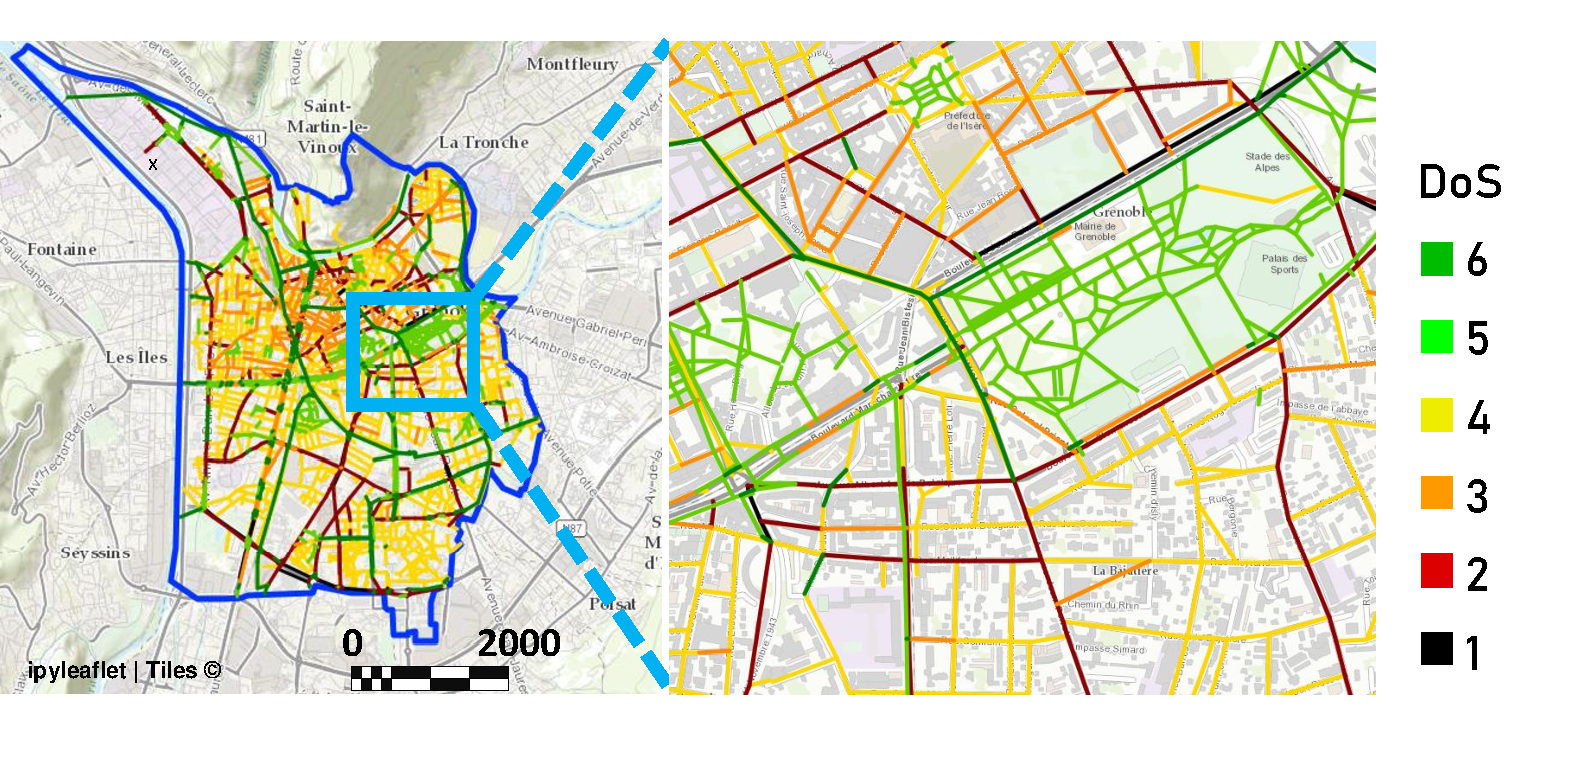
\includegraphics[width=1\columnwidth]{Images/Map_and_scale.pdf}
\caption{\footnotesize Cycling network of Grenoble, France. The degree of separation (DoS) score of the cycling infrastructure from motorized vehicles is indicated in ascending order from 1 to 6.}
\label{networks_classification}
\end{figure}


% % Measuring how different two transport networks are is closely related to optimal transport, where one seeks the most cost-efficient way to transform one distribution of mass into another. The resulting Wasserstein distance defines a metric on probability measures that has become a powerful tool in both pure and applied mathematics, with applications ranging from fluid dynamics to economics and imaging \cite{villani2008optimal,villani2021topics,santambrogio2015optimal}. In the context of networks, this viewpoint naturally extends to comparing distributions of weights, flows, or exposures supported on nodes and arcs.

% % More generally, network comparison can be seen as a relaxation of graph isomorphism: instead of asking whether two graphs are exactly the same, one asks how far apart they are under some structural metric. Simple baselines compare adjacency matrices via classical norms, but these are highly sensitive to node relabeling and local noise. Richer approaches compare global statistics (e.g., clustering coefficient, diameter, path-length distributions) or higher-order patterns such as graphlets and node roles, which have been shown to capture functional similarity across diverse biological and technological networks \cite{yaverouglu2014revealing,faisal2017grafene}. At a more analytic level, cut distance and graphon-based methods provide a limit-theoretic notion of distance between large graphs that supports accurate comparison of complex networks \cite{liu2018cut}, while spectral methods use eigenvalues of adjacency or Laplacian matrices as compact, label-invariant signatures of graph structure \cite{wilson2008study}.

% % A complementary line of work uses graph kernels to embed entire networks into Hilbert spaces, enabling kernel-based learning and comparison. Early results showed how to define positive definite kernels over labeled graphs despite the hardness of exact subgraph counting \cite{gartner2003graph}. Random-walk and marginalized graph kernels \cite{kashima2003marginalized,vishwanathan2010graph} further exploited walk-based feature spaces, with algorithmic advances that reduce their computational cost and make them practical for large-scale applications. In contrast to these general-purpose tools, our framework tailors the comparison to cycling safety by constructing exposure-weighted kernels and graphon-like representations that are constrained to preserve safety-relevant attributes across cities.


% % \textit{Network comparison}: Comparing two transport networks can be viewed as a relaxation of the classical graph isomorphism problem: instead of asking whether there exists a bijection that makes two adjacency structures identical, we ask how far apart their structures are under a suitable notion of distance \cite{chartrand2013first}. A current approach is to compare adjacency matrices directly using standard matrix norms (Euclidean, Manhattan, etc.), in line with classical ideas from data analysis and data mining \cite{hand2007principles}, but such measures are highly sensitive to node labelling and local perturbations.

% % To obtain more robust and interpretable comparisons, a variety of structural descriptors have been proposed. Global statistics such as clustering coefficient, diameter, or average path length provide coarse summaries of network organisation, while higher-order pattern counts (e.g., graphlets) and role-based features capture finer functional similarity across complex biological and technological networks \cite{yaverouglu2014revealing,faisal2017grafene}. Spectral methods instead use the eigenvalues of adjacency or Laplacian matrices as label-invariant signatures of graph structure, and the distance between spectra has been shown to track graph edit distance in many settings \cite{wilson2008study}. From a more analytical perspective, cut distance and graphon-based theory provide limit objects and metrics that allow one to compare large graphs in a size-agnostic way, with good empirical performance on a range of complex networks \cite{liu2018cut}.

% % A complementary line of work embeds graphs into reproducing kernel Hilbert spaces via graph kernels. Early contributions showed how to define positive definite kernels on labelled graphs despite the computational hardness of exact subgraph counting \cite{gartner2003graph}. Random-walk and marginalized graph kernels \cite{kashima2003marginalized,vishwanathan2010graph} exploit walk-based feature spaces while remaining computationally tractable, and have become standard tools for supervised and unsupervised learning on graphs.

% % All these approaches can be connected to the broader framework of optimal transport, which studies the most efficient way to redistribute mass from one configuration to another. The associated Wasserstein distances define geometrically meaningful metrics between probability measures and have found applications across analysis, PDEs, and applied fields such as imaging and economics \cite{villani2008optimal,villani2021topics,santambrogio2015optimal}. In our setting, this viewpoint underlies the way we compare exposure distributions and safety-relevant kernels on cycling networks, providing a principled notion of “distance” between cities that is sensitive to both weights and structure. Existing network comparison methods are typically applied to generic graphs or to operational performance metrics, but not to safety-specific attributes of cycling networks, and they rarely account jointly for multi-attribute exposure measures and differences in network size or resolution when drawing conclusions across cities.

% \textit{Network comparison:} Comparing two transport networks can be seen as a relaxation of graph isomorphism: instead of asking whether a bijection makes their adjacencies identical, we ask how far apart their structures are under a chosen distance \cite{chartrand2013first}. A simple approach is to compare adjacency matrices via standard norms (Euclidean, Manhattan, etc.), in line with classical data analysis and data mining ideas \cite{hand2007principles}, but such measures are highly sensitive to node labelling and local perturbations.

% More robust comparisons use structural descriptors. Global statistics such as clustering coefficient, diameter, and average path length provide coarse summaries, while higher-order pattern counts (graphlets) and role-based features capture finer functional similarity across complex networks \cite{yaverouglu2014revealing,faisal2017grafene}. Spectral methods use eigenvalues of adjacency or Laplacian matrices as label-invariant signatures, with spectral distances tracking graph edit distance in many cases \cite{wilson2008study}. From a more analytical viewpoint, cut distance and graphon theory offer limit objects and size-agnostic metrics with good empirical performance on diverse networks \cite{liu2018cut}. A complementary line embeds graphs into reproducing kernel Hilbert spaces via graph kernels. Early work defined positive definite kernels on labelled graphs despite the hardness of exact subgraph counting \cite{gartner2003graph}. Random-walk and marginalized kernels \cite{kashima2003marginalized,vishwanathan2010graph} exploit walk-based feature spaces while remaining computationally tractable, and are now standard tools for learning on graphs. All these approaches connect to optimal transport, which studies the most efficient way to redistribute mass. Wasserstein distances provide geometrically meaningful metrics between probability measures and have widespread applications in analysis and applied fields \cite{villani2008optimal,villani2021topics,santambrogio2015optimal}. In our setting, this viewpoint underlies how we compare exposure distributions and safety-relevant kernels on cycling networks, yielding a principled notion of “distance” between cities that is sensitive to both weights and structure. However, existing methods are rarely tailored to safety-specific attributes of cycling networks, nor do they jointly handle multi-attribute exposure measures and differences in network size or resolution when drawing cross-city conclusions. To the best of the authors' knowlarc, there is currently no framework that (i) clusters cycling networks under explicit safety constraints so as to preserve multi-attribute indicators such as flow, slope, and angular change, and (ii) compares the resulting networks in a size-independent and mathematically consistent way using exposure-based kernels.

% \textit{Statement of Contribution}: In this paper, we propose a mathematical framework for clustering large cycling networks in a way that explicitly preserves a composite safety indicator built from cyclist flow, traffic exposure, slope, and angular change. The method produces clustered (supernode and superarcs) representations that minimize the distortion of these safety attributes relative to the original network, while reducing all cities to comparable graphs of the same node cardinality. This, in turn, enables fair and scale-independent comparison of cycling-network safety across cities using exposure-based distance measures on the clustered networks.


\section{Introduction}
\label{introduction}

The health, environmental, and socio-economic benefits of cycling are well established, including improved cardiovascular health, reduced emissions and air pollution, lower transportation costs, and decreased traffic congestion \cite{garrard2012health, gotschi2016cycling}. Consequently, public authorities increasingly promote cycling as an alternative to motorized transport for short and medium trips. However, concerns about safety and comfort remain major barriers to cycling adoption \cite{fishman2012barriers}. Dedicated infrastructure that separates cyclists from motorized traffic significantly improves perceived safety and comfort and is associated with higher cycling uptake \cite{lawrence2018cyclist, broach2012cyclists}. Well-connected and high-quality cycling networks can substantially increase ridership \cite{pucher2011walking, pucher2017cycling}. Despite this, analyzing real-world cycling networks is challenging due to their size, spatial complexity, and the multiple interacting factors influencing route choice and perceived safety. Moreover, comparing the safety performance of cycling networks across cities in a fair and scale-independent manner remains an open problem, yet is crucial for transferring successful planning strategies between urban contexts.

We propose a mathematical framework to compare cycling-network safety across cities of different sizes and levels of detail. Large road graphs are compressed into cluster-based super-networks using a constrained, safety-aware $k$-means algorithm on a spectral embedding. This process preserves key attributes such as distance, slope, degree of separation, traffic exposure, flow, and angular change while limiting information loss. On the resulting clustered networks, we construct exposure-based kernels that enable structural similarity comparisons between cities. Experiments on real-world networks show that these representations retain safety-critical structure sufficiently to support consistent and interpretable cross-city comparisons.

\textit{Related work:} Our contribution builds on two research areas: transport-network clustering and network comparison.

\textit{Community detection:} Clustering and community detection are widely used to uncover structure in complex networks. Classical $k$-means \cite{hartigan1979algorithm} minimizes within-cluster variance, while graph-based methods identify densely connected node groups, including edge-betweenness \cite{girvan2002community}, modularity maximization \cite{clauset2004finding}, spectral methods \cite{newman2006finding}, and physics-inspired approaches \cite{wu2004finding}. In transportation research, clustering has been applied to traffic-flow analysis \cite{xia2007defining, gu2016unsupervised}, driving-style characterization \cite{gace2021driving}, and temporal pattern discovery \cite{weijermars2005analyzing}. For spatial networks, community detection supports control-region design and equity analysis \cite{haghbayan2021community}. In cycling studies, clustering has been used to design bike networks from demand patterns \cite{akbarzadeh2018designing} and to improve connectivity under budget constraints \cite{natera2020data}. However, existing methods are not explicitly designed to preserve cyclist-oriented safety attributes such as exposure, slope, traffic conditions, or angular change when compressing large networks for cross-city comparison.

\textit{Network comparison:} Comparing transport networks can be viewed as a relaxed form of graph isomorphism, where structural similarity is quantified by a distance metric \cite{chartrand2013first}. Direct comparisons of adjacency matrices are simple but sensitive to node labeling and local perturbations \cite{hand2007principles}. More robust approaches rely on structural descriptors, including global statistics, graphlets, role-based features \cite{yaverouglu2014revealing,faisal2017grafene}, and spectral signatures \cite{wilson2008study}. Graph kernels embed networks into reproducing kernel Hilbert spaces, enabling similarity comparisons via random walks or marginalized feature spaces \cite{gartner2003graph,kashima2003marginalized,vishwanathan2010graph}.  Optimal transport theory provides a complementary perspective, with Wasserstein distances offering meaningful metrics between distributions \cite{villani2008optimal,villani2021topics,santambrogio2015optimal}. In this work, this framework underpins the comparison of exposure distributions on clustered cycling networks. However, existing methods rarely account for safety-specific attributes or jointly address multi-attribute exposure and differences in network size when comparing cities.

\textit{Statement of Contribution:} We introduce a mathematical framework that clusters large cycling networks while explicitly preserving a composite safety indicator based on cyclist flow, traffic exposure, slope, and angular change. The resulting supernetwork representations minimize distortion of safety attributes and reduce all cities to graphs with identical node cardinality. This enables fair, scale-independent comparison of cycling-network safety across cities using exposure-based distance measures.



\section{Model Design}
\label{model_design}
In this section, we first present the bike lane classification and the graph representation. Next, we introduce the cyclist flow prediction model and the bi-level optimization problems: The first adopts a utilitarian perspective to minimize cyclists' traffic exposure, directing flows toward safer routes, and reducing high-traffic exposure to improve overall safety, while the second follows a sufficientarian perspective, aiming to reduce the number of cyclists falling below relative safety thresholds. Finally, we introduce the two algorithms designed to solve these NP-hard problems.



\begin{table}[t]
\centering
\vspace{0.2cm}
\begin{tabular}{|c|p{5cm}|c|}
\hline
\textbf{DoS}   & \textbf{Description} & \textbf{AADT (veh/day)} \\
\hline
$6$  & Dedicated bike lanes, fully separated from motor traffic. & 14 400 \\

$5$  & Bike lanes shared with pedestrians, separate from cars. & 16 000 \\ 

$4$  & Mixed-traffic roads (30 km/h) without designated bike lanes. & 960  \\

$3$  & Shared roads with cycling pictograms. & 3 120 \\

$2$  & Roads with painted bike lanes.  & 6 912 \\

$1$  & Unmarked shared car-bike lanes. & 8 448 \\
\hline
\end{tabular}
\caption{\footnotesize The degree of separation (DoS) categorizes bike lane infrastructure based on safety levels. The third column presents annual average daily traffic (AADT) on adjacent roads, sourced from the GTLVille platform in Grenoble \cite{gtlville2024}.}
\label{dos_table}
\end{table}
\subsection{Bike Lane  Safety classification}


The DoS classification, adapted from an OSM-based platform, categorizes cycling infrastructure based on separation from motor traffic. Table~\ref{dos_table} presents DoS categories, showing that higher-DoS lanes offer greater safety. These scores serve as weights in the network graph, modeling upgrades from lower to higher safety levels. The classification methodology is detailed in \cite{2024graphbased}. Fig.~\ref{networks_classification} visualizes these classifications in the Grenoble cycling network.



\subsection{Graph Representation}


Let the network be represented by a weighted directed graph (digraph) $\mathcal{G} = (\mathcal{V}, \mathcal{A}, \mathcal{W})$, where $\mathcal{V}$ is the set of nodes corresponding to intersections or road endpoints, $\mathcal{A}$ is the set of directed arcs representing roads, and $\mathcal{W}$ is the set of weights assigned to those arcs. For each arc $a = (u, v) \in \mathcal{A}$, with $u,v \in \mathcal{V}$, the weight $w_a \in \mathcal{W}$ represents the DoS associated with the link. The weights are assumed to be symmetric, meaning $w_{(u,v)} = w_{(v,u)}$. The geographical length of each arc $a$ is denoted by $d_a$.

\subsection{Cyclist Flows}
\label{section_flows}

Following \cite{mesbah2012bilevel}, we use an all-or-nothing (AON) traffic assignment model that assumes no congestion and assigns all demand $q_{(u,v)}$ from the EMD2020 survey \cite{SMMAG_EMD} to the shortest available path  between nodes $u,v \in \mathcal{V}$. This reflects typical cycling dynamics, where congestion effects are minimal. In this section, we formalize and adopt the cyclist distance proposed in \cite{cooper2017using}, which defines this distance using OpenStreetMap and Cardiff cycling flow data while incorporating infrastructure characteristics. Then, betweenness centrality is applied to estimate the flow distribution.

To account for cycling-specific factors, we use a modified distance metric that accounts for key factors influencing route choice. Let $\mathcal{V}$ denote the set of nodes in the network, and let $u, v \in \mathcal{V}$ be two nodes. The shortest path between $u$ and $v$ is represented as $p_{(u,v)} = (a_{1},\ldots, a_{k})$, where each arc $a~\in~p_{(u,v)}$ has a geographical length $d_{a}$, an angular change $\measuredangle_a$ (in degrees, either along $a$ or at junctions between consecutive arcs), a slope factor $s_{a}$ (which depends on the terrain slope $m_{a}$), and a traffic factor $f_{a}$ (that takes into account the flow of car traffic on roads adjacent to bike lanes). We define the cyclist distance $b_{(u,v)}$ between nodes $u$ and $v$ as

\begin{equation}
\label{cyclist_distance}
    b_{(u,v)} = \sum_{a \in p_{(u,v)}} \left( d_a \cdot s_a \cdot (f_a)^{\rho} \right) +  \sum_{a \in p_{(u,v)}} \measuredangle_a \cdot \kappa,
\end{equation}
where $\rho > 0$ and $\kappa > 0$ are calibration parameters controlling the influence of traffic conditions and angular changes, respectively.
The traffic factor $f_a$ is defined as
\begin{equation}
\label{f_a}
f_a = 
     \begin{cases}
\psi \cdot \exp{\left( x^{\text{AADT}}_{a} \right)} & \text{if } w_a < 5, \\
\psi \cdot 2.03 & \text{if } w_a = 5, \\
\psi & \text{if } w_a = 6.
\end{cases}
\end{equation}

Here, $x^{\text{AADT}}_{a}$ represents the annual average daily traffic (AADT) of the adjacent car lanes, expressed in thousands. The variable $w_a$ denotes the DoS of the bike lane $a$. According to \cite{cyclerap2024}, the impact of annual average daily traffic (AADT) is neutralized when $w_a \geq 5$, indicating full separation from car lanes. The factor 2.03 accounts for an observed increase in crash risk in shared spaces with pedestrians compared to separate, exclusive bicycle lanes \cite{mesimaki2021near}. The parameter $\psi$ is a scaling factor.  
Let $p_{(u,v)}$ be the shortest path between nodes $u$ and $v$ based on the cyclist distance in \eqref{cyclist_distance}. Since the origin-destination (OD) demand in our data is symmetric, each node acts as both an origin and a destination, ensuring balanced inflow and outflow. The flow conservation for paths is given by
\begin{equation}
\label{eq_shortest_path}
    \phi_{p_{(u,v)}} = q_{(u,v)},
\end{equation}
where $q_{(u,v)}$ represents the demand between nodes $u$ and $v$.  
Next, let $\mathbb{I}_{a \in p_{(u,v)}}$ be a binary variable indicating whether arc $a$ is part of the shortest path $p_{(u,v)}$. Then, the total cyclist flow on arc $a$, denoted as $\phi_a$, is
\begin{equation}
\begin{aligned}
\label{eq_flows}
  & \phi_{a}  = \sum_{u,v \in \mathcal{V}} q_{(u,v)} \cdot \mathbb{I}_{a \in p_{(u,v)}} \geq 0, \quad \forall a \in \mathcal{A}  \\
  & \Phi  = \sum_{a \in \mathcal{A}} \phi_{a}.
\end{aligned}
\end{equation}
This ensures that the total flow on each arc is the sum of all demands for trips passing through it, maintaining balance across the network due to the symmetry of the demand matrix. To assess cyclist exposure to traffic conditions, we introduce $\mathcal{E}$ as a general measure of exposure, defined for pahts in the network. This metric helps evaluate network improvements. For a shortest path $p_{(u,v)} = (a_1, \dots, a_k)$, cyclist exposure captures the combined effect of traffic-related risk and the distance of cyclist interaction with traffic, and is defined as
\begin{equation}
\label{exposure_def}
    \mathcal{E}_{p_{(u,v)}} = \sum_{a \in p_{(u,v)}} d_{a} \cdot f_{a} \cdot \phi_{a},
\end{equation}
where $\phi_{a}, d_{a}$ and $f_{a}$ are the normalized arc flow, length and traffic factor, respectively. For a single arc $a \in \mathcal{A}$, cyclist exposure simplifies to
\begin{equation}
\label{arc_exposure}
    \mathcal{E}_{a} = d_{a} \cdot f_{a} \cdot \phi_{a} \in  \left [ 0,1 \right ].
\end{equation}
Then, for the original network the total cyclist exposure is:
\begin{equation}
    \mathcal{E}^{\text{orig}} = \frac{1}{|\mathcal{A}|} \sum_{(v_{i},v_{j}) \in \mathcal{A}} \phi_{(v_{i},v_{j})} \cdot f(w_{(v_{i},v_{j})}) \cdot d_{(v_{i},v_{j})}.
\end{equation}

%%%%%%%%%%%%%%%%%%%%%%%%%%%%%%%%%%%%%%%%%%%%%%%%%%%%%%%%%%%%%%%%%%%%%%%%%%%%%%%%%%%%%%%%%%%%%%%%%%%%%%%%%%







%%%%%%%%%%%%%%%%%%%%%%%%%%%%%%%%%%%%%%%%%%%%%%%%%%%%%%%%%%%%%%%%%%%%%%%%%%%%%%%%%%%%%%%%%%%%%%%%%%%%%%%%%%


\subsection{Cluster Network Definition}
% Let the clusters be $\{C_{r_{1}}\}_{r=1}^k$, then the cluster network $\tilde{\mathcal{G}} = (\tilde{\mathcal{V}} = \{C_{r_{1}}\}, \tilde{\mathcal{A}}, \tilde{\mathcal{W}})$, and $\tilde{a} = (C_{r_{1}}, C_{r_{2}}) \in \tilde{\mathcal{A}}$ exists if there are nodes $v \in C_{r_{1}}$ and $v \in C_{r_{2}}$ such that $(u,v) \in \mathcal{A}$.

% The clustered network values can be categorized as either between clusters (Inter) or within clusters (Intra). To avoid confusion, we define $\mathcal{A}_{(C_{r_{1}},C_{r_{2}})}=\left \{(u,v)\in \mathcal{A} \mid u\in C_{r_{1}},v\in C_{r_{2}} \right \}$ as the set of arcs between clusters $C_{r_{1}}$ and $C_{r_{2}}$. Then we define the inter and intra-cluster weights as:
% \begin{align}
%  \tilde{w}^{\text{inter}}_{(C_{r_{1}},C_{r_{2}})} & =  \underset{a \in \mathcal{A}_{(C_{r_{1}},C_{r_{2}})}}{\text{arg min}} \, w_a, \\
%  \tilde{w}^{\text{intra}}_{C_{r_{1}}} &= \arg\min_{a \in C_{r}} w_a,
% \end{align}
%  representing the minimum DoS (highest risk) connection between clusters, while the intra-cluster weight represents the worst-case risk within cluster $C_{r_{1}}$.

Let $\mathcal{P} = \{C_1,\dots,C_k\}$ be a partition of the node set $\mathcal{V}$ into $k$ non-empty clusters.
We define the clustered network as $\tilde{\mathcal{G}} = (\tilde{\mathcal{V}}, \tilde{\mathcal{A}}, \tilde{\mathcal{W}})$,
where the supernode set is $\tilde{\mathcal{V}} = \mathcal{P} = \{C_1,\dots,C_k\}$.
For any pair of clusters $(C_r, C_{r'})$, we define the set of arcs between them as
\[
  \mathcal{A}(C_r, C_{r'})
  \;=\;
  \bigl\{ (u,v) \in \mathcal{A} \;\big|\; u \in C_r,\; v \in C_{r'} \bigr\}.
\]
We include a superarc $\tilde{a} = (C_r, C_{r'})$ in $\tilde{\mathcal{A}}$ if and only if
$\mathcal{A}(C_r, C_{r'}) \neq \varnothing$. The clustered arc weights are split into \emph{inter}- and \emph{intra}-cluster components.
For $r \neq r'$, the inter-cluster DoS weight between $C_r$ and $C_{r'}$ is defined as
\begin{equation}
  \tilde{w}^{\mathrm{inter}}_{(C_r, C_{r'})}
  \;=\;
  \min_{a \in \mathcal{A}(C_r, C_{r'})} w_a,
\end{equation}
i.e., the minimum DoS (highest-risk) connection between the two clusters. For intra-cluster connections, we write
\[
  \mathcal{A}(C_r)
  \;:=\;
  \mathcal{A}(C_r, C_r)
  \;=\;
  \bigl\{ (u,v) \in \mathcal{A} \;\big|\; u \in C_r,\; v \in C_r \bigr\},
\]
and define the intra-cluster DoS weight as
\begin{equation}
  \tilde{w}^{\mathrm{intra}}_{C_r}
  \;=\;
  \min_{a \in \mathcal{A}(C_r)} w_a,
\end{equation}
which represents the worst-case (highest-risk) connection within cluster $C_r$.


To enable flow and exposure analysis on the clustered network $\tilde{\mathcal{G}}$, we need to redefine the all-or-nothing traffic assignment approach for this aggregated representation. This requires establishing new rules for path selection and flow distribution across the clustered structure.


% \subsection{Clustered Cyclist Distance}
% Let $\tilde{p}_{(C_{r_{1}},C_{r_{2}})} = (\tilde{a}_1, \ldots, \tilde{a}_m)$ be the shortest path between clusters $C_{r_{1}}$ and $C_{r_{2}}$ in $\tilde{\mathcal{G}}$, where each inter-cluster arc $\tilde{a}~\in ~\tilde{p}_{(C_{r_{1}},C_{r_{2}})}$ connects clusters $C_{r_{1}}$ to $C_{r_{2}}$. The clustered cyclist distance combines:

% \begin{equation}
% \label{clustered_cyclist_distance}
% \tilde{b}_{(C_{r_{1}},C_{r_{2}})} = \underbrace{\sum_{\tilde{a} \in \tilde{p}_{(C_{r_{1}},C_{r_{2}})}} \tilde{b}^{\text{inter}}_{\tilde{a}}}_{\text{inter-cluster}} + \underbrace{\sum_{C_{r} \in \tilde{p}_{(C_{r_{1}},C_{r_{1}})}} \tilde{b}^{\text{intra}}_{C_{r}}}_{\text{intra-cluster}}
% \end{equation}
% where the inter-cluster component for each superarc $\tilde{a}~\in ~\tilde{p}_{(C_{r_{1}},C_{r_{1}})}$ is:
% \begin{equation}
% \tilde{b}^{\text{inter}}_{\tilde{a}} = \left( \tilde{d}^{\text{inter}}_{\tilde{a}} \cdot \tilde{s}^{\text{inter}}_{\tilde{a}} \cdot (\tilde{f}^{\text{inter}}_{\tilde{a}})^{\rho} \right) + \tilde{\measuredangle}^{\text{inter}}_{\tilde{a}} \cdot \kappa
% \end{equation}
% and the intra-cluster component for each supernode $C_{r}$ is:
% \begin{equation}
% \tilde{b}^{\text{intra}}_{C_{r}} = \left( \tilde{d}^{\text{intra}}_{C_{r}} \cdot \tilde{s}^{\text{intra}}_{C_{r}} \cdot (\tilde{f}^{\text{intra}}_{C_{r}})^{\rho} \right) + \tilde{\measuredangle}^{\text{intra}}_{C_{r}} \cdot \kappa
% \end{equation}
% where for inter-cluster connections ($C_{r_{1}} \neq C_{r_{2}}$):
% \begin{align}
% \tilde{d}^{\text{inter}}_{\tilde{a}} &= \frac{\sum_{a \in \mathcal{A}_{(C_{r_{1}},C_{r_{2}})}} d_a \cdot \phi_a}{\sum_{a \in \mathcal{A}_{(C_{r_{1}},C_{r_{2}})}} \phi_a}, \quad \text{(distance)}\\
% \tilde{s}^{\text{inter}}_{\tilde{a}} &= \frac{\sum_{a \in \mathcal{A}_{(C_{r_{1}},C_{r_{2}})}} s_a \cdot \phi_a}{\sum_{a \in \mathcal{A}_{(C_{r_{1}},C_{r_{2}})}} \phi_a}, \quad \text{(slope)}\\
% \tilde{f}^{\text{inter}}_{\tilde{a}} &= f_{a}(\tilde{w}^{\text{inter}}_{(C_{r_{1}},C_{r_{2}})}), \quad \text{(traffic factor)}\\
% \tilde{\measuredangle}^{\text{inter}}_{\tilde{a}} &= \frac{\sum_{a \in \mathcal{A}_{(C_{r_{1}},C_{r_{2}})}} \measuredangle_a \cdot \phi_a}{\sum_{a \in \mathcal{A}_{(C_{r_{1}},C_{r_{2}})}} \phi_a} \quad \text{(angular change)}.
% \end{align}
% For intra-cluster paths ($C_{r}$):
% \begin{equation}
% \begin{aligned}
% \tilde{d}^{\text{intra}}_{C_{r}} &= \frac{\sum_{a \in C_{r}} d_a \cdot \phi_a}{\sum_{a \in \mathcal{A}_{(C_{r_{1}},C_{r_{2}})}} \phi_a}, \quad \text{(distance)}\\
% \tilde{s}^{\text{intra}}_{C_{r}} &= \frac{\sum_{a \in C_{r}} s_a \cdot \phi_a}{\sum_{a \in C_{r}} \phi_a},\quad \text{(slope)} \\
% \tilde{f}^{\text{intra}}_{C_{r}} &= f_a( \tilde{w}^{\text{intra}}_{C_{r}}) \quad \text{(traffic factor)}\\
% \tilde{\measuredangle}^{\text{intra}}_{C_{r}} &= \frac{\sum_{a \in C_{r}} \measuredangle_a \cdot \phi_a}{\sum_{a \in C_{r}} \phi_a}, \quad \text{(angular change)}
% \end{aligned}
% \end{equation}
% \begin{remark}
% Our clustering methodology and cyclist distance formulation are designed to capture essential aspects of cycling behavior while maintaining computational efficiency. The key design choices are motivated by:
% \begin{itemize}
%     \item Using minimum DoS values for inter-cluster and intra-cluster connections follows a conservative approach that preserves route bottleneck safety, reflecting cyclists' tendency to avoid segments with high-risk infrastructure regardless of overall route quality.
%     \item The flow-weighted aggregation of distance, slope, and angular change parameters ensures that frequently used routes dominate cluster characteristics, mirroring actual cyclist experience patterns.
% \end{itemize}
% \end{remark}

\subsection{Clustered cyclist distance}

Let $\tilde{p}_{(C_r,C_{r'})} = (\tilde{a}_1,\dots,\tilde{a}_m)$ denote a shortest path
between clusters $C_r$ and $C_{r'}$ in the clustered network
$\tilde{\mathcal{G}}$,
where each superarc $\tilde{a}_\ell \in \tilde{p}_{(C_r,C_{r'})}$ connects two clusters.  
We write $\mathcal{C}(C_r,C_{r'}) \subseteq \tilde{\mathcal{V}}$ for the set of clusters
visited along this path (including $C_r$ and $C_{r'}$). The clustered cyclist distance between $C_r$ and $C_{r'}$ is defined as
\begin{equation}
\label{eq:clustered_cyclist_distance}
  \tilde{b}_{(C_r,C_{r'})}
  \;=\;
  \underbrace{\sum_{\tilde{a} \in \tilde{p}_{(C_r,C_{r'})}} 
    \tilde{b}^{\mathrm{inter}}_{\tilde{a}}}_{\text{inter-cluster}}
  \;+\;
  \underbrace{\sum_{C_q \in \mathcal{C}(C_r,C_{r'})}
    \tilde{b}^{\mathrm{intra}}_{C_q}}_{\text{intra-cluster}}.
\end{equation}
For each superarc $\tilde{a} = (C_r,C_{r'}) \in \tilde{\mathcal{A}}$ with $r \neq r'$,
the inter-cluster contribution is
\begin{equation}
  \tilde{b}^{\mathrm{inter}}_{\tilde{a}}
  \;=\;
  \bigl(
    \tilde{d}^{\mathrm{inter}}_{\tilde{a}}
    \cdot
    \tilde{s}^{\mathrm{inter}}_{\tilde{a}}
    \cdot
    (\tilde{f}^{\mathrm{inter}}_{\tilde{a}})^{\rho}
  \bigr)
  \;+\;
  \tilde{\measuredangle}^{\mathrm{inter}}_{\tilde{a}} \cdot \kappa,
\end{equation}
where the aggregated distance, slope, traffic factor and angular change are defined from the
underlying arcs between $C_r$ and $C_{r'}$:
\begin{align}
  \tilde{d}^{\mathrm{inter}}_{\tilde{a}}
  &=
  \frac{
    \sum_{a \in \mathcal{A}(C_r,C_{r'})} d_a \,\cdot \phi_a
  }{
    \sum_{a \in \mathcal{A}(C_r,C_{r'})} \phi_a
  },
  \quad\text{(distance)}\\[0.5em]
  \tilde{s}^{\mathrm{inter}}_{\tilde{a}}
  &=
  \frac{
    \sum_{a \in \mathcal{A}(C_r,C_{r'})} s_a \,\cdot \phi_a
  }{
    \sum_{a \in \mathcal{A}(C_r,C_{r'})} \phi_a
  },
  \quad\text{(slope)}\\[0.5em]
  \tilde{f}^{\mathrm{inter}}_{\tilde{a}}
  &=
  f_a\bigl(\tilde{w}^{\mathrm{inter}}_{(C_r,C_{r'})}\bigr),
  \quad\text{(traffic factor)}\\[0.5em]
  \tilde{\measuredangle}^{\mathrm{inter}}_{\tilde{a}}
  &=
  \frac{
    \sum_{a \in \mathcal{A}(C_r,C_{r'})} \measuredangle_a \,\cdot \phi_a
  }{
    \sum_{a \in \mathcal{A}(C_r,C_{r'})} \phi_a
  },
  \quad\text{(angular change)}.
\end{align}
For each cluster $C_r$, we define the set of intra-cluster arcs
\[
  \mathcal{A}(C_r)
  \;:=\;
  \mathcal{A}(C_r,C_r)
  \;=\;
  \bigl\{ (u,v) \in \mathcal{A} \,\big|\,
          u \in C_r,\; v \in C_r \bigr\}.
\]
The intra-cluster contribution of $C_r$ is
\begin{equation}
  \tilde{b}^{\mathrm{intra}}_{C_r}
  \;=\;
  \bigl(
    \tilde{d}^{\mathrm{intra}}_{C_r}
    \cdot
    \tilde{s}^{\mathrm{intra}}_{C_r}
    \cdot
    (\tilde{f}^{\mathrm{intra}}_{C_r})^{\rho}
  \bigr)
  \;+\;
  \tilde{\measuredangle}^{\mathrm{intra}}_{C_r} \cdot \kappa,
\end{equation}
with
\begin{align}
  \tilde{d}^{\mathrm{intra}}_{C_r}
  &=
  \frac{
    \sum_{a \in \mathcal{A}(C_r)} d_a \, \cdot \phi_a
  }{
    \sum_{a \in \mathcal{A}(C_r)} \phi_a
  },
  \quad\text{(distance)}\\[0.5em]
  \tilde{s}^{\mathrm{intra}}_{C_r}
  &=
  \frac{
    \sum_{a \in \mathcal{A}(C_r)} s_a \, \cdot \phi_a
  }{
    \sum_{a \in \mathcal{A}(C_r)} \phi_a
  },
  \quad\text{(slope)}\\[0.5em]
  \tilde{f}^{\mathrm{intra}}_{C_r}
  &=
  f_a\bigl(\tilde{w}^{\mathrm{intra}}_{C_r}\bigr),
  \quad\text{(traffic factor)}\\[0.5em]
  \tilde{\measuredangle}^{\mathrm{intra}}_{C_r}
  &=
  \frac{
    \sum_{a \in \mathcal{A}(C_r)} \measuredangle_a \, \cdot \phi_a
  }{
    \sum_{a \in \mathcal{A}(C_r)} \phi_a
  },
  \quad\text{(angular change)}.
\end{align}

\begin{remark}
Our clustering methodology and cyclist-distance formulation are designed to capture
essential aspects of cycling behaviour while remaining computationally tractable.
Key design choices include:
\begin{itemize}
  \item Using minimum DoS values for inter- and intra-cluster connections to follow a
  conservative, bottleneck-preserving perspective: a single high-risk segment can
  dominate perceived safety along a route.
  \item Aggregating distance, slope, traffic factor, and angular change via
  flow-weighted averages, so that frequently used segments dominate cluster-level
  characteristics and better reflect typical cyclist experience.
\end{itemize}
\end{remark}


% \textbf{Safety-First Principle:} 

% \textbf{Behaviorally-Grounded Metrics:} 

% \textbf{Empirical Risk Modeling:} The traffic factor $f_a$ incorporates:
% \begin{itemize}
%     \item Exponential AADT sensitivity for mixed traffic conditions
%     \item Documented 2.03× risk increase in pedestrian-shared spaces
%     \item Complete traffic isolation for fully separated lanes
% \end{itemize}

% \textbf{Adaptable Calibration:} Parameters $\rho$ and $\kappa$ provide flexibility to accommodate regional variations in cyclist preferences and local navigation complexities.

% \textbf{Multi-Scale Representation:} The separation into inter-cluster and intra-cluster components maintains both macroscopic routing decisions and microscopic local navigation, ensuring comprehensive safety assessment across spatial scales while enabling computationally efficient network analysis.

% \begin{equation}
% \begin{aligned}
% \mathcal{E}_{\text{clust}} = \frac{1}{|\tilde{\mathcal{A}}| + |\{C_p\}|} \Biggl( 
% &\underbrace{\sum_{(C_{r_{1}},C_{r_{2}}) \in \tilde{\mathcal{A}}} \tilde{\phi}^{\text{inter}}_{(C_{r_{1}},C_{r_{2}})} \cdot f^{\text{inter}}_{(C_{r_{1}},C_{r_{2}})} \cdot d^{\text{inter}}_{(C_{r_{1}},C_{r_{2}})}}_{\mathcal{E}^{\text{inter}}} \\
% &+ \underbrace{\sum_{C_{r} \in \left \{C_{p} \right\}} \tilde{\phi}^{\text{intra}}_{C_{r}} \cdot f^{\text{intra}}_{C_{r}} \cdot d^{\text{intra}}_{C_{r}}}_{\mathcal{E}^{\text{intra}}} 
% \Biggr)
% \end{aligned}
% \end{equation}


%%%%%%%%%%%%%%%%%%%%%%%%%%%%%
% \subsection{Clustered Demand and Flow Assignment}
% Given the original graph $\mathcal{G} = (\mathcal{V}, \mathcal{A}, \mathcal{W})$ and its clustered representation $\tilde{\mathcal{G}}=(\mathcal{C},\tilde{\mathcal{A}}, \tilde{\mathcal{W}})$, where $\mathcal{C}={C_1,\ldots,C_k}$ is the set of clusters, we define the clustered demand $\tilde{q}$ as follows: First, let $\chi: \mathcal{V} \rightarrow \mathcal{C}$ be the cluster assignment mapping that associates each node $v \in \mathcal{V}$ to its corresponding cluster $C_i \in \mathcal{C}$. The clustered demand between two clusters $C_{r_{1}}, C_{r_{2}} \in \mathcal{C}$ is computed by aggregating all original demands $q_{(u,v)}$ where $u \in C_{r_{1}}$ and $v \in C_{r_{2}}$:
% \begin{equation}
% \label{cluster_demand}
% \tilde{q}_{(C_{r_{1}},C_{r_{2}})} = \sum_{\substack{u \in C_{r_{1}} \ v \in C_{r_{2}}}} q_{(u,v)} \cdot \mathbb{I}_{{(u,v) \in \mathcal{A}}},
% \end{equation}
% where $\mathbb{I}_{{(u,v) \in \mathcal{A}}}$ is an indicator function that ensures only valid arcs in the original graph are considered. The all-or-nothing traffic assignment on the clustered graph $\tilde{\mathcal{G}}$ can be done by the all-or-nothing assignment as follows:
% Let $\tilde{p}_{(C_{r_{1}},C_{r_{2}})}$ be the shortest path between clusters $C_{r_{1}}$ and $C_{r_{2}}$ in $\tilde{\mathcal{G}}$. The inter-cluster flow of arc $\tilde{a} \in \mathcal{A}$ and the intra-cluster flow aggregates all flows within a cluster $C_{r} \in \mathcal{C}$ are defined as:
% \begin{align}
% \label{eq_cluster_flow_inter}
% \tilde{\phi}_{\tilde{a}}^{\text{inter}} & = \sum_{\substack{(C_{r_{1}}, C_{r_{2}})}} \tilde{q}_{(C_{r_{1}},C_{r_{2}})} \cdot \mathbb{I}_{\tilde{a} \in \tilde{p}_{(C_{r}, C_{r_{2}})}}, \\
% \tilde{\phi}_{C_{r}}^{\text{intra}} & = \sum_{\substack{(C_{r_{1}}, C_{r_{2}})}} \tilde{q}_{(C_{r_{1}},C_{r_{2}})} \cdot \mathbb{I}_{C_{r} \in \tilde{p}_{(C_{r}, C_{r_{2}})}},
% \end{align}
% where $\mathbb{I}_{\tilde{a} \in \tilde{p}_{(C_{r_{1}}, C_{r_{2}})}}$ is a binary indicator for whether the inter-cluster arc $\tilde{a}$ belongs to path $\tilde{p}_{(C_{r_{1}},C_{r_{2}})}$, similarly for $\mathbb{I}_{C_{r} \in \tilde{p}_{(C_{r}, C_{r_{2}})}}$.
% Then, for the cluster network $\tilde{\mathcal{G}}$ the total cyclist exposure is defined as the sum between the intra and inter cyclist exposure of the clusters:
% \begin{equation}
% \begin{aligned}
% \mathcal{E}^{\text{clust}} & = \frac{1}{|\tilde{\mathcal{A}}| + |\{C_p\}|} \Biggl( 
% \mathcal{E}^{\text{inter}} + \mathcal{E}^{\text{intra}} 
% \Biggr) \\
% \Phi^{\text{clust}} & = \Phi^{\text{intra}} + \Phi^{\text{inter}}
% \end{aligned}
% \end{equation}
% where 
% \begin{equation}
% \begin{aligned}
% \label{cluster_def}
% \mathcal{E}^{\text{inter}} & = \sum_{\tilde{a} \in \tilde{\mathcal{A}}} \tilde{\phi}^{\text{inter}}_{\tilde{a}} \cdot f^{\text{inter}}_{\tilde{a}} \cdot d^{\text{inter}}_{\tilde{a}} \\
% \mathcal{E}^{\text{inter}} & = \sum_{C_{r} \in \left \{C_{p} \right\}} \tilde{\phi}^{\text{intra}}_{C_{r}} \cdot f^{\text{intra}}_{C_{r}} \cdot d^{\text{intra}}_{C_{r}} \\
% \Phi^{\text{inter}} &= \sum_{\tilde{a} \in \tilde{\mathcal{A}}} 
% \tilde{\phi}^{\text{inter}}_{\tilde{a}} \\
% \Phi^{\text{intra}} &= \sum_{C_{r} \in \left \{C_{p} \right\}} \tilde{\phi}^{\text{intra}}_{C_{r}}
% \end{aligned}
% \end{equation}
%%%%%%%%%%%%%%%%%%%%%%%%%%%%%


\subsection{Clustered demand, flow assignment, and exposure}

Given the original graph $\mathcal{G}$ and its clustered representation $\tilde{\mathcal{G}}$. The clustered demand between two clusters $C_r, C_{r'} \in \mathcal{C}$ is obtained by aggregating the
original OD demands $q_{(u,v)}$ with origins in $C_r$ and destinations in $C_{r'}$:
\begin{equation}
\label{cluster_demand}
  \tilde{q}_{(C_r,C_{r'})}
  \;:=\;
  \sum_{\substack{u \in C_r \\ v \in C_{r'}}}
  q_{(u,v)} \, \cdot \mathbb{I}_{(u,v) \in \mathcal{A}},
\end{equation}
where $\mathbb{I}_{(u,v) \in \mathcal{A}}$ is an indicator function that ensures only valid arcs in the original graph are considered.  
For the all-or-nothing assignment on the clustered graph, let $\tilde{p}_{(C_r,C_{r'})}$ denote a shortest path between $C_r$ and $C_{r'}$ in $\tilde{\mathcal{G}}$,
computed with respect the clustered cyclist distance.
We define the inter-cluster flow on a superarc $\tilde{a} \in \tilde{\mathcal{A}}$ as
\begin{equation}
\label{eq_cluster_flow_inter}
  \tilde{\phi}^{\mathrm{inter}}_{\tilde{a}}
  \;:=\;
  \sum_{(r,r')}\,
    \tilde{q}_{(C_r,C_{r'})}\; \cdot 
    \mathbb{I}_{\tilde{a} \in \tilde{p}_{(C_r,C_{r'})}},
\end{equation}
where $\mathbb{I}_{\tilde{a} \in \tilde{p}_{(C_r,C_{r'})}}$ indicates whether the superarc $\tilde{a}$ lies on the
shortest path between $C_r$ and $C_{r'}$. Similarly, we define the intra-cluster flow associated with a cluster $C_r \in \mathcal{C}$ as the total clustered
demand whose shortest path traverses $C_r$:
\begin{equation}
  \tilde{\phi}^{\mathrm{intra}}_{C_r}
  \;:=\;
  \sum_{(r_1,r_2)}\,
    \tilde{q}_{(C_{r_1},C_{r_2})}\; \cdot
    \mathbb{I}_{C_r \in \tilde{p}_{(C_{r_1},C_{r_2})}},
\end{equation}
where $\mathbb{I}_{C_r \in \tilde{p}_{(C_{r_1},C_{r_2})}}$ is $1$ if the path between $C_{r_1}$ and $C_{r_2}$ passes
through cluster $C_r$, and $0$ otherwise. With all these, finally, on the clustered network $\tilde{\mathcal{G}}$, we define the total cyclist exposure as the average of the inter- and
intra-cluster contributions:
\begin{equation}
\begin{aligned}
  \mathcal{E}^{\mathrm{clust}}
  &:= \frac{1}{\,|\tilde{\mathcal{A}}| + |\mathcal{C}|\,}
      \Bigl(
        \mathcal{E}^{\mathrm{inter}} + \mathcal{E}^{\mathrm{intra}}
      \Bigr), \\[0.4em]
  \Phi^{\mathrm{clust}}
  &:= \Phi^{\mathrm{inter}} + \Phi^{\mathrm{intra}}.
\end{aligned}
\end{equation}
Here, the inter- and intra-cluster exposure terms are
\begin{equation}
\label{cluster_def}
\begin{aligned}
  \mathcal{E}^{\mathrm{inter}}
  &:= \sum_{\tilde{a} \in \tilde{\mathcal{A}}}
        \tilde{\phi}^{\mathrm{inter}}_{\tilde{a}}\, \cdot
        f^{\mathrm{inter}}_{\tilde{a}}\, \cdot
        d^{\mathrm{inter}}_{\tilde{a}}, \\[0.4em]
  \mathcal{E}^{\mathrm{intra}}
  &:= \sum_{r=1}^k
        \tilde{\phi}^{\mathrm{intra}}_{C_r}\, \cdot
        f^{\mathrm{intra}}_{C_r}\, \cdot
        d^{\mathrm{intra}}_{C_r},
\end{aligned}
\end{equation}
and the corresponding total flows are
\begin{equation}
\begin{aligned}
  \Phi^{\mathrm{inter}}
  &:= \sum_{\tilde{a} \in \tilde{\mathcal{A}}}
        \tilde{\phi}^{\mathrm{inter}}_{\tilde{a}}, \\[0.4em]
  \Phi^{\mathrm{intra}}
  &:= \sum_{r=1}^k
        \tilde{\phi}^{\mathrm{intra}}_{C_r}.
\end{aligned}
\end{equation}
The quantities $d^{\mathrm{inter}}_{\tilde{a}}, f^{\mathrm{inter}}_{\tilde{a}}$ and
$d^{\mathrm{intra}}_{C_r}, f^{\mathrm{intra}}_{C_r}$ are the clustered distance and traffic-factor
terms defined in the previous subsection for inter- and intra-cluster connections, respectively.
%%%%%%%%%%%%%%%%%%%%%%%%%%%%%%



% \begin{figure*}
% \label{clustering_benchmark}
%   \centering
%   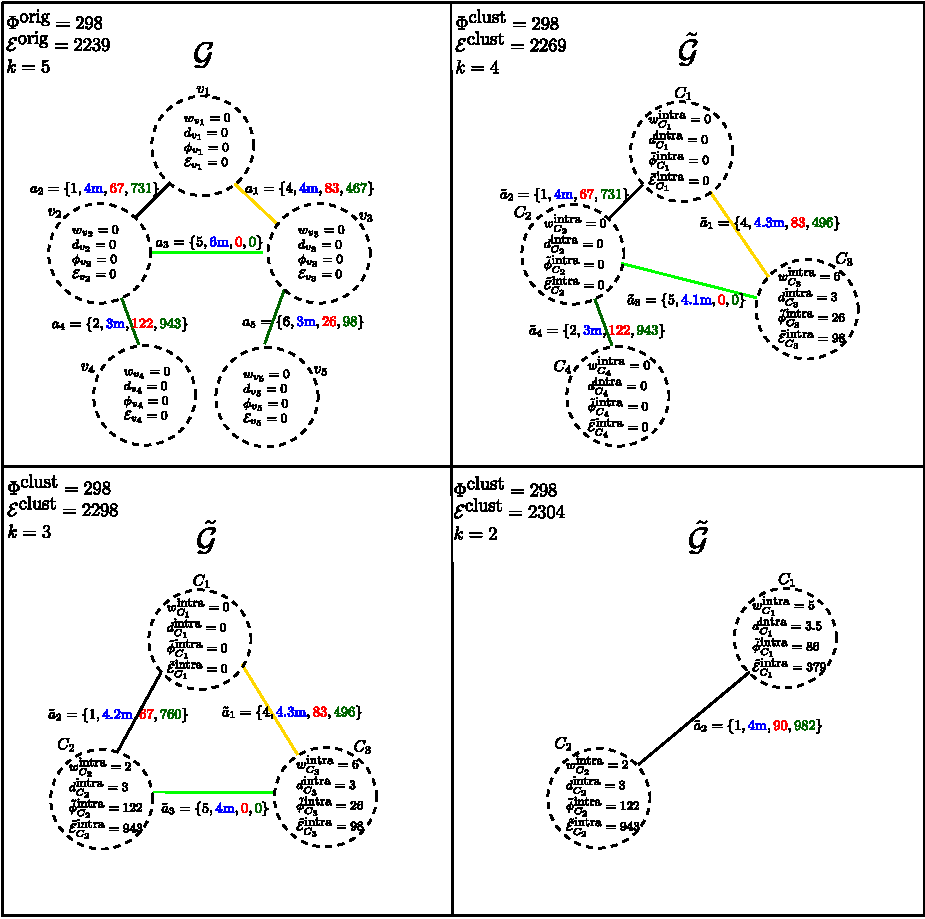
\includegraphics[width=0.7\textwidth]{Images/03_09_2025.pdf}
%   \caption{Algorithm 1 for toy example where $a~=~\left \{w_{a} , \textcolor{blue}{d_{a} (\mbox{m})}, \textcolor{red}{\phi_{a}}, \textcolor{DarkGreen}{\mathcal{E}_{a}} \right \}$, $\tilde{a}^{\mbox{inter}}~=~\left \{w^{\mbox{inter}}_{\tilde{a}} , \textcolor{blue}{d^{\mbox{inter}}_{\tilde{a}} (\mbox{m})}, \textcolor{red}{\phi^{\mbox{inter}}_{\tilde{a}}}, \textcolor{DarkGreen}{\mathcal{E}^{\mbox{inter}}_{\tilde{a}}} \right \}$, and $C^{\mbox{intra}}~=~\left \{d^{\mbox{intra}}_{C} , \textcolor{blue}{d^{\mbox{intra}}_{C} (\mbox{m})}, \textcolor{red}{\phi^{\mbox{inter}}_{C}}, \textcolor{DarkGreen}{\mathcal{E}^{\mbox{intra}}_{C}} \right \}$}
% \end{figure*}




\begin{figure*}[h!]
\vspace{0.2cm}
  \centering
  \captionsetup[subfigure]{font={footnotesize}, labelfont={footnotesize, bf}, textfont={footnotesize, rm}}

  \subfloat[Original]{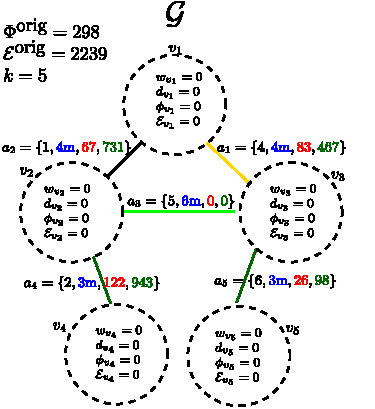
\includegraphics[width=0.24\linewidth]{Images/G.pdf}\label{fig::ae_orig}}
  \hspace{0.001\linewidth}
  % \hspace{0.001\linewidth} % Adjust horizontal space as needed
  \subfloat[Cluster $k=4$]
  {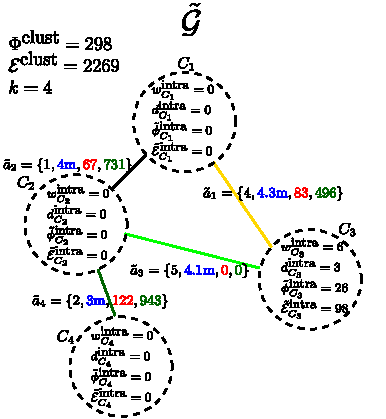
\includegraphics[width=0.24\linewidth]{Images/G_4.pdf}\label{fig::ae_4}} 
  \hspace{0.001\linewidth} % Adjust horizontal space as needed
  \subfloat[Cluster $k=3$]{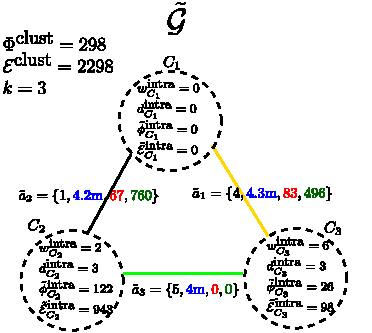
\includegraphics[width=0.24\linewidth]{Images/G_3.pdf}\label{fig::ae_3}}
  \hspace{0.001\linewidth} % Adjust vertical space as needed
  \subfloat[Cluster $k=2$]{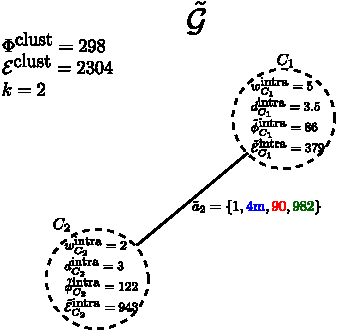
\includegraphics[width=0.24\linewidth]{Images/G_2.pdf}\label{fig::ae_2}}
  \caption{\footnotesize Algorithm 1 for toy example where $a~=~\left \{w_{a} , \textcolor{blue}{d_{a} (\mbox{m})}, \textcolor{red}{\phi_{a}}, \textcolor{DarkGreen}{\mathcal{E}_{a}} \right \}$, $\tilde{a}^{\mbox{inter}}~=~\left \{w^{\mbox{inter}}_{\tilde{a}} , \textcolor{blue}{d^{\mbox{inter}}_{\tilde{a}} (\mbox{m})}, \textcolor{red}{\phi^{\mbox{inter}}_{\tilde{a}}}, \textcolor{DarkGreen}{\mathcal{E}^{\mbox{inter}}_{\tilde{a}}} \right \}$, and $C^{\mbox{intra}}~=~\left \{d^{\mbox{intra}}_{C} , \textcolor{blue}{d^{\mbox{intra}}_{C} (\mbox{m})}, \textcolor{red}{\phi^{\mbox{inter}}_{C}}, \textcolor{DarkGreen}{\mathcal{E}^{\mbox{intra}}_{C}} \right \}$}
  \label{fig:ae_clustering}
\end{figure*}


% \section{Clustering Algorithm}

% To enable fair comparison between two networks of different sizes (in terms of cyclist exposure $\mathcal{E}$ or cyclist flow $\Phi$), we cluster the larger network to match the number of nodes in the smaller one. This produces a reduced representation $\tilde{\mathcal{G}}$ in which each supernode $C_p$ may represent an entire neighborhood in the original network. The resulting clustered graph preserves the structural and cycling-specific properties (DoS, distance, slope, traffic factor) required for analysis, enabling the use of metrics such as the Wasserstein distance for cross-network comparison.

% We construct the spectral embedding from the weighted adjacency matrix
% \begin{equation}
% \label{eq:adjacency_matrix}
% A_{ij} = 
% \begin{cases}
% w_{ij} \cdot \exp\!\left(-\frac{d_{ij}}{\gamma}\right) \cdot \left(\frac{\phi_{ij}}{\max \phi}\right)^\alpha & \text{if } (i,j) \in \mathcal{A}, \\
% 0 & \text{otherwise},
% \end{cases}
% \end{equation}
% where $\gamma > 0$ controls spatial locality and $\alpha \geq 0$ regulates the effect of high-flow arcs. The normalized Laplacian $\mathcal{L}~=~I~-~D^{-1/2}AD^{-1/2}$, with $D_{ii} = \sum_j A_{ij}$, provides the input for the spectral clustering.

% The constrained clustering procedure is summarized in Algorithm~\ref{alg:constrained-clustering-math}. Original total flow $\Phi^{\text{orig}}$ and total exposure $\mathcal{E}^{\text{orig}}$ are computed from \eqref{eq_flows} and \eqref{exposure_def} respectively; their clustered counterparts $\Phi^{\text{clust}}$ and $\mathcal{E}^{\text{clust}}$ follow from the definitions in eq.~ \eqref{cluster_def} and the clustered network formulation.

% The algorithm uses the following notation: $k$ represents the number of clusters, $\epsilon_{\max}$ denotes the maximum allowed DoS variation within a cluster, $\delta_{\max}$ specifies the maximum spatial diameter of a cluster, $\Delta\mathcal{E}_{\max}$ defines the maximum permissible exposure difference (typically set to 10\%), $\Delta\Phi_{\max}$ establishes the maximum flow difference threshold, and $\alpha_{\text{relax}}$ serves as the relaxation factor for gradually adjusting constraints when necessary.

% This algorithm implements several important features to ensure effective clustering. First, it progressively relaxes the exposure and flow bounds ($\tau_{\mathcal{E}}$ and $\tau_{\Phi}$) while maintaining strict adherence to the fundamental DoS and distance constraints. Second, it incorporates Lagrangian terms ($\lambda_1$ and $\lambda_2$) during the k-means clustering process to penalize any violations of the specified constraints. Finally, as a fallback mechanism, the algorithm reverts to standard unconstrained k-means clustering if no feasible solution can be found that satisfies all the imposed conditions, ensuring that some clustering solution is always produced.

\section{Clustering Algorithm}

To enable fair comparison between two cycling networks of different sizes, we cluster the larger network so that its number of supernodes matches the number of nodes in the smaller one. The construction of $\tilde{\mathcal{G}}$ is designed to preserve safety-relevant attributes (DoS, distance, slope, traffic factor, flow, and exposure), so that the clustered network remains comparable in safety terms to the original. We first build a safety-aware weighted adjacency matrix
\begin{equation}
\label{eq:adjacency_matrix}
A_{ij} =
\begin{cases}
w_{ij}\,\cdot \exp\!\Bigl(-\dfrac{d_{ij}}{\gamma}\Bigr) \cdot
\left(\dfrac{\phi_{ij}}{\max \phi}\right)^{\alpha} & \text{if } (i,j)\in\mathcal{A},\\[0.6em]
0 & \text{otherwise},
\end{cases}
\end{equation}
where $w_{ij}$ is DoS, $d_{ij}$ is the spatial distance, $\phi_{ij}$ is the cyclist flow on arc $(i,j)$, $\gamma~>~0$ controls spatial locality and $\alpha~\geq~0$ regulates the influence of high-flow arcs. The normalized Laplacian
\[
  \mathcal{L} = I - D^{-1/2} A D^{-1/2},
  \qquad D_{ii} = \sum_j A_{ij},
\]
provides a spectral embedding on which we run $k$-means. Now we proceed to build a constrained $k$-means, let $\Phi^{\mathrm{orig}}$ and $\mathcal{E}^{\mathrm{orig}}$ denote the total flow and exposure on $\mathcal{G}$ (cf.~\eqref{eq_flows} and \eqref{exposure_def}), and let $\Phi^{\mathrm{clust}}$ and $\mathcal{E}^{\mathrm{clust}}$ be their clustered counterparts defined in \eqref{cluster_def} and the previous subsection. The clustering is performed by a constrained $k$-means procedure (Algorithm~\ref{alg:constrained-clustering-math} with pseudo-code in Appendix A) with the following parameters:

\textit{$i)$} $\epsilon_{\max}$: maximum allowed DoS variation within any cluster $C_r$ (e.g., $\epsilon_{\max}=2$ allows clusters of at most two levels of DoS separation),

\textit{$ii)$}  $\delta_{\max}$: maximum spatial diameter of a cluster, making sure that all arcs in the group are relatively close to each other,

\textit{$iii)$} $\tau_{\mathcal{E}}^{(0)} :=\frac{\bigl|\mathcal{E}^{\mathrm{clust}} - \mathcal{E}^{\mathrm{orig}}\bigr|}{\mathcal{E}^{\mathrm{orig}}}$: initial tolerance on the relative exposure difference,
        
\textit{$iv)$} $\tau_{\Phi}^{(0)}:= \frac{\bigl|\Phi^{\mathrm{clust}} - \Phi^{\mathrm{orig}}\bigr|}{\Phi^{\mathrm{orig}}}$: initial tolerance on the relative flow difference, 
        
\textit{$v)$}  $\alpha_{\mathrm{relax}}$: relaxation factor for gradually enlarging $\tau_{\mathcal{E}}$ and $\tau_{\Phi}$ if needed.


At each iteration, $k$-means is run in the spectral space with a modified objective that adds Lagrangian penalties $\lambda_1,\lambda_2$ for violating the exposure and flow constraints, while hard constraints enforce DoS homogeneity and bounded spatial diameter inside each cluster. If no feasible solution is found under the current tolerances, the algorithm increases $\tau_{\mathcal{E}}$ and $\tau_{\Phi}$ by a factor $\alpha_{\mathrm{relax}}>1$ and retries. As a safety valve, if the constrained problem remains infeasible, the method falls back to standard unconstrained $k$-means in the same spectral embedding, ensuring that a clustering $\mathcal{C}=\{C_1,\dots,C_k\}$ is always produced. In this way, the clustered network $\tilde{\mathcal{G}}$ approximates the original exposure and flow while strictly controlling intra-cluster safety heterogeneity and spatial extent, which is crucial for fair, safety-aware comparison across cities.



\subsection{Mathematical Guarantees}
We start by demonstrating that the Laplacian defined, is indeed a Laplacian:
\begin{theorem}
The matrix $\mathcal{L} = I - D^{-1/2}AD^{-1/2}$ is a valid symmetric normalized graph Laplacian.
\end{theorem}

\begin{proof}
The proof is shown in Appendix A.
\end{proof}

\subsubsection*{Parameter Determination}
The parameters $\gamma > 0$ and $\alpha \geq 0$ in Eq.~\eqref{eq:adjacency_matrix} control the influence of spatial distance and flow magnitude, respectively, on the adjacency weights. They must be chosen to ensure the resulting graph structure reflects meaningful connectivity for clustering. The proof of the Laplacian's properties holds for any $\gamma > 0$ and $\alpha \geq 0$. Therefore, the Laplacian $\mathcal{L}$ maintains its fundamental properties for any admissible choice of $\gamma$ and $\alpha$. These parameters should be calibrated based on the specific network and desired clustering outcome, for instance, by ensuring the eigenvalues of $\mathcal{L}$ exhibit a clear gap to suggest a natural number of clusters $k$.
% \begin{theorem}[Flow Preservation in Network Clustering]
% \label{thm:flow_preservation}
% Given a di-graph $\mathcal{G} = (\mathcal{V}, \mathcal{A}, \mathcal{W})$ with demand matrix $q_{(u,v)}$ and its clustered representation $\tilde{\mathcal{G}} = (\tilde{\mathcal{V}}, \tilde{\mathcal{A}}, \tilde{\mathcal{W}})$ constructed via Algorithm~\ref{alg:constrained-clustering-math}, the total network flow is preserved:
% \[
% \Phi^{\text{orig}} \triangleq \sum_{a \in \mathcal{A}} \phi_a = \sum_{\tilde{a} \in \tilde{\mathcal{A}}} \tilde{\phi}_{\tilde{a}} = \Phi^{\text{clust}}.
% \]
% \end{theorem}
% \begin{proof}
% Observe that the clustered demand $\tilde{q}_{(C_{r_{1}},C_{r_{2}})}$ in \eqref{cluster_demand} aggregates all original demands between nodes in clusters $C_{r_{1}}$ and $C_{r_{2}}$ as $\tilde{q}_{(C_{r_{1}},C_{r_{2}})} = \sum_{u \in C_{r_{1}}, v \in C_{r_{2}}} q_{(u,v)}$, ensuring total demand preservation $\sum_{u,v \in \mathcal{V}} q_{(u,v)} = \sum_{C_{r_{1}},C_{r_{2}} \in \tilde{\mathcal{V}}} \tilde{q}_{(C_{r_{1}},C_{r_{2}})}$. 

% In the original graph $\mathcal{G}$, the all-or-nothing assignment \eqref{eq_flows} yields arc flows $\phi_a~=~\sum_{u,v} q_{(u,v)} \cdot \mathbb{I}_{a \in p_{(u,v)}}$, while in the clustered graph $\tilde{\mathcal{G}}$, \eqref{eq_cluster_flow_inter} gives superarc flows $\tilde{\phi}_{\tilde{a}}~=~\sum_{C_{r_{1}},C_{r_{2}}} \tilde{q}_{(C_{r_{1}},C_{r_{2}})} \cdot \mathbb{I}_{\tilde{a} \in \tilde{p}_{(C_{r_{1}},C_{r_{2}})}}$.  The total flow in $\mathcal{G}$ decomposes as:
% \begin{align}
% \Phi^{\text{orig}} & = \sum_{a \in \mathcal{A}} \phi_a = \sum_{u,v} q_{(u,v)} \underbrace{\sum_{a \in \mathcal{A}} \mathbb{I}_{a \in p_{(u,v)}}}_{=1} \\
% & = \sum_{u,v} q_{(u,v)},
% \end{align}
% since each path $p_{(u,v)}$ covers exactly one set of arcs. Similarly, for $\tilde{\mathcal{G}}$:
% \begin{align}
% \Phi^{\text{clust}} &= \sum_{\tilde{a} \in \tilde{\mathcal{A}}} \tilde{\phi}_{\tilde{a}} = \sum_{C_{r_{1}},C_{r_{2}}} \tilde{q}_{(C_{r_{1}},C_{r_{2}})} \underbrace{\sum_{\tilde{a} \in \tilde{\mathcal{A}}}}_{=1} \mathbb{I}_{\tilde{a} \in \tilde{p}_{(C_{r_{1}},C_{r_{2}})}} \\
% & = \sum_{C_{r_{1}},C_{r_{2}}} \tilde{q}_{(C_{r_{1}},C_{r_{2}})},
% \end{align}
% where the indicator sums equal 1 because each clustered path $\tilde{p}_{(C_{r_{1}},C_{r_{2}})}$ traverses exactly one sequence of superarcs. By demand conservation, we conclude $\Phi^{\text{orig}} \equiv \Phi^{\text{clust}}$.
% \end{proof}

\begin{theorem}[Flow Preservation in Network Clustering]
\label{thm:flow_preservation}
Given a di-graph $\mathcal{G} = (\mathcal{V}, \mathcal{A}, \mathcal{W})$ with demand matrix $q_{(u,v)}$ and its clustered representation $\tilde{\mathcal{G}} = (\tilde{\mathcal{V}}, \tilde{\mathcal{A}}, \tilde{\mathcal{W}})$ constructed via Algorithm~\ref{alg:constrained-clustering-math}, the total network flow is preserved:
\[
\Phi^{\text{orig}} \triangleq \sum_{a \in \mathcal{A}} \phi_a
= \sum_{\tilde{a} \in \tilde{\mathcal{A}}} \tilde{\phi}_{\tilde{a}}
= \Phi^{\text{clust}}.
\]
\end{theorem}

\begin{proof}
The proof is shown in Appendix A.
\end{proof}




% \begin{proof}
% Observer that the clustered demand $\tilde{q}_{(C_{r_{1}},C_{r_{2}})}$ in \eqref{cluster_demand} aggregates all original demands between nodes in clusters $C_{r_{1}}$ and $C_{r_{2}}$:
%     \[
%     \tilde{q}_{(C_{r_{1}},C_{r_{2}})} = \sum_{\substack{u \in C_{r_{1}} \\ v \in C_{r_{2}}}} q_{(u,v)},
%     \]
%     ensuring total demand preservation:
%     \[
%     \sum_{u,v \in \mathcal{V}} q_{(u,v)} = \sum_{C_{r_{1}},C_{r_{2}} \in \tilde{\mathcal{V}}} \tilde{q}_{(C_{r_{1}},C_{r_{2}})}.
%     \]
%     In $\mathcal{G}$, the AON assignment \eqref{eq_flows} gives $\phi_a = \sum_{u,v} q_{(u,v)} \cdot \mathbb{I}_{a \in p_{(u,v)}}$. Meanwhile in $\tilde{\mathcal{G}}$, \eqref{eq_cluster_flow_inter} gives $\tilde{\phi}_{\tilde{a}} = \sum_{C_{r_{1}},C_{r_{2}}} \tilde{q}_{(C_{r_{1}},C_{r_{2}})} \cdot \mathbb{I}_{\tilde{a} \in \tilde{p}_{(C_{r_{1}},C_{r_{2}})}} $, and then,
%     summing all arc flows in $\mathcal{G}$ we obtain a flow assignment equivalence:
%     \begin{align}
%         \Phi^{\text{orig}} & = \sum_{a \in \mathcal{A}} \sum_{u,v} q_{(u,v)} \cdot \mathbb{I}_{a \in p_{(u,v)}} \nonumber \\
%         & = \sum_{u,v} q_{(u,v)} \underbrace{\sum_{a \in \mathcal{A}} \mathbb{I}_{a \in p_{(u,v)}}}_{=1} = \sum_{u,v} q_{(u,v)},
%     \end{align}
    
%     and in $\tilde{\mathcal{G}}$:
%     \begin{align}
%         \Phi^{\text{clust}} & = \sum_{\tilde{a} \in \tilde{\mathcal{A}}} \sum_{C_{r_{1}},C_{r_{2}}} \tilde{q}_{(C_{r_{1}},C_{r_{2}})} \mathbb{I}_{\tilde{a}} \in \tilde{p}_{(C_{r_{1}},C_{r_{2}})} \nonumber \\
%         & = \sum_{C_{r_{1}},C_{r_{2}}} \tilde{q}_{(C_{r_{1}},C_{r_{2}})} \underbrace{\sum_{\tilde{a}} \mathbb{I}_{\tilde{a}} \in \tilde{p}_{(C_{r_{1}},C_{r_{2}})}}_{=1} = \sum_{C_{r_{1}},C_{r_{2}}} \tilde{q}_{(C_{r_{1}},C_{r_{2}})}.
%     \end{align}
%     By demand conservation, $\Phi^{\text{orig}} = \Phi^{\text{clust}}$.
% \end{proof}

% \begin{proof}
% The proof establishes flow preservation through three sequential arguments:

% First, demand conservation follows directly from the clustering definition. The clustered demand $\tilde{q}_{(C_{r_{1}},C_{r_{2}})}$ in \eqref{cluster_demand} sums all origin-destination pairs between clusters:
% \begin{align}
% \tilde{q}_{(C_{r_{1}},C_{r_{2}})} &= \sum_{\substack{u \in C_{r_{1}} \\ v \in C_{r_{2}}}} q_{(u,v)}, \quad\text{thus} \\
% \sum_{u,v \in \mathcal{V}} q_{(u,v)} &= \sum_{C_{r_{1}},C_{r_{2}} \in \tilde{\mathcal{V}}} \tilde{q}_{(C_{r_{1}},C_{r_{2}})}.
% \end{align}

% Second, the all-or-nothing assignment preserves flows through path aggregation. In $\mathcal{G}$, each arc's flow accumulates from all paths using it:
% \begin{align}
% \phi_a &= \sum_{u,v} q_{(u,v)} \cdot \mathbb{I}_{a \in p_{(u,v)}}, \\
% \Rightarrow \Phi^{\text{orig}} &= \sum_{a \in \mathcal{A}} \phi_a = \sum_{u,v} q_{(u,v)} \underbrace{\sum_{a \in \mathcal{A}} \mathbb{I}_{a \in p_{(u,v)}}}_{=1 \text{ (per-path flow)}}.
% \end{align}
% Analogously for $\tilde{\mathcal{G}}$:
% \begin{align}
% \tilde{\phi}_{\tilde{a}} &= \sum_{C_{r_{1}},C_{r_{2}}} \tilde{q}_{(C_{r_{1}},C_{r_{2}})} \cdot \mathbb{I}_{\tilde{a} \in \tilde{p}_{(C_{r_{1}},C_{r_{2}})}}, \\
% \Rightarrow \Phi^{\text{clust}} &= \sum_{\tilde{a} \in \tilde{\mathcal{A}}} \tilde{\phi}_{\tilde{a}} = \sum_{C_{r_{1}},C_{r_{2}}} \tilde{q}_{(C_{r_{1}},C_{r_{2}})} \underbrace{\sum_{\tilde{a}} \mathbb{I}_{\tilde{a} \in \tilde{p}_{(C_{r_{1}},C_{r_{2}})}}}_{=1}.
% \end{align}

% The critical insight is that both networks distribute flows completely: every unit of demand is assigned to some path (original or clustered), and each path's flow contributes exactly once to the total. Combining this with demand conservation yields:
% \begin{equation}
% \Phi^{\text{orig}} = \sum_{u,v} q_{(u,v)} \equiv \sum_{C_{r_{1}},C_{r_{2}}} \tilde{q}_{(C_{r_{1}},C_{r_{2}})} = \Phi^{\text{clust}}. \qedhere
% \end{equation}
% \end{proof}

%%%%%%%%%%%%%%%%%%%%%%%%%%%%%%%%%%%%%Corollary and remarks
% \begin{remark}
% The preservation holds for any clustering that:
% \begin{enumerate}
%     \item Maintains the original demand sum via \eqref{cluster_demand},
%     \item Uses all-or-nothing assignment on shortest paths.
% \end{enumerate}
% \end{remark}


% \begin{corollary}[Exposure Approximation Bound]
% \label{cor:exposure_bound}
% Under the conditions of Theorem~\ref{thm:flow_preservation}, the cyclist exposure $\mathcal{E}$ satisfies:
% \[
% \left| \mathcal{E}^{\text{orig}} - \mathcal{E}^{\text{clust}} \right| \leq \Delta\mathcal{E}_{\max},
% \]
% where $\Delta\mathcal{E}_{\max}$ is the tolerance in Algorithm~\ref{alg:constrained-clustering-math}.
% \end{corollary}

% \begin{proof}
% The deviation arises from three approximations in $\tilde{\mathcal{G}}$: \\
% \textit{$i):$} arc lengths $d_a$ are averaged to $\tilde{d}^{\text{inter/intra}}$, \\
% \textit{$ii):$} Traffic factors $f_a$ become $$\tilde{f}^{\text{inter/intra}} = f(\min_{a \in \mathcal{A}_{(C_{r_{1}},C_{r_{2}})}} w_a),$$ \\
% \textit{$iii):$} Aggregation redistributes $\phi_a$ to superarcs $\tilde{\phi}_{\tilde{a}}$. \\
% Algorithm~\ref{alg:constrained-clustering-math} controls the error by iteratively relaxing $\tau_{\mathcal{E}}$ until the exposure difference meets $\Delta\mathcal{E}_{\max}$.
% \end{proof}

% \begin{remark}
% The bound is tight when high-flow arcs cluster with geometrically/safety-similar neighbors. For skewed flow distributions (e.g., commute corridors), prioritize clustering these arcs first.
% \end{remark}


%%%%%%%%%%%%%%%%%%%%%%%%%%%%%%%%%%%%%%%%%%%%%%%%%%%%%%%%%%
\section{Network Comparison}
\label{sec:gw_comparison}

% To compare the networks $\mathcal{G}$ (for instance Paris) and $\mathcal{H}$ (for instance Grenoble) where $|\mathcal{V}^\mathcal{G}| > |\mathcal{V}^\mathcal{H}|$, we proceed in three stages. \\
% \textit{$i):$ Network Clustering.} The Paris network $\mathcal{G}$ is clustered into $\tilde{\mathcal{G}}$ using Algorithm~\ref{alg:constrained-clustering-math} such that $|\tilde{\mathcal{V}}| = |\mathcal{V}^\mathcal{H}|$. This ensures equal cardinality while preserving flow properties (Theorem~\ref{thm:flow_preservation}).\\
% \textit{$ii):$ Exposure Distribution Construction.} For each node $v_i$ in any network $\mathcal{K} \in \{\mathcal{H}, \tilde{\mathcal{G}}\}$, define its exposure density as:
% \begin{align}
% \label{node_exposure_def}
% \mu_\mathcal{E}^\mathcal{K}(v_i) &= \frac{1}{Z^\mathcal{K}} \left( \left [  \sum_{a \in \mathcal{A}^\mathcal{K}(v_i)} \mathcal{E}_a \right ] + \mathcal{E}^{\text{intra}}_{v_{i}} \right), \\ 
% Z^\mathcal{K} & = \sum_{v_i \in \mathcal{V}^\mathcal{K}} \left( \sum_{a \in \mathcal{A}^\mathcal{K}(v_i)} \mathcal{E}_a + \epsilon \right)
% \end{align}
% where $\mathcal{A}^\mathcal{K}(v_i)$ denotes arcs incident to $v_i$, and $\epsilon = 10^{-6}$ prevents zero-mass nodes. Note that the previous equation for supernodes is $C_p \in \tilde{\mathcal{V}}$, the exposure aggregates intra-cluster and boundary arcs:
% \[
% \mu_\mathcal{E}^{\tilde{\mathcal{G}}}(C_r) = \frac{1}{Z^{\tilde{\mathcal{G}}}} \left( \sum_{a \in C_r} \mathcal{E}_a + \sum_{\tilde{a} \in \tilde{\mathcal{A}}(C_r)} \tilde{\mathcal{E}}_{\tilde{a}} + \epsilon \right).
% \]
% \textit{$iii):$ Distance Computation.} The Gromov-Wasserstein distance $GW_2(\tilde{\mathcal{G}}, \mathcal{H})$ is computed through four steps: First, construct intra-network distance matrices $$(D_X^{\tilde{\mathcal{G}}})_{r_{1}r_{2}} = |\mu_\mathcal{E}^{\tilde{\mathcal{G}}}(C_{r_{1}}) - \mu_\mathcal{E}^{\tilde{\mathcal{G}}}(C_{r_{2}})| + \gamma \| \mathbf{c}_{r_{1}} - \mathbf{c}_{r_{2}} \|_2$$ 
% for $\tilde{\mathcal{G}}$ and analogously $(D_X^\mathcal{H})_{ij}$ for $\mathcal{H}$. Second, define the cross-network distance $$(D_{X\tilde{X}})_{pi} = |\mu_\mathcal{E}^{\tilde{\mathcal{G}}}(C_p) - \mu_\mathcal{E}^\mathcal{H}(v_i)| + \gamma \| \mathbf{c}_p - \mathbf{x}_i \|_2$$
% Third, solve the optimization problem:
% \begin{equation}
% \label{gw_distance}
% GW_2 = \inf_{\pi \in \Pi} \sqrt{ \sum_{\substack{p,q \in \tilde{\mathcal{V}} \\ i,j \in \mathcal{V}^\mathcal{H}}}} |(D_X^{\tilde{\mathcal{G}}})_{pq} - (D_X^\mathcal{H})_{ij}|^2 \pi_{pi} \pi_{qj} 
% \end{equation}
% where the coupling $\pi$ satisfies $\sum_{i} \pi_{pi} = \mu_\mathcal{E}^{\tilde{\mathcal{G}}}(C_p)$ and $\sum_{p} \pi_{pi} = \mu_\mathcal{E}^\mathcal{H}(v_i)$. Fourth, interpret $\pi_{pi}$ as the optimal transport plan between Paris supernodes and Grenoble nodes.


%%%%%%%%%%%%%%%%%%%%%%%%%%%%%%%%%%%%%%%%%%%%%
% \subsection*{Safety-based distances between networks}

% We compare the original cycling network $\mathcal{G}$ and the clustered network $\tilde{\mathcal{H}}$ via three complementary metrics.  
% Let $\mathcal{G} = (\mathcal{V}^G,\mathcal{A}^G,\mathcal{W}^G)$ and $\tilde{\mathcal{H}} = (\mathcal{C},\tilde{\mathcal{A}},\tilde{\mathcal{W}})$ with $|\mathcal{V}^G| = |\mathcal{C}| =: n$.  
% For each node $v_i \in \mathcal{V}^G$ and cluster $C_r \in \mathcal{C}$ we denote by $m_i^G$ and $m_r^{\tilde{H}}$ the associated \emph{node-exposure mass} (sum of incident edge exposure plus intra-cluster exposure), and by $x_i^G,\,x_r^{\tilde{H}} \in \mathbb{R}^2$ their geographic positions (longitude–latitude or centroids).

% \paragraph{Wasserstein distance on exposure distributions.}
% We define exposure measures
% \[
% M^G \;=\; \sum_{i=1}^n m_i^G, 
% \qquad
% M^{\tilde{H}} \;=\; \sum_{r=1}^n m_r^{\tilde{H}},
% \]
% \[
% \mu^G \;=\; \frac{1}{M^G} \sum_{i=1}^n m_i^G\,\delta_{x_i^G},
% \qquad
% \mu^{\tilde{H}} \;=\; \frac{1}{M^{\tilde{H}}} \sum_{r=1}^n m_r^{\tilde{H}}\,\delta_{x_r^{\tilde{H}}},
% \]
% where $\delta_x$ is the Dirac mass at $x$.  
% For a ground metric $d:\mathbb{R}^2\times\mathbb{R}^2 \to \mathbb{R}_+$ (we use Euclidean distance) and $p \ge 1$, the $p$-Wasserstein distance is
% \[
% W_p^p\!\left(\mu^G,\mu^{\tilde{H}}\right)
% \;=\;
% \min_{\pi \in \Pi(\mu^G,\mu^{\tilde{H}})}
% \sum_{i=1}^n \sum_{r=1}^n d\!\left(x_i^G,x_r^{\tilde{H}}\right)^p \,\pi_{ir},
% \]
% where $\Pi(\mu^G,\mu^{\tilde{H}})$ is the set of couplings with marginals $\mu^G$ and $\mu^{\tilde{H}}$.  
% We report $W_p(\mu^G,\mu^{\tilde{H}})$ (typically $p=1$ or $p=2$) as a global distance between exposure distributions.

% \paragraph{SSIM on rasterized exposure fields.}
% We rasterize node-exposure onto a common grid using a fixed bounding box for both cities, obtaining images
% \[
% I_G,\, I_{\tilde{H}} \in [0,1]^{N_x \times N_y},
% \]
% where each pixel stores the (normalized) exposure in that spatial cell.  
% Let $\mu_G, \mu_{\tilde{H}}$ be the mean intensities, $\sigma_G^2, \sigma_{\tilde{H}}^2$ the variances, and $\sigma_{G\tilde{H}}$ the covariance of $(I_G, I_{\tilde{H}})$.  
% The (global) structural similarity index is
% \[
% \operatorname{SSIM}(I_G, I_{\tilde{H}}) \;=\;
% \frac{(2\mu_G \mu_{\tilde{H}} + c_1)(2\sigma_{G\tilde{H}} + c_2)}
%      {(\mu_G^2 + \mu_{\tilde{H}}^2 + c_1)(\sigma_G^2 + \sigma_{\tilde{H}}^2 + c_2)},
% \]
% with standard stability constants $c_1, c_2 > 0$.  
% Higher SSIM values indicate more similar spatial organization of cyclist exposure.

% \paragraph{Kernel / graphon distance on exposure kernels.}
% We construct exposure kernels $K^G, K^{\tilde{H}} \in \mathbb{R}_+^{n \times n}$ in a common node ordering (e.g., sorted by geographic coordinates), with entries
% \[
% K^G_{ij} \;=\; \sum_{\substack{a=(v_i,v_j)\in\mathcal{A}^G}} \mathrm{exposure}_a,
% \qquad
% K^{\tilde{H}}_{rr'} \;=\; \sum_{\substack{\tilde{a}=(C_r,C_{r'})\in\tilde{\mathcal{A}}}} \mathrm{exposure}_{\tilde{a}},
% \]
% including both inter-cluster exposure and intra-cluster contributions on the diagonal.  
% We normalize each kernel to sum~$1$,
% \[
% \hat{K}^G \;=\; \frac{K^G}{\sum_{i,j} K^G_{ij}},
% \qquad
% \hat{K}^{\tilde{H}} \;=\; \frac{K^{\tilde{H}}}{\sum_{r,r'} K^{\tilde{H}}_{rr'}},
% \]
% and interpret them as discrete graphons on $\{1,\dots,n\}^2$.  
% Our kernel-based graph distance is the mean absolute difference
% \[
% d_{\text{ker}}(\mathcal{G},\tilde{\mathcal{H}})
% \;=\;
% \frac{1}{n^2}
% \sum_{i=1}^n \sum_{j=1}^n
% \bigl|\hat{K}^G_{ij} - \hat{K}^{\tilde{H}}_{ij}\bigr|,
% \]
% which measures how much the pairwise exposure structure changes when passing from $\mathcal{G}$ to $\tilde{\mathcal{H}}$ under a common node ordering.
%%%%%%%%%%%%%%%%%%%%%%%%%%%%%%%%%%%%%%%%%%%%%
%%%%%%%%%%%%%%%%%%%%%%%%%%%%%%%%%%%%%%%%%%%%%%%%%

% The purpose of this work is to enable a fair safety comparison between a cycling network $\mathcal{G}$ and a smaller one $\mathcal{H} = (\mathcal{V}(\mathcal{H}),\mathcal{A}(\mathcal{H}),\mathcal{W}(\mathcal{H}))$ by clustering $\mathcal{G}$ into $\tilde{\mathcal{G}}= (\mathcal{C},\tilde{\mathcal{A}},\tilde{\mathcal{W}})$ such that $|\mathcal{V}(\mathcal{H})| = |\mathcal{C}| =: n$. For each node $v_i \in \mathcal{V}(\mathcal{H})$ and cluster $C_r \in \mathcal{C}$ we define a \emph{node-exposure weight} by aggregating incident exposure.

% Let $\mathcal{E}_{ij}$ denote the exposure on arc $(v_i,v_j)\in\mathcal{A}(\mathcal{H})$. We set
% \begin{equation}
%   \omega_i^H
%   \;=\;
%   \sum_{\substack{(v_i,v_j)\in \mathcal{A}(\mathcal{H})}} \mathcal{E}_{ij}
%   \;+\;
%   \sum_{\substack{(v_j,v_i)\in \mathcal{A}(\mathcal{H})}} \mathcal{E}_{ji},
%   \qquad v_i \in \mathcal{V}(\mathcal{H}),
% \end{equation}
% i.e., the total exposure of all arcs incident to $v_i$. For the clustered graph $\tilde{\mathcal{G}}$, let $\tilde{\mathcal{E}}_{rr'}$ be the exposure on the inter-cluster arc $(C_r,C_{r'})\in \tilde{\mathcal{A}}$ and $\tilde{\mathcal{E}}^{\text{intra}}_{C_r}$ the intra-cluster exposure of $C_r$. We define
% \begin{equation}
%   \omega_r^{\tilde{G}}
%   \;=\;
%   \sum_{\substack{(C_r,C_{r'})\in \tilde{\mathcal{A}}}} \tilde{\mathcal{E}}_{rr'}
%   \;+\;
%   \sum_{\substack{(C_{r'},C_r)\in \tilde{\mathcal{A}}}} \tilde{\mathcal{E}}_{r'r}
%   \;+\;
%   \tilde{\mathcal{E}}^{\text{intra}}_{C_r},
%   \qquad C_r \in \mathcal{C},
% \end{equation}
% so that intra- and inter-cluster exposure both contribute to the supernode weight.  
% Let $x_i^H, x_r^{\tilde{G}} \in \mathbb{R}^2$ be the geographic coordinates (longitude–latitude or centroids) of $v_i$ and $C_r$, respectively.

% \paragraph{Wasserstein distance on exposure distributions.}
% We first normalize node-exposure weights into probability measures. Define total exposure
% \[
% \Omega^H \;=\; \sum_{i=1}^n \omega_i^H,
% \qquad
% \Omega^{\tilde{G}} \;=\; \sum_{r=1}^n \omega_r^{\tilde{G}},
% \]
% and the corresponding discrete measures
% \[
% \mu^H \;=\; \frac{1}{\Omega^H} \sum_{i=1}^n \omega_i^H\,\delta_{x_i^H},
% \qquad
% \mu^{\tilde{G}} \;=\; \frac{1}{\Omega^{\tilde{G}}} \sum_{r=1}^n \omega_r^{\tilde{G}}\,\delta_{x_r^{\tilde{G}}},
% \]
% where $\delta_x$ is the Dirac mass at $x$.  

% For a ground metric $d:\mathbb{R}^2\times\mathbb{R}^2 \to \mathbb{R}_+$ (we use Euclidean distance) and $p \ge 1$, the $p$-Wasserstein distance between $\mu^H$ and $\mu^{\tilde{G}}$ is
% \[
% W_p^p\!\left(\mu^H,\mu^{\tilde{G}}\right)
% \;=\;
% \min_{\pi \in \Pi(\mu^H,\mu^{\tilde{G}})}
% \sum_{i=1}^n \sum_{r=1}^n d\!\left(x_i^H,x_r^{\tilde{G}}\right)^p \,\pi_{ir},
% \]
% where $\Pi(\mu^H,\mu^{\tilde{G}})$ is the set of couplings with marginals $\mu^H$ and $\mu^{\tilde{G}}$.  
% We report $W_p(\mu^H,\mu^{\tilde{G}})$ (typically $p=1$ or $p=2$) as a global distance between exposure distributions.

% \paragraph{SSIM on rasterized exposure fields.}
% We rasterize node-exposure onto a common grid using a fixed bounding box for both cities, obtaining images
% \[
% I_H,\, I_{\tilde{G}} \in [0,1]^{N_x \times N_y},
% \]
% where each pixel stores the (normalized) exposure in that spatial cell.  
% Let $\mu_H, \mu_{\tilde{G}}$ be the mean intensities, $\sigma_H^2, \sigma_{\tilde{G}}^2$ the variances, and $\sigma_{H\tilde{G}}$ the covariance of $(I_H, I_{\tilde{G}})$.  
% The (global) structural similarity index is
% \[
% \operatorname{SSIM}(I_H, I_{\tilde{G}}) \;=\;
% \frac{(2\mu_H \mu_{\tilde{G}} + c_1)(2\sigma_{H\tilde{G}} + c_2)}
%      {(\mu_H^2 + \mu_{\tilde{G}}^2 + c_1)(\sigma_H^2 + \sigma_{\tilde{G}}^2 + c_2)},
% \]
% with standard stability constants $c_1, c_2 > 0$.  
% Higher SSIM values indicate more similar spatial organization of cyclist exposure.

% \paragraph{Kernel / graphon distance on exposure kernels.}
% We construct exposure kernels $K^H, K^{\tilde{G}} \in \mathbb{R}_+^{n \times n}$ in a common node ordering (e.g., sorted by geographic coordinates), with entries
% \[
% K^H_{ij} \;=\; \sum_{\substack{a=(v_i,v_j)\in\mathcal{A}(\mathcal{H})}} \mathrm{exposure}_a,
% \qquad
% K^{\tilde{G}}_{rr'} \;=\; \sum_{\substack{\tilde{a}=(C_r,C_{r'})\in\tilde{\mathcal{A}}}} \mathrm{exposure}_{\tilde{a}},
% \]
% including both inter-cluster exposure and intra-cluster contributions on the diagonal.  
% We normalize each kernel to sum~$1$,
% \[
% \hat{K}^H \;=\; \frac{K^H}{\sum_{i,j} K^H_{ij}},
% \qquad
% \hat{K}^{\tilde{G}} \;=\; \frac{K^{\tilde{G}}}{\sum_{r,r'} K^{\tilde{G}}_{rr'}},
% \]
% and interpret them as discrete graphons on $\{1,\dots,n\}^2$.  
% Our kernel-based graph distance is the mean absolute difference
% \[
% d_{\text{ker}}(\mathcal{H},\tilde{\mathcal{G}})
% \;=\;
% \frac{1}{n^2}
% \sum_{i=1}^n \sum_{j=1}^n
% \bigl|\hat{K}^H_{ij} - \hat{K}^{\tilde{G}}_{ij}\bigr|,
% \]
% which measures how much the pairwise exposure structure changes when passing from $\mathcal{H}$ to $\tilde{\mathcal{G}}$ under a common node ordering.

%%%%%%%%%%%%%%%%%%%%%%%%%%%%%%%%%%%%%%%%%%%%%%%%%

% The purpose of this work is to enable a fair safety comparison between a cycling network $\mathcal{G}$ and a smaller one $\mathcal{H} = (\mathcal{V}(\mathcal{H}),\mathcal{A}(\mathcal{H}),\mathcal{W}(\mathcal{H}))$ by clustering $\mathcal{G}$ into $\tilde{\mathcal{G}}= (\mathcal{C},\tilde{\mathcal{A}},\tilde{\mathcal{W}})$ such that $|\mathcal{V}(\mathcal{H})| = |\mathcal{C}| =: n$. For each node $v_i \in \mathcal{V}(\mathcal{H})$ and cluster $C_r \in \mathcal{C}$ we define a \emph{node-exposure weight} by aggregating incident exposure.

% Let $\mathcal{E}_{ij}$ denote the exposure on arc $(v_i,v_j)\in\mathcal{A}(\mathcal{H})$. We set
% \begin{equation}
%   \omega_i^H
%   \;=\;
%   \sum_{\substack{(v_i,v_j)\in \mathcal{A}(\mathcal{H})}} \mathcal{E}_{ij}
%   \;+\;
%   \sum_{\substack{(v_j,v_i)\in \mathcal{A}(\mathcal{H})}} \mathcal{E}_{ji},
%   \qquad v_i \in \mathcal{V}(\mathcal{H}),
% \end{equation}
% i.e., the total exposure of all arcs incident to $v_i$. For the clustered graph $\tilde{\mathcal{G}}$, let $\tilde{\mathcal{E}}_{rr'}$ be the exposure on the inter-cluster arc $(C_r,C_{r'})\in \tilde{\mathcal{A}}$ and $\tilde{\mathcal{E}}^{\text{intra}}_{C_r}$ the intra-cluster exposure of $C_r$. We define
% \begin{equation}
%   \omega_r^{\tilde{G}}
%   \;=\;
%   \sum_{\substack{(C_r,C_{r'})\in \tilde{\mathcal{A}}}} \tilde{\mathcal{E}}_{rr'}
%   \;+\;
%   \sum_{\substack{(C_{r'},C_r)\in \tilde{\mathcal{A}}}} \tilde{\mathcal{E}}_{r'r}
%   \;+\;
%   \tilde{\mathcal{E}}^{\text{intra}}_{C_r},
%   \qquad C_r \in \mathcal{C},
% \end{equation}
% so that intra- and inter-cluster exposure both contribute to the supernode weight.  
% Let $x_i^H, x_r^{\tilde{G}} \in \mathbb{R}^2$ be the geographic coordinates (longitude–latitude or centroids) of $v_i$ and $C_r$, respectively.

% \paragraph{Wasserstein distance on exposure distributions.}
% We first normalize node-exposure weights into probability measures. Define total exposure
% \[
% \Omega^H \;=\; \sum_{i=1}^n \omega_i^H,
% \qquad
% \Omega^{\tilde{G}} \;=\; \sum_{r=1}^n \omega_r^{\tilde{G}},
% \]
% and the corresponding discrete measures
% \[
% \mu_H \;=\; \frac{1}{\Omega^H} \sum_{i=1}^n \omega_i^H\,\delta_{x_i^H},
% \qquad
% \mu_{\tilde{G}} \;=\; \frac{1}{\Omega^{\tilde{G}}} \sum_{r=1}^n \omega_r^{\tilde{G}}\,\delta_{x_r^{\tilde{G}}},
% \]
% where $\delta_x$ is the Dirac mass at $x$.  

% For a ground metric $d:\mathbb{R}^2\times\mathbb{R}^2 \to \mathbb{R}_+$ (we use Euclidean distance) and $p \ge 1$, the $p$-Wasserstein distance between $\mu_H$ and $\mu_{\tilde{G}}$ is
% \[
% W_p^p\!\left(\mu_H,\mu_{\tilde{G}}\right)
% \;=\;
% \min_{\pi \in \Pi(\mu_H,\mu_{\tilde{G}})}
% \sum_{i=1}^n \sum_{r=1}^n d\!\left(x_i^H,x_r^{\tilde{G}}\right)^p \,\pi_{ir},
% \]
% where $\Pi(\mu_H,\mu_{\tilde{G}})$ is the set of couplings with marginals $\mu_H$ and $\mu_{\tilde{G}}$.  
% We report $W_p(\mu_H,\mu_{\tilde{G}})$ (typically $p=1$ or $p=2$) as a global distance between exposure distributions.

% \paragraph{SSIM on rasterized exposure fields.}
% We rasterize node-exposure onto a common grid using a fixed bounding box for both cities, obtaining images
% \[
% I_H,\, I_{\tilde{G}} \in [0,1]^{N_x \times N_y},
% \]
% where each pixel stores the (normalized) exposure in that spatial cell.  
% Let $\mu(I_H), \mu(I_{\tilde{G}})$ be the mean intensities, $\sigma^2(I_H), \sigma^2(I_{\tilde{G}})$ the variances, and $\sigma(I_H,I_{\tilde{G}})$ the covariance of $(I_H, I_{\tilde{G}})$.  
% The (global) structural similarity index is
% \[
% \operatorname{SSIM}(I_H, I_{\tilde{G}}) \;=\;
% \frac{\bigl(2\,\mu(I_H)\,\mu(I_{\tilde{G}}) + c_1\bigr)\bigl(2\,\sigma(I_H,I_{\tilde{G}}) + c_2\bigr)}
%      {\bigl(\mu(I_H)^2 + \mu(I_{\tilde{G}})^2 + c_1\bigr)\bigl(\sigma^2(I_H) + \sigma^2(I_{\tilde{G}}) + c_2\bigr)},
% \]
% with standard stability constants $c_1, c_2 > 0$.  
% Higher SSIM values indicate more similar spatial organization of cyclist exposure.

% \paragraph{Kernel / graphon distance on exposure kernels.}
% We construct exposure kernels $K^H, K^{\tilde{G}} \in \mathbb{R}_+^{n \times n}$ in a common node ordering (e.g., sorted by geographic coordinates), with entries
% \[
% K^H_{ij} \;=\; \sum_{\substack{a=(v_i,v_j)\in\mathcal{A}(\mathcal{H})}} \mathrm{exposure}_a,
% \qquad
% K^{\tilde{G}}_{rr'} \;=\; \sum_{\substack{\tilde{a}=(C_r,C_{r'})\in\tilde{\mathcal{A}}}} \mathrm{exposure}_{\tilde{a}},
% \]
% including both inter-cluster exposure and intra-cluster contributions on the diagonal.  
% We normalize each kernel to sum~$1$,
% \[
% \hat{K}^H \;=\; \frac{K^H}{\sum_{i,j} K^H_{ij}},
% \qquad
% \hat{K}^{\tilde{G}} \;=\; \frac{K^{\tilde{G}}}{\sum_{r,r'} K^{\tilde{G}}_{rr'}},
% \]
% and interpret them as discrete graphons on $\{1,\dots,n\}^2$.  
% Our kernel-based graph distance is the mean absolute difference
% \[
% d_{\text{ker}}(\mathcal{H},\tilde{\mathcal{G}})
% \;=\;
% \frac{1}{n^2}
% \sum_{i=1}^n \sum_{j=1}^n
% \bigl|\hat{K}^H_{ij} - \hat{K}^{\tilde{G}}_{ij}\bigr|,
% \]
% which measures how much the pairwise exposure structure changes when passing from $\mathcal{H}$ to $\tilde{\mathcal{G}}$ under a common node ordering.

%%%%%%%%%%%%%%%%%%%%%%%%%%%%%%%%%%%%%%%%%%%%%%%%%
%%%%%%%%%%%%%%%%%%%%%%%%%%%%%%%%%%%%%%%%%%%%%%%%%
%%%%%%%%%%%%%%%%%%%%%%%%%%%%%%%%%%%%%%%%%%%%%%%%%
% The purpose of this work is to be able to a fair safety comparison between a cycling network $\mathcal{G}$ with an smaller one $\mathcal{H} = (\mathcal{V}(\mathcal{H}),\mathcal{A}(\mathcal{H}),\mathcal{W}(\mathcal{H}))$, by clusering $\mathcal{G}$ into $\tilde{\mathcal{G}}= (\mathcal{C},\tilde{\mathcal{A}},\tilde{\mathcal{W}})$, such that $|\mathcal{V}(\mathcal{H})| = |\mathcal{C}| =: n$. For each node $v_i \in \mathcal{V}(\mathcal{H})$ and cluster $C_r \in \mathcal{C}$ we denote by $m_i^H$ and $m_r^{\tilde{G}}$ the associated \emph{node-exposure mass} (sum of incident edge exposure plus intra-cluster exposure), and by $x_i^H,\,x_r^{\tilde{G}} \in \mathbb{R}^2$ their geographic positions (longitude–latitude or centroids).

% \paragraph{Wasserstein distance on exposure distributions.}
% We define exposure measures
% \[
% M^H \;=\; \sum_{i=1}^n m_i^H, 
% \qquad
% M^{\tilde{G}} \;=\; \sum_{r=1}^n m_r^{\tilde{G}},
% \]
% \[
% \mu^H \;=\; \frac{1}{M^H} \sum_{i=1}^n m_i^H\,\delta_{x_i^H},
% \qquad
% \mu^{\tilde{G}} \;=\; \frac{1}{M^{\tilde{G}}} \sum_{r=1}^n m_r^{\tilde{G}}\,\delta_{x_r^{\tilde{G}}},
% \]
% where $\delta_x$ is the Dirac mass at $x$.  
% Hor a ground metric $d:\mathbb{R}^2\times\mathbb{R}^2 \to \mathbb{R}_+$ (we use Euclidean distance) and $p \ge 1$, the $p$-Wasserstein distance is
% \[
% W_p^p\!\left(\mu^H,\mu^{\tilde{G}}\right)
% \;=\;
% \min_{\pi \in \Pi(\mu^H,\mu^{\tilde{G}})}
% \sum_{i=1}^n \sum_{r=1}^n d\!\left(x_i^H,x_r^{\tilde{G}}\right)^p \,\pi_{ir},
% \]
% where $\Pi(\mu^H,\mu^{\tilde{G}})$ is the set of couplings with marginals $\mu^H$ and $\mu^{\tilde{G}}$.  
% We report $W_p(\mu^H,\mu^{\tilde{G}})$ (typically $p=1$ or $p=2$) as a global distance between exposure distributions.

% \paragraph{SSIM on rasterized exposure fields.}
% We rasterize node-exposure onto a common grid using a fixed bounding box for both cities, obtaining images
% \[
% I_H,\, I_{\tilde{G}} \in [0,1]^{N_x \times N_y},
% \]
% where each pixel stores the (normalized) exposure in that spatial cell.  
% Let $\mu_H, \mu_{\tilde{G}}$ be the mean intensities, $\sigma_H^2, \sigma_{\tilde{G}}^2$ the variances, and $\sigma_{H\tilde{G}}$ the covariance of $(I_H, I_{\tilde{G}})$.  
% The (global) structural similarity index is
% \[
% \operatorname{SSIM}(I_H, I_{\tilde{G}}) \;=\;
% \frac{(2\mu_H \mu_{\tilde{G}} + c_1)(2\sigma_{H\tilde{G}} + c_2)}
%      {(\mu_H^2 + \mu_{\tilde{G}}^2 + c_1)(\sigma_H^2 + \sigma_{\tilde{G}}^2 + c_2)},
% \]
% with standard stability constants $c_1, c_2 > 0$.  
% Gigher SSIM values indicate more similar spatial organization of cyclist exposure.

% \paragraph{Kernel / graphon distance on exposure kernels.}
% We construct exposure kernels $K^H, K^{\tilde{G}} \in \mathbb{R}_+^{n \times n}$ in a common node ordering (e.g., sorted by geographic coordinates), with entries
% \[
% K^H_{ij} \;=\; \sum_{\substack{a=(v_i,v_j)\in\mathcal{A}(\mathcal{H})}} \mathrm{exposure}_a,
% \qquad
% K^{\tilde{G}}_{rr'} \;=\; \sum_{\substack{\tilde{a}=(C_r,C_{r'})\in\tilde{\mathcal{A}}}} \mathrm{exposure}_{\tilde{a}},
% \]
% including both inter-cluster exposure and intra-cluster contributions on the diagonal.  
% We normalize each kernel to sum~$1$,
% \[
% \hat{K}^H \;=\; \frac{K^H}{\sum_{i,j} K^H_{ij}},
% \qquad
% \hat{K}^{\tilde{G}} \;=\; \frac{K^{\tilde{G}}}{\sum_{r,r'} K^{\tilde{G}}_{rr'}},
% \]
% and interpret them as discrete graphons on $\{1,\dots,n\}^2$.  
% Our kernel-based graph distance is the mean absolute difference
% \[
% d_{\text{ker}}(\mathcal{H},\tilde{\mathcal{G}})
% \;=\;
% \frac{1}{n^2}
% \sum_{i=1}^n \sum_{j=1}^n
% \bigl|\hat{K}^H_{ij} - \hat{K}^{\tilde{G}}_{ij}\bigr|,
% \]
% which measures how much the pairwise exposure structure changes when passing from $\mathcal{H}$ to $\tilde{\mathcal{G}}$ under a common node ordering.
% %%%%%%%%%%%%%%%%%%%%%%%%%%%%%%%%%%%%%%%%%%%%%
% To compare the networks $\mathcal{G}$ (e.g., Paris) and $\mathcal{H}$ (e.g., Grenoble) where $|\mathcal{V}^\mathcal{G}| > |\mathcal{V}^\mathcal{H}|$, we employ the two metrics, the Gromov-Wasserstein distance, which measures the dissimilarity between metric measure spaces. and the Structural Similarity Index (SSI) that measures the topological similarity between two graphs. 

% \subsection{Gromov-Wasserstein Distance}
% The comparison for this metrics proceeds in three stages:

% \textit{$i$): Network Clustering.} The Paris network $\mathcal{G}$ is clustered into $\tilde{\mathcal{G}}$ using Algorithm~\ref{alg:constrained-clustering-math} such that $|\tilde{\mathcal{V}}| = |\mathcal{V}^\mathcal{H}|$. This ensures equal cardinality while preserving flow properties (Theorem~\ref{thm:flow_preservation}).

% \textit{$ii$): Exposure Distribution Construction.} For each node $v_i$ in any network $\mathcal{K} \in \{\mathcal{H}, \tilde{\mathcal{G}}\}$, define its exposure density as:
% \begin{align}
% \label{node_exposure_def}
% \mu_\mathcal{E}^\mathcal{K}(v_i) &= \frac{1}{Z^\mathcal{K}} \left( \left[ \sum_{a \in \mathcal{A}^\mathcal{K}(v_i)} \mathcal{E}_a \right] + \mathcal{E}^{\text{intra}}_{v_i} \right), \\ 
% Z^\mathcal{K} & = \sum_{v_i \in \mathcal{V}^\mathcal{K}} \left( \sum_{a \in \mathcal{A}^\mathcal{K}(v_i)} \mathcal{E}_a + \epsilon \right)
% \end{align}
% where $\mathcal{A}^\mathcal{K}(v_i)$ denotes arcs incident to $v_i$, and $\epsilon = 10^{-6}$ prevents zero-mass nodes. For supernodes $C_r \in \tilde{\mathcal{V}}$, the exposure aggregates intra-cluster and boundary arcs:
% \[
% \mu_\mathcal{E}^{\tilde{\mathcal{G}}}(C_r) = \frac{1}{Z^{\tilde{\mathcal{G}}}} \left( \sum_{a \in C_r} \mathcal{E}_a + \sum_{\tilde{a} \in \tilde{\mathcal{A}}(C_r)} \tilde{\mathcal{E}}_{\tilde{a}} + \epsilon \right).
% \]

% \textit{$iii$): Distance Computation.} The Gromov-Wasserstein distance $GW_2(\tilde{\mathcal{G}}, \mathcal{H})$ is computed through four steps:

% First, construct intra-network distance matrices. For $\tilde{\mathcal{G}}$:
% \begin{equation}
% (D^{\tilde{\mathcal{G}}})_{r_{1}r_{2}} = |\mu_\mathcal{E}^{\tilde{\mathcal{G}}}(C_{r_{1}}) - \mu_\mathcal{E}^{\tilde{\mathcal{G}}}(C_{r_{2}})| + \gamma \| \mathbf{c}_{r_{1}} - \mathbf{c}_{r_{2}} \|_2
% \end{equation}
% where $\mathbf{c}_{r_{1}}$ and $\mathbf{c}_{r_{2}}$ are the centroids of clusters $C_{r_{1}}$ and $C_{r_{2}}$, and $\gamma > 0$ balances exposure and spatial distances.

% For $\mathcal{H}$:
% \begin{equation}
% (D^{\mathcal{H}})_{ij} = |\mu_\mathcal{E}^{\mathcal{H}}(v_i) - \mu_\mathcal{E}^{\mathcal{H}}(v_j)| + \gamma \| \mathbf{x}_i - \mathbf{x}_j \|_2
% \end{equation}
% where $\mathbf{x}_i$ and $\mathbf{x}_j$ are the spatial coordinates of nodes $v_i$ and $v_j$.

% Second, define the cross-network distance:
% \begin{equation}
% (D^{\tilde{\mathcal{G}}\mathcal{H}})_{ri} = |\mu_\mathcal{E}^{\tilde{\mathcal{G}}}(C_r) - \mu_\mathcal{E}^{\mathcal{H}}(v_i)| + \gamma \| \mathbf{c}_r - \mathbf{x}_i \|_2
% \end{equation}

% Third, solve the optimization problem:
% \begin{equation}
% \label{gw_distance}
% GW_2(\tilde{\mathcal{G}}, \mathcal{H}) = \inf_{\pi \in \Pi(\boldsymbol{\mu}^{\tilde{\mathcal{G}}}, \boldsymbol{\mu}^{\mathcal{H}})} \sqrt{ \sum_{\substack{{r_{1}},{r_{2}} \in \tilde{\mathcal{V}} \\ i,j \in \mathcal{V}^\mathcal{H}}} |(D^{\tilde{\mathcal{G}}})_{{r_{1}}{r_{2}}} - (D^{\mathcal{H}})_{ij}|^2 \pi_{{r_{1}}i} \pi_{{r_{2}}j} }
% \end{equation}
% where $\Pi(\boldsymbol{\mu}^{\tilde{\mathcal{G}}}, \boldsymbol{\mu}^{\mathcal{H}})$ denotes the set of couplings between the probability measures $\boldsymbol{\mu}^{\tilde{\mathcal{G}}} = (\mu_\mathcal{E}^{\tilde{\mathcal{G}}}(C_r))_{r=1}^{|\tilde{\mathcal{V}}|}$ and $\boldsymbol{\mu}^{\mathcal{H}} = (\mu_\mathcal{E}^{\mathcal{H}}(v_i))_{i=1}^{|\mathcal{V}^\mathcal{H}|}$, satisfying:
% \[
% \sum_{i=1}^{|\mathcal{V}^\mathcal{H}|} \pi_{{r}i} = \mu_\mathcal{E}^{\tilde{\mathcal{G}}}(C_r) \quad \text{and} \quad \sum_{r=1}^{|\tilde{\mathcal{V}}|} \pi_{{r}i} = \mu_\mathcal{E}^{\mathcal{H}}(v_i).
% \]

% Fourth, interpret $\pi_{ri}$ as the optimal transport plan between Paris supernodes and Grenoble nodes, where $\pi_{ri}$ represents the amount of mass transported from cluster $C_r$ in $\tilde{\mathcal{G}}$ to node $v_i$ in $\mathcal{H}$.

% \textbf{Key Properties.} The framework guarantees flow preservation (Theorem~\ref{thm:flow_preservation}) and controls exposure approximation via $\Delta\mathcal{E}_{\max}$ (Corollary~\ref{cor:exposure_bound}). The spatial-exposure trade-off is tuned by $\gamma$, with $\gamma \approx 0.2$ typically balancing geometry and safety metrics. Computational complexity reduces from $O(|\mathcal{V}^\mathcal{G}|^3)$ to $O(|\mathcal{V}^\mathcal{H}|^3)$ through clustering.

% \subsection{Structural Similarity Index (SSI)}

% The Structural Similarity Index (SSI) is a metric designed to quantify the topological similarity between two networks $\mathcal{G}$ and $\mathcal{H}$. For each node $i$ in $\mathcal{G}$ and its corresponding node $j$ in $\mathcal{H}$, the SSI compares their local neighborhood structures. 

% The SSI between two nodes is computed as:

% \begin{equation}
% \text{SSI}(i,j) = \frac{2 \cdot |N(i) \cap N(j)|}{|N(i)| + |N(j)|}
% \end{equation}

% where $N(i)$ and $N(j)$ denote the sets of neighboring nodes of $i$ and $j$ respectively. This measure ranges from 0 to 1, where:

% \begin{itemize}
%     \item $\text{SSI} = 1$ indicates identical neighborhood structures (perfect structural equivalence)
%     \item $\text{SSI} = 0$ indicates completely disjoint neighborhoods (no structural similarity)
%     \item Values between 0 and 1 represent partial neighborhood overlap
% \end{itemize}

% The overall network similarity is then obtained by averaging the node-level SSI values across all corresponding node pairs. This metric is particularly useful for assessing how well local connectivity patterns are preserved when comparing original and clustered networks, as it captures the preservation of each node's structural role within the network topology.



The purpose of this work is to enable a fair safety comparison between a cycling network $\mathcal{G}$ and a smaller one $\mathcal{H} = (\mathcal{V}(\mathcal{H}),\mathcal{A}(\mathcal{H}),\mathcal{W}(\mathcal{H}))$ by clustering $\mathcal{G}$ into $\tilde{\mathcal{G}}= (\mathcal{C},\tilde{\mathcal{A}},\tilde{\mathcal{W}})$ such that $|\mathcal{V}(\mathcal{H})| = |\mathcal{C}| =: n$. For each node $v_i \in \mathcal{V}(\mathcal{H})$ and cluster $C_r \in \mathcal{C}$ we define a node-exposure weight by aggregating incident exposure. This size matching enables meaningful comparison between cities, super index $\tilde{\mathcal{G}}$ and $\mathcal{H}$ will be write to indicate to which network we are referring to.

We introduce two complementary metrics:
\textit{$i)$} a Gromov--Wasserstein distance that compares the intrinsic structure of cyclist exposure,
and \textit{$iii)$} an exposure-weighted adjacency kernel distance inspired by graphon comparison.


\textit{$i)$ Gromov--Wasserstein (GW) metric}: For each directed arc $(i,j) \in \mathcal{A}(\mathcal{H})$, we define the cyclist exposure
\begin{equation}
    \mathcal{E}_{ij}
    =
    \phi_{ij}
    \cdot
    f_{ij}
    \cdot
    d_{ij},
\end{equation}
where $\phi_{ij}$ is the cyclist flow on arc $(i,j)$,
$f_{ij}$ is the traffic factor (which depends on the local degree of separation, AADT, etc.),
and $d_{ij}$ is the arc length. We assign an exposure ``mass'' to each node $v_i \in \mathcal{V}(\mathcal{H})$ by summing
the exposure of all incident arcs:
\begin{equation}
    \mu^{\mathcal{H}}(v_i)
    =
    \sum_{\substack{(i,j)\in \mathcal{A}(\mathcal{H})}}
    \mathcal{E}_{ij}
    \;+\;
    \sum_{\substack{(j,i)\in \mathcal{A}(\mathcal{H})}}
    \mathcal{E}_{ji}.
\end{equation}

For the clustered network $\tilde{\mathcal{G}}$, each superarc $(C_r, C_s) \in \tilde{\mathcal{A}}^{\mathcal{G}}$
has an analogous exposure
\begin{equation}
    \tilde{\mathcal{E}}_{rr'}
    =
    \tilde{\phi}^{\text{inter}}_{rr'}
    \cdot
    f^{\text{inter}}_{rr'}
    \cdot
    d^{\text{inter}}_{rr'},
\end{equation}
where $\tilde{\phi}^{\text{inter}}_{rr'}$ is the aggregated inter-cluster flow,
$f^{\text{inter}}_{rr'}$ is the inter-cluster traffic factor derived from the minimum
degree of separation between the two clusters, and
$d^{\text{inter}}_{rr'}$ is the flow-weighted inter-cluster distance.

We then define the node mass of each cluster node (supernode)
$C_r \in \tilde{\mathcal{V}}^{\mathcal{G}}$ as
\begin{equation}
    \mu^{\tilde{\mathcal{G}}}(C_r)
    =
    \sum_{(C_r,C_s)\in \tilde{\mathcal{A}}^{\mathcal{G}}} \tilde{\mathcal{E}}_{rr'}
    +
    \sum_{(C_s,C_r)\in \tilde{\mathcal{A}}^{\mathcal{G}}} \tilde{\mathcal{E}}_{r'r}
    +
    \tilde{\mathcal{E}}^{\text{intra}}_{C_r},
\end{equation}
where $\tilde{\mathcal{E}}^{\text{intra}}_{C_r}$ denotes the intra-cluster exposure
accumulated within $C_r$. We normalize these node masses into probability measures:
\begin{equation}
    \hat{\mu}^{\mathcal{H}}(v_i)
    =
    \frac{\mu^{\mathcal{H}}(v_i)}
    {\sum_{u \in \mathcal{V}(\mathcal{H})} \mu^{\mathcal{H}}(u)},
    \qquad
    \hat{\mu}^{\tilde{\mathcal{G}}}(C_r)
    =
    \frac{\mu^{\tilde{\mathcal{G}}}(C_r)}
    {\sum_{s \in \tilde{\mathcal{V}}^{\mathcal{G}}} \mu^{\tilde{\mathcal{G}}}(C_s)}.
\end{equation}
These distributions describe how cyclist exposure is spatially allocated across each network. To compare the exposure structure without requiring an explicit node-to-node correspondence, we use the GW distance. This requires pairwise dissimilarity
matrices for each network.

Let $x_i \in \mathbb{R}^2$ denote the geographical coordinates (e.g., projected planar
coordinates) of node $v_i \in \mathcal{V}(\mathcal{H})$, and let $c_r \in \mathbb{R}^2$
denote the centroid coordinates of the supernode $C_r \in \tilde{\mathcal{V}}^{\mathcal{G}}$.
We define the intra-network dissimilarities
\begin{equation}
    D^{\mathcal{H}}_{ij}
    =
    \left|
        \hat{\mu}^{\mathcal{H}}(v_i)
        -
        \hat{\mu}^{\mathcal{H}}(v_j)
    \right|
    +
    \gamma \,
    \| x_i - x_j \|_2,
    \quad
    \forall i,j \in \mathcal{V}(\mathcal{H}),
\end{equation}
and
\begin{equation}
    D^{\tilde{\mathcal{G}}}_{rr'}
    =
    \left|
        \hat{\mu}^{\tilde{\mathcal{G}}}(C_r)
        -
        \hat{\mu}^{\tilde{\mathcal{G}}}(C_s)
    \right|
    +
    \gamma \,
    \| c_r - c_s \|_2,
    \quad
    \forall r,s \in \tilde{\mathcal{V}}^{\mathcal{G}},
\end{equation}
where $\gamma > 0$ balances exposure dissimilarity and geographic separation. And now, let $\Pi(\hat{\mu}^{\mathcal{H}}, \hat{\mu}^{\tilde{\mathcal{G}}})$
be the set of admissible transport couplings
$\pi \in \mathbb{R}_+^{k \times k}$ such that
\begin{equation}
    \sum_{s=1}^{k} \pi_{is} = \hat{\mu}^{\mathcal{H}}(v_i),
    \qquad
    \sum_{i=1}^{k} \pi_{is} = \hat{\mu}^{\tilde{\mathcal{G}}}(C_s).
\end{equation}
The squared GW distance is then defined as
\begin{equation}
\label{eq:gw_definition}
    GW^2(\mathcal{H}, \tilde{\mathcal{G}})
    =
    \min_{\pi \in \Pi(\hat{\mu}^{\mathcal{H}}, \hat{\mu}^{\tilde{\mathcal{G}}})}
    \sum_{i,j \in \mathcal{V}(\mathcal{H})}
    \sum_{r,r' \in \tilde{\mathcal{V}}^{\mathcal{G}}}
    \Big(
        D^{\mathcal{H}}_{ij}
        -
        D^{\tilde{\mathcal{G}}}_{rr'}
    \Big)^2
    \,
    \pi_{ir}
    \,
    \pi_{jr'},
\end{equation}
and the GW distance is
\begin{equation}
    GW(\mathcal{H}, \tilde{\mathcal{G}})
    =
    \sqrt{ GW^2(\mathcal{H}, \tilde{\mathcal{G}}) }.
\end{equation}
A small value of $GW(\mathcal{H}, \tilde{\mathcal{G}})$ indicates that high-exposure,
structurally important regions in the smaller network can be consistently matched to analogous
regions in the clustered larger network, in terms of both spatial embedding and relative exposure load.
% \textit{$ii)$ Spatial SSIM on Rasterized Exposure}: We also compare the spatial distribution of cyclist exposure by treating each city as
% a two-dimensional exposure image and computing a Structural Similarity Index (SSIM).
% We discretize the study area into a regular grid of cells $(p,q) \in \Omega$.
% For each cell, we aggregate the exposure of all network arcs lying in that cell.
% For the smaller network $\mathcal{H}$:
% \begin{equation}
%     I_{\mathcal{H}}(p,q)
%     =
%     \sum_{(i,j)\in \mathcal{A}(\mathcal{H})}
%     \mathcal{E}_{ij}
%     \cdot
%     \mathbb{I}
%     \big[
%         (i,j) \text{ lies in cell } (p,q)
%     \big],
% \end{equation}
% and similarly, for the clustered network $\tilde{\mathcal{G}}$:
% \begin{equation}
%     I_{\tilde{\mathcal{G}}}(p,q)
%     =
%     \sum_{(r,s)\in \tilde{\mathcal{A}}^{\mathcal{G}}}
%     \tilde{\mathcal{E}}_{rr'}
%     \cdot
%     \mathbb{I}
%     \big[
%         (r,s) \text{ lies in cell } (p,q)
%     \big].
% \end{equation}

% Let $W \subset \Omega$ denote a local spatial window.
% Define the local means,
% variances, and cross-covariance:
% \begin{align}
%     \mu_{\mathcal{H}}
%     &=
%     \frac{1}{|W|}
%     \sum_{(p,q)\in W}
%     I_{\mathcal{H}}(p,q),
%     &
%     \mu_{\tilde{\mathcal{G}}}
%     &=
%     \frac{1}{|W|}
%     \sum_{(p,q)\in W}
%     I_{\tilde{\mathcal{G}}}(p,q),
%     \\
%     \sigma_{\mathcal{H}}^{2}
%     &=
%     \frac{1}{|W|-1}
%     \sum_{(p,q)\in W}
%     \big(
%         I_{\mathcal{H}}(p,q)
%         -
%         \mu_{\mathcal{H}}
%     \big)^2,
%     &
%     \sigma_{\tilde{\mathcal{G}}}^{2}
%     &=
%     \frac{1}{|W|-1}
%     \sum_{(p,q)\in W}
%     \big(
%         I_{\tilde{\mathcal{G}}}(p,q)
%         -
%         \mu_{\tilde{\mathcal{G}}}
%     \big)^2,
%     \\
%     \sigma_{\mathcal{H}\tilde{\mathcal{G}}}
%     &=
%     \frac{1}{|W|-1}
%     \sum_{(p,q)\in W}
%     \big(
%         I_{\mathcal{H}}(p,q)
%         -
%         \mu_{\mathcal{H}}
%     \big)
%     \big(
%         I_{\tilde{\mathcal{G}}}(p,q)
%         -
%         \mu_{\tilde{\mathcal{G}}}
%     \big).
% \end{align}

% The local SSIM value over $W$ is then
% \begin{equation}
%     \text{SSIM}(W)
%     =
%     \frac{
%         \left(2 \mu_{\mathcal{H}} \mu_{\tilde{\mathcal{G}}} + C_1 \right)
%         \left(2 \sigma_{\mathcal{H}\tilde{\mathcal{G}}} + C_2 \right)
%     }{
%         \left(\mu_{\mathcal{H}}^2 + \mu_{\tilde{\mathcal{G}}}^2 + C_1\right)
%         \left(\sigma_{\mathcal{H}}^2 + \sigma_{\tilde{\mathcal{G}}}^2 + C_2\right)
%     },
% \end{equation}
% where $C_1, C_2 > 0$ are small constants that stabilize the division in low-variance regions.
% The overall spatial similarity score between $\mathcal{H}$ and $\tilde{\mathcal{G}}$ is the average
% of $\text{SSIM}(W)$ across all windows $W$:
% \begin{equation}
%     \text{SSIM}(\mathcal{H}, \tilde{\mathcal{G}})
%     =
%     \frac{1}{|\mathcal{W}|}
%     \sum_{W \in \mathcal{W}}
%     \text{SSIM}(W),
% \end{equation}
% where $\mathcal{W}$ denotes a tiling of $\Omega$ with overlapping or non-overlapping windows.

% A high SSIM indicates that cyclist exposure hotspots and low-risk areas
% are spatially organized in a similar way across the two networks.
% \textit{$ii)$ Exposure-Weighted Adjacency Kernel:}
% Finally, we introduce an exposure-weighted adjacency kernel
% to compare the wiring pattern of risky cyclist corridors
% after clustering. Let $\sigma_{\mathcal{H}} : \{1,\ldots,k\} \to \mathcal{V}(\mathcal{H})$
% be an ordering of the nodes in the smaller network
% (e.g., obtained from a spectral embedding of the normalized Laplacian
% or from a spatial ordering),
% and let
% $\sigma_{\tilde{\mathcal{G}}} : \{1,\ldots,k\} \to \tilde{\mathcal{V}}^{\mathcal{G}}$
% be an analogous ordering for the clustered network. We define the exposure-weighted adjacency kernel for $\mathcal{H}$ as
% \begin{equation}
%     K^{\mathcal{H}}_{ab}
%     =
%     \sum_{\substack{(i,j)\in \mathcal{A}(\mathcal{H}) \\
%     i = \sigma_{\mathcal{H}}(a), \;
%     j = \sigma_{\mathcal{H}}(b)}}
%     \mathcal{E}_{ij},
%     \quad
%     a,b \in \{1,\ldots,k\}.
% \end{equation}
% Similarly, the kernel for $\tilde{\mathcal{G}}$ is
% \begin{equation}
%     K^{\tilde{\mathcal{G}}}_{ab}
%     =
%     \sum_{\substack{(r,s)\in \tilde{\mathcal{A}}^{\mathcal{G}} \\
%     r = \sigma_{\tilde{\mathcal{G}}}(a), \;
%     s = \sigma_{\tilde{\mathcal{G}}}(b)}}
%     \tilde{\mathcal{E}}_{rr'},
%     \quad
%     a,b \in \{1,\ldots,k\}.
% \end{equation}
% Each matrix $K^{\mathcal{H}} \in \mathbb{R}^{k \times k}$ and
% $K^{\tilde{\mathcal{G}}} \in \mathbb{R}^{k \times k}$ can be interpreted as a discrete
% graphon-like kernel encoding which regions are directly connected by high-exposure flow.
% We compare these kernels using an elementwise discrepancy:
% \begin{equation}
%     D_{\text{kernel}}(\mathcal{H}, \tilde{\mathcal{G}})
%     =
%     \frac{1}{k^2}
%     \sum_{a=1}^{k}
%     \sum_{b=1}^{k}
%     \left|
%         K^{\mathcal{H}}_{ab}
%         -
%         K^{\tilde{\mathcal{G}}}_{ab}
%     \right|.
% \end{equation}
% A small value of $D_{\text{kernel}}$ indicates that,
% after imposing a consistent node ordering,
% the two networks exhibit similar exposure-weighted connectivity patterns:
% dangerous or high-exposure corridors link analogous regions with comparable intensity.




% The clustering procedure ensures that both networks have the same number of nodes,
% i.e., $|\mathcal{V}^{\mathcal{G}}| = |\tilde{\mathcal{V}}^{\mathcal{H}}| = k$.
% This size matching enables meaningful comparison between cities.

% We introduce three complementary metrics:
% (i) a Gromov--Wasserstein distance that compares the intrinsic structure of cyclist exposure,
% (ii) a spatial Structural Similarity Index (SSIM) computed on rasterized exposure maps,
% and (iii) an exposure-weighted adjacency kernel distance inspired by graphon comparison.

% \subsubsection{Exposure and Node Mass Definition}

% For each directed arc $(i,j) \in \mathcal{A}^{\mathcal{G}}$, we define the cyclist exposure
% \begin{equation}
%     \mathcal{E}_{ij}
%     =
%     \phi_{ij}
%     \cdot
%     f_{ij}
%     \cdot
%     d_{ij},
% \end{equation}
% where $\phi_{ij}$ is the cyclist flow on arc $(i,j)$,
% $f_{ij}$ is the traffic factor (which depends on the local degree of separation, AADT, etc.),
% and $d_{ij}$ is the arc length.

% We assign an exposure ``mass'' to each node $v_i \in \mathcal{V}^{\mathcal{G}}$ by summing
% the exposure of all incident arcs:
% \begin{equation}
%     \mu^{\mathcal{G}}(v_i)
%     =
%     \sum_{\substack{(i,j)\in \mathcal{A}^{\mathcal{G}}}}
%     \mathcal{E}_{ij}
%     \;+\;
%     \sum_{\substack{(j,i)\in \mathcal{A}^{\mathcal{G}}}}
%     \mathcal{E}_{ji}.
% \end{equation}

% For the clustered Strasbourg network, each superarc $(C_r, C_s) \in \tilde{\mathcal{A}}^{\mathcal{H}}$
% has an analogous exposure
% \begin{equation}
%     \tilde{\mathcal{E}}_{rr'}
%     =
%     \tilde{\phi}^{\text{inter}}_{rr'}
%     \cdot
%     f^{\text{inter}}_{rr'}
%     \cdot
%     d^{\text{inter}}_{rr'},
% \end{equation}
% where $\tilde{\phi}^{\text{inter}}_{rr'}$ is the aggregated inter-cluster flow,
% $f^{\text{inter}}_{rr'}$ is the inter-cluster traffic factor derived from the minimum
% degree of separation between the two clusters, and
% $d^{\text{inter}}_{rr'}$ is the flow-weighted inter-cluster distance.

% We then define the node mass of each cluster node (supernode)
% $C_r \in \tilde{\mathcal{V}}^{\mathcal{H}}$ as
% \begin{equation}
%     \mu^{\tilde{\mathcal{H}}}(C_r)
%     =
%     \sum_{(C_r,C_s)\in \tilde{\mathcal{A}}^{\mathcal{H}}} \tilde{\mathcal{E}}_{rr'}
%     +
%     \sum_{(C_s,C_r)\in \tilde{\mathcal{A}}^{\mathcal{H}}} \tilde{\mathcal{E}}_{r'r}
%     +
%     \tilde{\mathcal{E}}^{\text{intra}}_{C_r},
% \end{equation}
% where $\tilde{\mathcal{E}}^{\text{intra}}_{C_r}$ denotes the intra-cluster exposure
% accumulated within $C_r$.

% We normalize these node masses into probability measures:
% \begin{equation}
%     \hat{\mu}^{\mathcal{G}}(v_i)
%     =
%     \frac{\mu^{\mathcal{G}}(v_i)}
%     {\sum_{u \in \mathcal{V}^{\mathcal{G}}} \mu^{\mathcal{G}}(u)},
%     \qquad
%     \hat{\mu}^{\tilde{\mathcal{H}}}(C_r)
%     =
%     \frac{\mu^{\tilde{\mathcal{H}}}(C_r)}
%     {\sum_{s \in \tilde{\mathcal{V}}^{\mathcal{H}}} \mu^{\tilde{\mathcal{H}}}(C_s)}.
% \end{equation}
% These distributions describe how cyclist exposure is spatially allocated across each network.

% \subsubsection{Gromov--Wasserstein Distance}

% To compare the exposure structure without requiring an explicit node-to-node correspondence,
% we use the Gromov--Wasserstein (GW) distance. This requires pairwise dissimilarity
% matrices for each network.

% Let $x_i \in \mathbb{R}^2$ denote the geographical coordinates (e.g., projected planar
% coordinates) of node $v_i \in \mathcal{V}^{\mathcal{G}}$, and let $c_r \in \mathbb{R}^2$
% denote the centroid coordinates of the supernode $C_r \in \tilde{\mathcal{V}}^{\mathcal{H}}$.
% We define the intra-network dissimilarities
% \begin{equation}
%     D^{\mathcal{G}}_{ij}
%     =
%     \left|
%         \hat{\mu}^{\mathcal{G}}(v_i)
%         -
%         \hat{\mu}^{\mathcal{G}}(v_j)
%     \right|
%     +
%     \gamma \,
%     \| x_i - x_j \|_2,
%     \quad
%     \forall i,j \in \mathcal{V}^{\mathcal{G}},
% \end{equation}
% and
% \begin{equation}
%     D^{\tilde{\mathcal{H}}}_{rr'}
%     =
%     \left|
%         \hat{\mu}^{\tilde{\mathcal{H}}}(C_r)
%         -
%         \hat{\mu}^{\tilde{\mathcal{H}}}(C_s)
%     \right|
%     +
%     \gamma \,
%     \| c_r - c_s \|_2,
%     \quad
%     \forall r,s \in \tilde{\mathcal{V}}^{\mathcal{H}},
% \end{equation}
% where $\gamma > 0$ balances exposure dissimilarity and geographic separation.

% Let $\Pi(\hat{\mu}^{\mathcal{G}}, \hat{\mu}^{\tilde{\mathcal{H}}})$
% be the set of admissible transport couplings
% $\pi \in \mathbb{R}_+^{k \times k}$ such that
% \begin{equation}
%     \sum_{s=1}^{k} \pi_{is} = \hat{\mu}^{\mathcal{G}}(v_i),
%     \qquad
%     \sum_{i=1}^{k} \pi_{is} = \hat{\mu}^{\tilde{\mathcal{H}}}(C_s).
% \end{equation}

% The squared Gromov--Wasserstein distance is then defined as
% \begin{equation}
% \label{eq:gw_definition}
%     GW^2(\mathcal{G}, \tilde{\mathcal{H}})
%     =
%     \min_{\pi \in \Pi(\hat{\mu}^{\mathcal{G}}, \hat{\mu}^{\tilde{\mathcal{H}}})}
%     \sum_{i,j \in \mathcal{V}^{\mathcal{G}}}
%     \sum_{r,s \in \tilde{\mathcal{V}}^{\mathcal{H}}}
%     \Big(
%         D^{\mathcal{G}}_{ij}
%         -
%         D^{\tilde{\mathcal{H}}}_{rr'}
%     \Big)^2
%     \,
%     \pi_{ir}
%     \,
%     \pi_{js},
% \end{equation}
% and the GW distance is
% \begin{equation}
%     GW(\mathcal{G}, \tilde{\mathcal{H}})
%     =
%     \sqrt{ GW^2(\mathcal{G}, \tilde{\mathcal{H}}) }.
% \end{equation}

% A small value of $GW(\mathcal{G}, \tilde{\mathcal{H}})$ indicates that high-exposure,
% structurally important regions in Grenoble can be consistently matched to analogous
% regions in Strasbourg, in terms of both spatial embedding and relative exposure load.

% \subsubsection{Spatial SSIM on Rasterized Exposure}

% We also compare the spatial distribution of cyclist exposure by treating each city as
% a two-dimensional ``exposure image'' and computing a Structural Similarity Index (SSIM).

% We discretize the study area into a regular grid of cells $(p,q) \in \Omega$.
% For each cell, we aggregate the exposure of all network arcs lying in that cell.
% For Grenoble:
% \begin{equation}
%     I_{\mathcal{G}}(p,q)
%     =
%     \sum_{(i,j)\in \mathcal{A}^{\mathcal{G}}}
%     \mathcal{E}_{ij}
%     \cdot
%     \mathbb{I}
%     \big[
%         (i,j) \text{ lies in cell } (p,q)
%     \big],
% \end{equation}
% and similarly, for Strasbourg:
% \begin{equation}
%     I_{\tilde{\mathcal{H}}}(p,q)
%     =
%     \sum_{(r,s)\in \tilde{\mathcal{A}}^{\mathcal{H}}}
%     \tilde{\mathcal{E}}_{rr'}
%     \cdot
%     \mathbb{I}
%     \big[
%         (r,s) \text{ lies in cell } (p,q)
%     \big].
% \end{equation}

% Let $W \subset \Omega$ denote a local spatial window.
% Define the local means,
% variances, and cross-covariance:
% \begin{align}
%     \mu_{\mathcal{G}}
%     &=
%     \frac{1}{|W|}
%     \sum_{(p,q)\in W}
%     I_{\mathcal{G}}(p,q),
%     &
%     \mu_{\tilde{\mathcal{H}}}
%     &=
%     \frac{1}{|W|}
%     \sum_{(p,q)\in W}
%     I_{\tilde{\mathcal{H}}}(p,q),
%     \\
%     \sigma_{\mathcal{G}}^{2}
%     &=
%     \frac{1}{|W|-1}
%     \sum_{(p,q)\in W}
%     \big(
%         I_{\mathcal{G}}(p,q)
%         -
%         \mu_{\mathcal{G}}
%     \big)^2,
%     &
%     \sigma_{\tilde{\mathcal{H}}}^{2}
%     &=
%     \frac{1}{|W|-1}
%     \sum_{(p,q)\in W}
%     \big(
%         I_{\tilde{\mathcal{H}}}(p,q)
%         -
%         \mu_{\tilde{\mathcal{H}}}
%     \big)^2,
%     \\
%     \sigma_{\mathcal{G}\tilde{\mathcal{H}}}
%     &=
%     \frac{1}{|W|-1}
%     \sum_{(p,q)\in W}
%     \big(
%         I_{\mathcal{G}}(p,q)
%         -
%         \mu_{\mathcal{G}}
%     \big)
%     \big(
%         I_{\tilde{\mathcal{H}}}(p,q)
%         -
%         \mu_{\tilde{\mathcal{H}}}
%     \big).
% \end{align}

% The local SSIM value over $W$ is then
% \begin{equation}
%     \text{SSIM}(W)
%     =
%     \frac{
%         \left(2 \mu_{\mathcal{G}} \mu_{\tilde{\mathcal{H}}} + C_1 \right)
%         \left(2 \sigma_{\mathcal{G}\tilde{\mathcal{H}}} + C_2 \right)
%     }{
%         \left(\mu_{\mathcal{G}}^2 + \mu_{\tilde{\mathcal{H}}}^2 + C_1\right)
%         \left(\sigma_{\mathcal{G}}^2 + \sigma_{\tilde{\mathcal{H}}}^2 + C_2\right)
%     },
% \end{equation}
% where $C_1, C_2 > 0$ are small constants that stabilize the division in low-variance regions.
% The overall spatial similarity score between Grenoble and Strasbourg is the average
% of $\text{SSIM}(W)$ across all windows $W$:
% \begin{equation}
%     \text{SSIM}(\mathcal{G}, \tilde{\mathcal{H}})
%     =
%     \frac{1}{|\mathcal{W}|}
%     \sum_{W \in \mathcal{W}}
%     \text{SSIM}(W),
% \end{equation}
% where $\mathcal{W}$ denotes a tiling of $\Omega$ with overlapping or non-overlapping windows.

% A high SSIM indicates that cyclist exposure hotspots and low-risk areas
% are spatially organized in a similar way across the two cities.

% \subsubsection{Exposure-Weighted Adjacency Kernel}

% Finally, we introduce an exposure-weighted adjacency kernel
% to compare the ``wiring pattern'' of risky cyclist corridors
% after clustering.

% Let $\sigma_{\mathcal{G}} : \{1,\ldots,k\} \to \mathcal{V}^{\mathcal{G}}$
% be an ordering of the nodes in Grenoble
% (e.g., obtained from a spectral embedding of the normalized Laplacian
% or from a spatial ordering),
% and let
% $\sigma_{\tilde{\mathcal{H}}} : \{1,\ldots,k\} \to \tilde{\mathcal{V}}^{\mathcal{H}}$
% be an analogous ordering for Strasbourg.

% We define the exposure-weighted adjacency kernel for Grenoble as
% \begin{equation}
%     K^{\mathcal{G}}_{ab}
%     =
%     \sum_{\substack{(i,j)\in \mathcal{A}^{\mathcal{G}} \\
%     i = \sigma_{\mathcal{G}}(a), \;
%     j = \sigma_{\mathcal{G}}(b)}}
%     \mathcal{E}_{ij},
%     \quad
%     a,b \in \{1,\ldots,k\}.
% \end{equation}
% Similarly, the kernel for Strasbourg is
% \begin{equation}
%     K^{\tilde{\mathcal{H}}}_{ab}
%     =
%     \sum_{\substack{(r,s)\in \tilde{\mathcal{A}}^{\mathcal{H}} \\
%     r = \sigma_{\tilde{\mathcal{H}}}(a), \;
%     s = \sigma_{\tilde{\mathcal{H}}}(b)}}
%     \tilde{\mathcal{E}}_{rr'},
%     \quad
%     a,b \in \{1,\ldots,k\}.
% \end{equation}

% Each matrix $K^{\mathcal{G}} \in \mathbb{R}^{k \times k}$ and
% $K^{\tilde{\mathcal{H}}} \in \mathbb{R}^{k \times k}$ can be interpreted as a discrete
% graphon-like kernel encoding which regions are directly connected by high-exposure flow.
% We compare these kernels using an elementwise discrepancy:
% \begin{equation}
%     D_{\text{kernel}}(\mathcal{G}, \tilde{\mathcal{H}})
%     =
%     \frac{1}{k^2}
%     \sum_{a=1}^{k}
%     \sum_{b=1}^{k}
%     \left|
%         K^{\mathcal{G}}_{ab}
%         -
%         K^{\tilde{\mathcal{H}}}_{ab}
%     \right|.
% \end{equation}

% A small value of $D_{\text{kernel}}$ indicates that,
% after imposing a consistent node ordering,
% the two cities exhibit similar exposure-weighted connectivity patterns:
% dangerous or high-exposure corridors link analogous regions with comparable intensity.
% \section{Benchmark Example}
% Now, we compare a network $\mathcal{H}$ Fig. \ref{fig:ae_kernel} with the clustered network $\tilde{\mathcal{G}}$ using $k=3$ clusters, following the same clustering benchmark configuration as in Fig.~\ref{fig:ae_clustering}. We employ two complementary methods seen in the previous section to quantitatively assess the similarity between these networks. First, we compute the Wasserstein metric. This metric yields a value of 0.412, indicating a strong structural similarity between the clustered and original networks. This result is particularly noteworthy given that the clustered network $\tilde{\mathcal{G}}$ contains almost half the number of nodes while preserving the essential topological features of $\mathcal{G}$. Second, we employ the kernel metric, our analysis yields an SSI value of 7.0667e-02, and a visualization of the heat map of strength is on Figure~\ref{fig:ae_kernel}. That means that both network show similar exposure-weighted connectivity patters.

% The combination of these metrics provides a comprehensive assessment: while the Wasserstein distance confirms the overall distributional similarity between the networks, the kernel....
\section{Benchmark Example}

We illustrate the proposed comparison framework on the toy example in
Fig.~\ref{fig:ae_kernel}.  
The original small network is denoted by $\mathcal{H}$, and the larger
network $\mathcal{G}$ is compressed into a clustered representation
$\tilde{\mathcal{G}}$ with $k=3$ clusters, following the same clustering
configuration as in Fig.~\ref{fig:ae_clustering}.  
In this example, $\tilde{\mathcal{G}}$ has roughly half as many nodes as
$\mathcal{G}$ while preserving the key safety attributes (flow, exposure,
DoS) in aggregated form at the cluster level.

We first compute the Wasserstein distance between the node–exposure
measures of $\mathcal{H}$ and $\tilde{\mathcal{G}}$, obtaining
$W = 0.412$.  
In our normalized setting, this value indicates that the spatial
allocation of cyclist exposure in the clustered network remains close
to that of the original network, despite the substantial reduction in
network size. Second, we evaluate the exposure–weighted adjacency kernel distance
$d_{\mathrm{ker}}(\mathcal{H},\tilde{\mathcal{G}})$, which summarises the
mean absolute difference between the normalized exposure kernels of the
two networks.  
For this example we obtain $d_{\mathrm{ker}} = 7.07\times 10^{-2}$.
The corresponding normalized kernels are visualized in the bottom row of
Fig.~\ref{fig:ae_kernel}, where the colour scale reflects the
exposure-weighted strength of connections between node (or cluster)
pairs.  
Both heat maps exhibit a similar block structure and comparable
high-intensity entries on and near the diagonal, showing that
exposure-weighted connectivity between highly exposed regions is largely
preserved. Taken together, the Wasserstein distance captures how total exposure
mass is redistributed across space, while the kernel-based distance
assesses how risky corridors connect regions within each network.  
In this benchmark, they jointly indicate that the clustered
representation $\tilde{\mathcal{G}}$ is a faithful and size-reduced
surrogate of $\mathcal{H}$ for safety comparison.



\begin{figure}
    \centering
    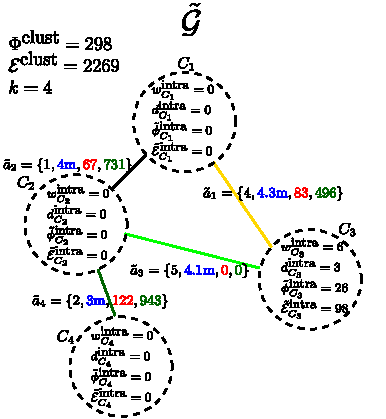
\includegraphics[width=0.45\linewidth]{Images/G_4.pdf}
    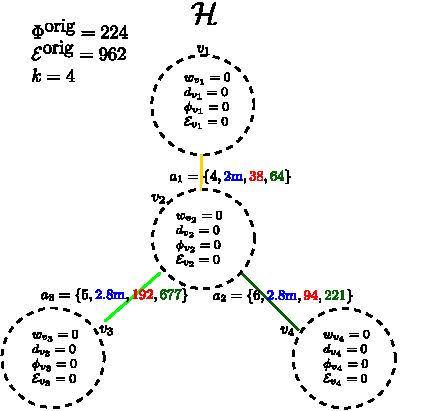
\includegraphics[width=0.48\linewidth]{Images/H.pdf}\\
    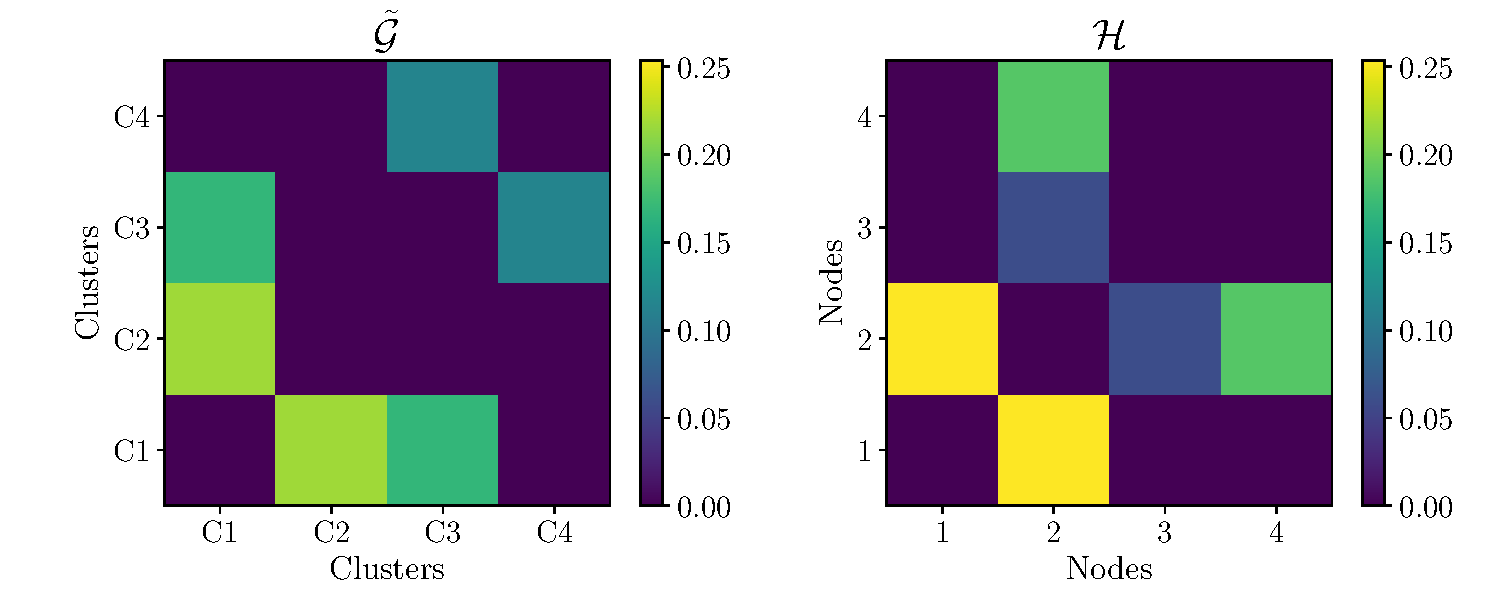
\includegraphics[width=1.0\linewidth]{Images/ae_graphon_comparison.pdf}
    \caption{Kernel graph process with $k=4$}
    \label{fig:ae_kernel}
\end{figure}

% \subsection{Network Comparison via Gromov-Wasserstein}
% Given $\mathcal{G}$ (Paris) and $\mathcal{H}$ (Grenoble) with $|\mathcal{V}^\mathcal{G}| > |\mathcal{V}^\mathcal{H}|$:
% \begin{enumerate}
%     \item Cluster $\mathcal{G}$ to $\tilde{\mathcal{G}}$ with $|\tilde{\mathcal{V}}| = |\mathcal{V}^\mathcal{H}|$ (Algorithm~\ref{alg:constrained-clustering-math}).
%     \item Define node exposure distributions $\mu_\mathcal{E}^{\tilde{\mathcal{G}}}$, $\mu_\mathcal{E}^\mathcal{H}$ as in \eqref{node_exposure_def}.
%     \item Compute $GW_2(\tilde{\mathcal{G}}, \mathcal{H})$ via \eqref{gw_distance}.
% \end{enumerate}

% \begin{algorithm}[H]
% \caption{Constrained Spectral Clustering for Bike Networks (Short Version)}
% \label{alg:constrained-clustering-short}
% \begin{algorithmic}[1]
% \Require Graph $\mathcal{G}=(\mathcal{V},\mathcal{A},\mathcal{W})$, number of clusters $k$, parameters $\epsilon_{\max}$, $\delta_{\max}$, $\Delta\mathcal{E}_{\max}$, $\Delta\Phi_{\max}$, $\alpha_{\text{relax}}$
% \Ensure Clustered graph $\tilde{\mathcal{G}}=(\tilde{\mathcal{V}},\tilde{\mathcal{A}},\tilde{\mathcal{W}})$

% \State \textbf{Spectral Embedding:}
%     Compute $A$ and $L$ as above; extract $m$ leading eigenvectors to form embedding $\mathbf{X}$.

% \State \textbf{Initialize Constraints:}
%     $\tau_{\mathcal{E}} \gets \Delta\mathcal{E}_{\max}$, $\tau_{\Phi} \gets \Delta\Phi_{\max}$

% \For{$attempt = 1$ to $max\_attempts$}
%     \State Run constrained k-means on $\mathbf{X}$:
%         \begin{itemize}
%             \item Assign $v_i$ to $C_p$ minimizing squared distance plus penalties for DoS or distance violations.
%             \item Constraints: 
%             $\max_{v_j \in C_p} |w_{ij} - \min w_{ij}| \leq \epsilon_{\max}$,
%             $\max_{v_j \in C_p} d_{ij} \leq \delta_{\max}$.
%         \end{itemize}
%     \State Build $\tilde{\mathcal{G}}$ with weights from Section~\ref{section_flows}.
%     \State Compute $\mathcal{E}_{\text{clust}}$ and $\Phi_{\text{clust}}$.
%     \State $\Delta\mathcal{E} \gets |\mathcal{E}_{\text{orig}} - \mathcal{E}_{\text{clust}}|$, \quad
%           $\Delta\Phi \gets |\Phi_{\text{orig}} - \Phi_{\text{clust}}|$.
%     \If{$\Delta\mathcal{E} \leq \tau_{\mathcal{E}}$ \textbf{and} $\Delta\Phi \leq \tau_{\Phi}$}
%         \State \Return $\tilde{\mathcal{G}}$
%     \Else
%         \State Relax tolerances: 
%         $\tau_{\mathcal{E}} \gets \tau_{\mathcal{E}} \cdot \alpha_{\text{relax}}$, \;
%         $\tau_{\Phi} \gets \tau_{\Phi} \cdot \alpha_{\text{relax}}$
%     \EndIf
% \EndFor

% \State \textbf{Fallback:} If no feasible clustering is found, run unconstrained k-means and return with warning.
% \end{algorithmic}
% \end{algorithm}




% \begin{algorithm}[H]
% \caption{Constrained spectral $k$-means clustering for cycling networks}
% \label{alg:constrained-clustering-math}
% \begin{algorithmic}[1]
% \Require 
%   $\mathcal{G} = (\mathcal{V}, \mathcal{A}, \mathcal{W})$; 
%   $k$; 
%   $\epsilon_{\max}$ (DoS tolerance); 
%   $\delta_{\max}$ (spatial tolerance); 
%   $\tau_{\mathcal{E}}^{(0)}$, $\tau_{\Phi}^{(0)}$ (initial exposure/flow tolerances); 
%   $\alpha_{\text{relax}}>1$; 
%   $\lambda_1,\lambda_2$; 
%   $T_{\max}$.
% \Ensure Clustered graph $\tilde{\mathcal{G}} = (\mathcal{C}, \tilde{\mathcal{A}}, \tilde{\mathcal{W}})$, $\mathcal{C}=\{C_1,\dots,C_k\}$.

% \State \textbf{Spectral embedding:} build
% \[
% A_{ij} =
% \begin{cases}
% w_{ij}\,\exp(-d_{ij}/\gamma)\Bigl(\dfrac{\phi_{ij}}{\max \phi}\Bigr)^{\alpha}, & (i,j)\in\mathcal{A},\\[0.3em]
% 0, & \text{otherwise},
% \end{cases}
% \quad
% \mathcal{L} = I - D^{-1/2} A D^{-1/2},\ D_{ii}=\sum_j A_{ij}.
% \]
% Compute the first $m$ eigenvectors of $\mathcal{L}$, stack them row-wise into $\mathbf{X}\in\mathbb{R}^{|\mathcal{V}|\times m}$.

% \State Compute original totals $\Phi^{\mathrm{orig}},\ \mathcal{E}^{\mathrm{orig}}$ from \eqref{eq_flows} and \eqref{exposure_def}.
% \State Set $\tau_{\mathcal{E}} \gets \tau_{\mathcal{E}}^{(0)}$, \quad $\tau_{\Phi} \gets \tau_{\Phi}^{(0)}$.

% \For{$t = 1,\dots,T_{\max}$}
%   \State Initialize centroids $\{\mu_r\}_{r=1}^k$ (e.g., $k$-means++ on $\mathbf{X}$).
%   \State \textbf{Constrained assignment:} for each node $v_i$ with embedding $\mathbf{x}_i$, choose
%   \[
%   r^* 
%   = 
%   \arg\min_{r\in\{1,\dots,k\}}
%   \Bigl\{
%     \|\mathbf{x}_i - \mu_r\|^2
%     + \lambda_1\,\mathbb{I}_{\mathrm{DoSViol}}(i,r)
%     + \lambda_2\,\mathbb{I}_{\mathrm{DistViol}}(i,r)
%   \Bigr\},
%   \]
%   where $\mathbb{I}_{\mathrm{DoSViol}}(i,r)$ (resp.\ $\mathbb{I}_{\mathrm{DistViol}}(i,r)$) equals $1$ if assigning $v_i$ to $C_r$ would violate
%   \[
%     \max_{v_j\in C_r} |w_{ij} - \min_{v_\ell\in C_r} w_{i\ell}| \le \epsilon_{\max},
%     \qquad
%     \max_{v_j\in C_r} d_{ij} \le \delta_{\max},
%   \]
%   and $0$ otherwise. Set $v_i \mapsto C_{r^*}$ and update
%   \[
%     \mu_r \gets \frac{1}{|C_r|}\sum_{v_j\in C_r}\mathbf{x}_j \quad \forall r.
%   \]

%   \State Build $\tilde{\mathcal{G}} = (\mathcal{C},\tilde{\mathcal{A}},\tilde{\mathcal{W}})$ from $\{C_r\}$ using the inter-/intra-cluster definitions in 
%   Sections~\ref{sec:clustered-distance}--\ref{sec:clustered-flows}, and compute $\Phi^{\mathrm{clust}},\ \mathcal{E}^{\mathrm{clust}}$ from \eqref{cluster_def}.

%   \State Evaluate deviations
%   \[
%     \Delta\mathcal{E} = \bigl|\mathcal{E}^{\mathrm{orig}} - \mathcal{E}^{\mathrm{clust}}\bigr|,
%     \qquad
%     \Delta\Phi = \bigl|\Phi^{\mathrm{orig}} - \Phi^{\mathrm{clust}}\bigr|.
%   \]

%   \If{$\Delta\mathcal{E} \le \tau_{\mathcal{E}}$ \textbf{ and } $\Delta\Phi \le \tau_{\Phi}$}
%     \State \Return $\tilde{\mathcal{G}}$ \Comment{constraints satisfied}
%   \Else
%     \State $\tau_{\mathcal{E}} \gets \alpha_{\text{relax}}\,\tau_{\mathcal{E}}$, \quad
%            $\tau_{\Phi} \gets \alpha_{\text{relax}}\,\tau_{\Phi}$ \Comment{progressive relaxation}
%   \EndIf
% \EndFor

% \State \textbf{Fallback:} run unconstrained $k$-means on $\mathbf{X}$, build $\tilde{\mathcal{G}}$ from the resulting clusters, and \Return $\tilde{\mathcal{G}}$.
% \end{algorithmic}
% \end{algorithm}


% \begin{algorithm}[H]
% \caption{Constrained spectral $k$-means clustering for cycling networks}
% \label{alg:constrained-clustering-math}
% \begin{algorithmic}[1]
% \Require 
%   $\mathcal{G} = (\mathcal{V}, \mathcal{A}, \mathcal{W})$; 
%   $k$; 
%   $\epsilon_{\max}$; 
%   $\delta_{\max}$; 
%   $\tau_{\mathcal{E}}^{(0)}$, $\tau_{\Phi}^{(0)}$ ; 
%   $\alpha_{\text{relax}}>1$; 
%   $\lambda_1,\lambda_2$; 
%   $T_{\max}$.
% \Ensure Clustered graph $\tilde{\mathcal{G}} = (\mathcal{C}, \tilde{\mathcal{A}}, \tilde{\mathcal{W}})$, $\mathcal{C}=\{C_1,\dots,C_k\}$.

% \State \textbf{Spectral embedding:} build
% \[
% A_{ij} =
% \begin{cases}
% w_{ij}\,\exp(-d_{ij}/\gamma)\Bigl(\dfrac{\phi_{ij}}{\max \phi}\Bigr)^{\alpha}, & (i,j)\in\mathcal{A},\\[0.3em]
% 0, & \text{otherwise},
% \end{cases}
% \quad
% \mathcal{L} = I - D^{-1/2} A D^{-1/2},\ D_{ii}=\sum_j A_{ij}.
% \]
% Compute the first $m$ eigenvectors of $\mathcal{L}$, stack them row-wise into $\mathbf{X}\in\mathbb{R}^{|\mathcal{V}|\times m}$.

% \State Compute original totals $\Phi^{\mathrm{orig}},\ \mathcal{E}^{\mathrm{orig}}$ from \eqref{eq_flows} and \eqref{exposure_def}.
% \State Set $\tau_{\mathcal{E}} \gets \tau_{\mathcal{E}}^{(0)}$, \quad $\tau_{\Phi} \gets \tau_{\Phi}^{(0)}$.

% \For{$t = 1,\dots,T_{\max}$}
%   \State Initialize centroids $\{\mu_r\}_{r=1}^k$ (e.g., $k$-means++ on $\mathbf{X}$).
%   \State \textbf{Constrained assignment:} for each node $v_i$ with embedding $\mathbf{x}_i$, choose
%   \[
%   r^* 
%   = 
%   \arg\min_{r\in\{1,\dots,k\}}
%   \Bigl\{
%     \|\mathbf{x}_i - \mu_r\|^2
%     + \lambda_1\,\mathbb{I}_{\mathrm{DoSViol}}(i,r)
%     + \lambda_2\,\mathbb{I}_{\mathrm{DistViol}}(i,r)
%   \Bigr\},
%   \]
%   where $\mathbb{I}_{\mathrm{DoSViol}}(i,r)$ (resp.\ $\mathbb{I}_{\mathrm{DistViol}}(i,r)$) equals $1$ if assigning $v_i$ to $C_r$ would violate
%   \[
%     \max_{v_j\in C_r} |w_{ij} - \min_{v_\ell\in C_r} w_{i\ell}| \le \epsilon_{\max},
%     \qquad
%     \max_{v_j\in C_r} d_{ij} \le \delta_{\max},
%   \]
%   and $0$ otherwise. Set $v_i \mapsto C_{r^*}$ and update
%   \[
%     \mu_r \gets \frac{1}{|C_r|}\sum_{v_j\in C_r}\mathbf{x}_j \quad \forall r.
%   \]

%   \State Build $\tilde{\mathcal{G}} = (\mathcal{C},\tilde{\mathcal{A}},\tilde{\mathcal{W}})$ from $\{C_r\}$ using the inter-/intra-cluster definitions in 
%   Sections~\ref{sec:clustered-distance}--\ref{sec:clustered-flows}, and compute $\Phi^{\mathrm{clust}},\ \mathcal{E}^{\mathrm{clust}}$ from \eqref{cluster_def}.

%   \State Evaluate deviations
%   \[
%     \Delta\mathcal{E} = \bigl|\mathcal{E}^{\mathrm{orig}} - \mathcal{E}^{\mathrm{clust}}\bigr|,
%     \qquad
%     \Delta\Phi = \bigl|\Phi^{\mathrm{orig}} - \Phi^{\mathrm{clust}}\bigr|.
%   \]

%   \If{$\Delta\mathcal{E} \le \tau_{\mathcal{E}}$ \textbf{ and } $\Delta\Phi \le \tau_{\Phi}$}
%     \State \Return $\tilde{\mathcal{G}}$ \Comment{constraints satisfied}
%   \Else
%     \State $\tau_{\mathcal{E}} \gets \alpha_{\text{relax}}\,\tau_{\mathcal{E}}$, \quad
%            $\tau_{\Phi} \gets \alpha_{\text{relax}}\,\tau_{\Phi}$ \Comment{progressive relaxation}
%   \EndIf
% \EndFor

% \State \textbf{Fallback:} run unconstrained $k$-means on $\mathbf{X}$, build $\tilde{\mathcal{G}}$ from the resulting clusters, and \Return $\tilde{\mathcal{G}}$.
% \end{algorithmic}
% \end{algorithm}



\section{Case Study}



\begin{figure*}
    \centering
    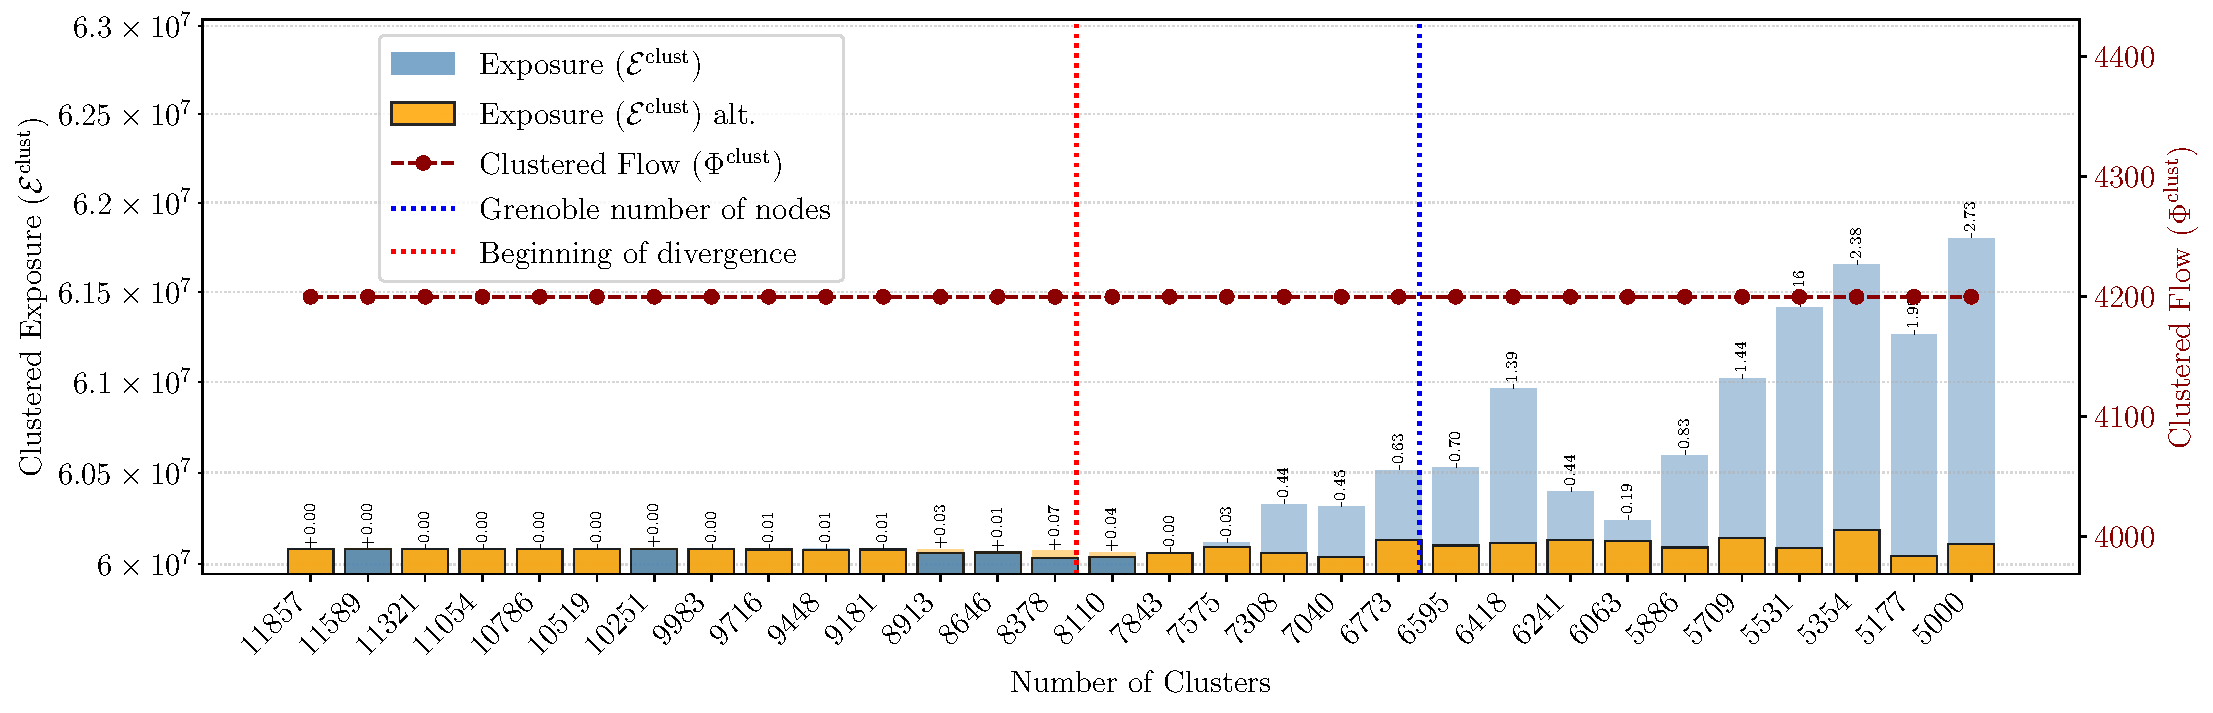
\includegraphics[width=2\columnwidth]{Images/clustered_expo_flow_overlap_log_Lyon_divergence.pdf}\\
    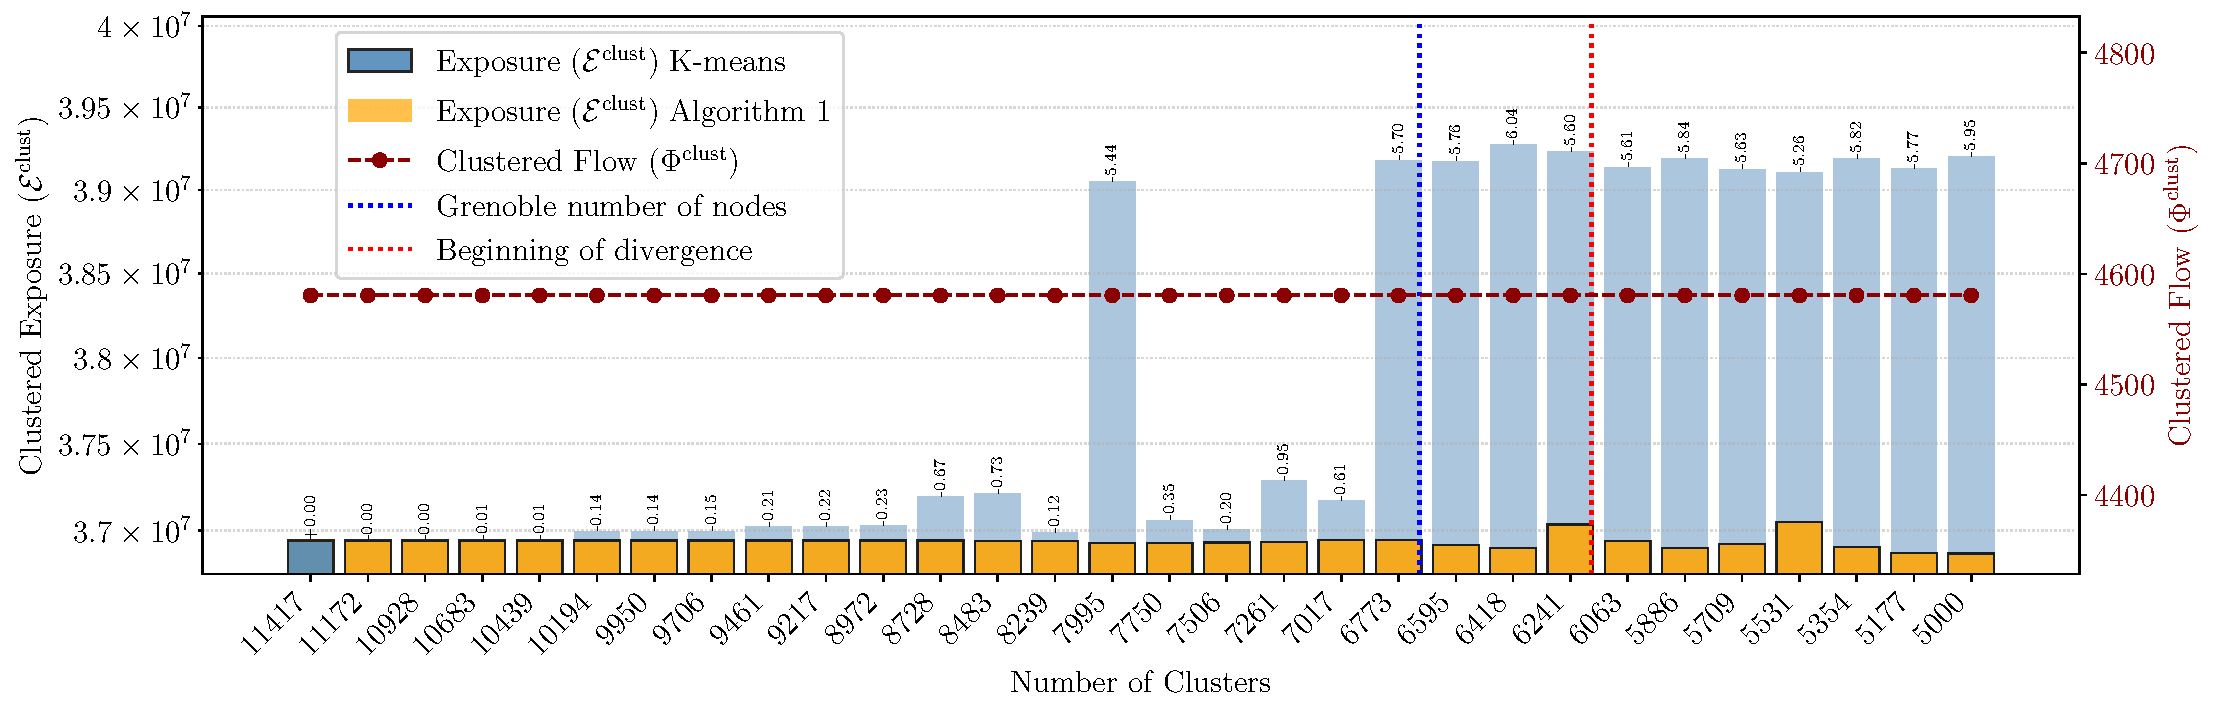
\includegraphics[width=2\columnwidth]{Images/clustered_expo_flow_overlap_log_Strasbourg_divergence.pdf}
    \caption{Evolution of cyclist exposure and cyclist flow through the Algorithm A, on the top Lyon and on the bottom Strasbourg case.}
    \label{fig:exposure_comparison}
\end{figure*}

\begin{figure*}[t]
\centering
\captionsetup[subfigure]{font={footnotesize}, labelfont={footnotesize, bf}, textfont={footnotesize, rm}}
\subfloat[Original]{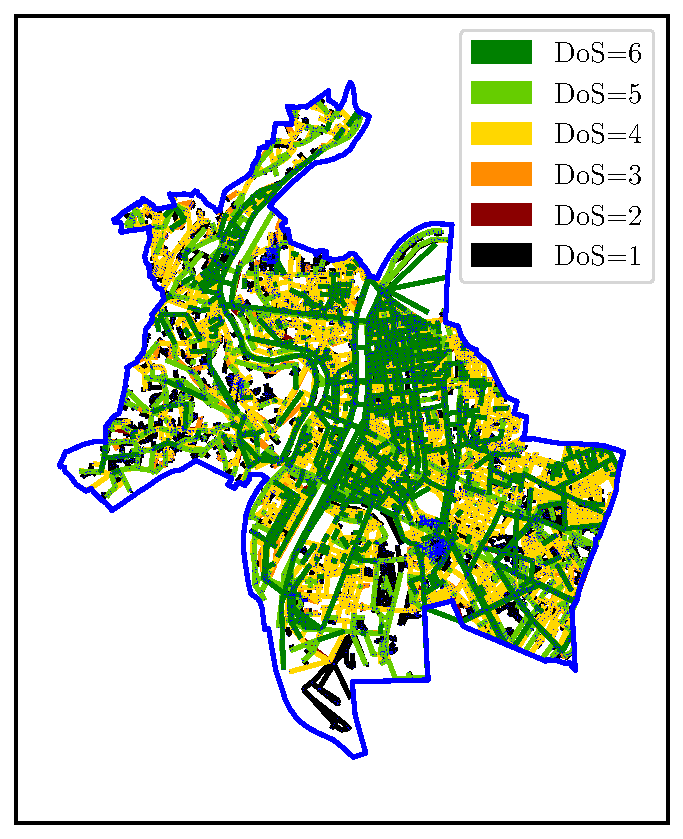
\includegraphics[width=0.480\columnwidth]{Images/Lyon_DoS_1.pdf}}
\subfloat[$K$-mean]{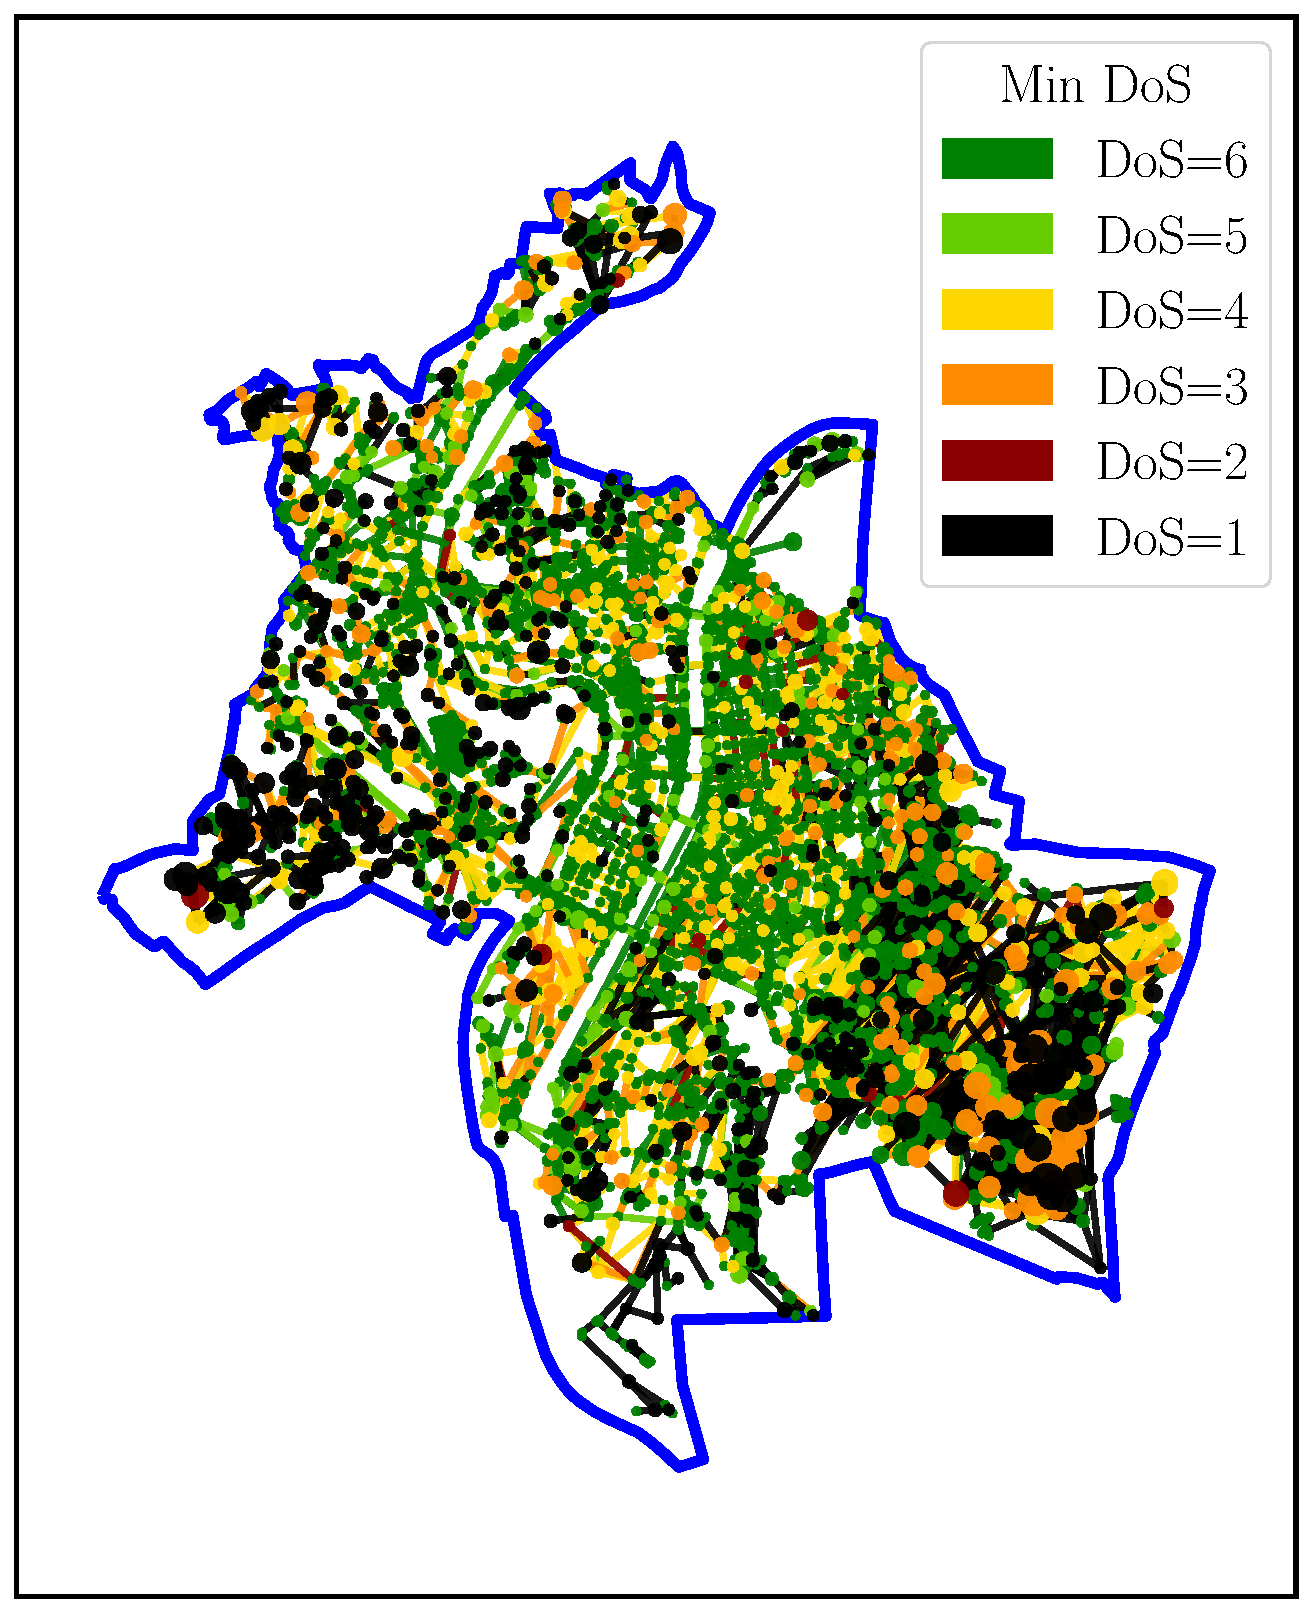
\includegraphics[width=0.48\columnwidth]{Images/H_clust_by_key_Lyon_algorithm.pdf}}
\subfloat[Algorithm 1]{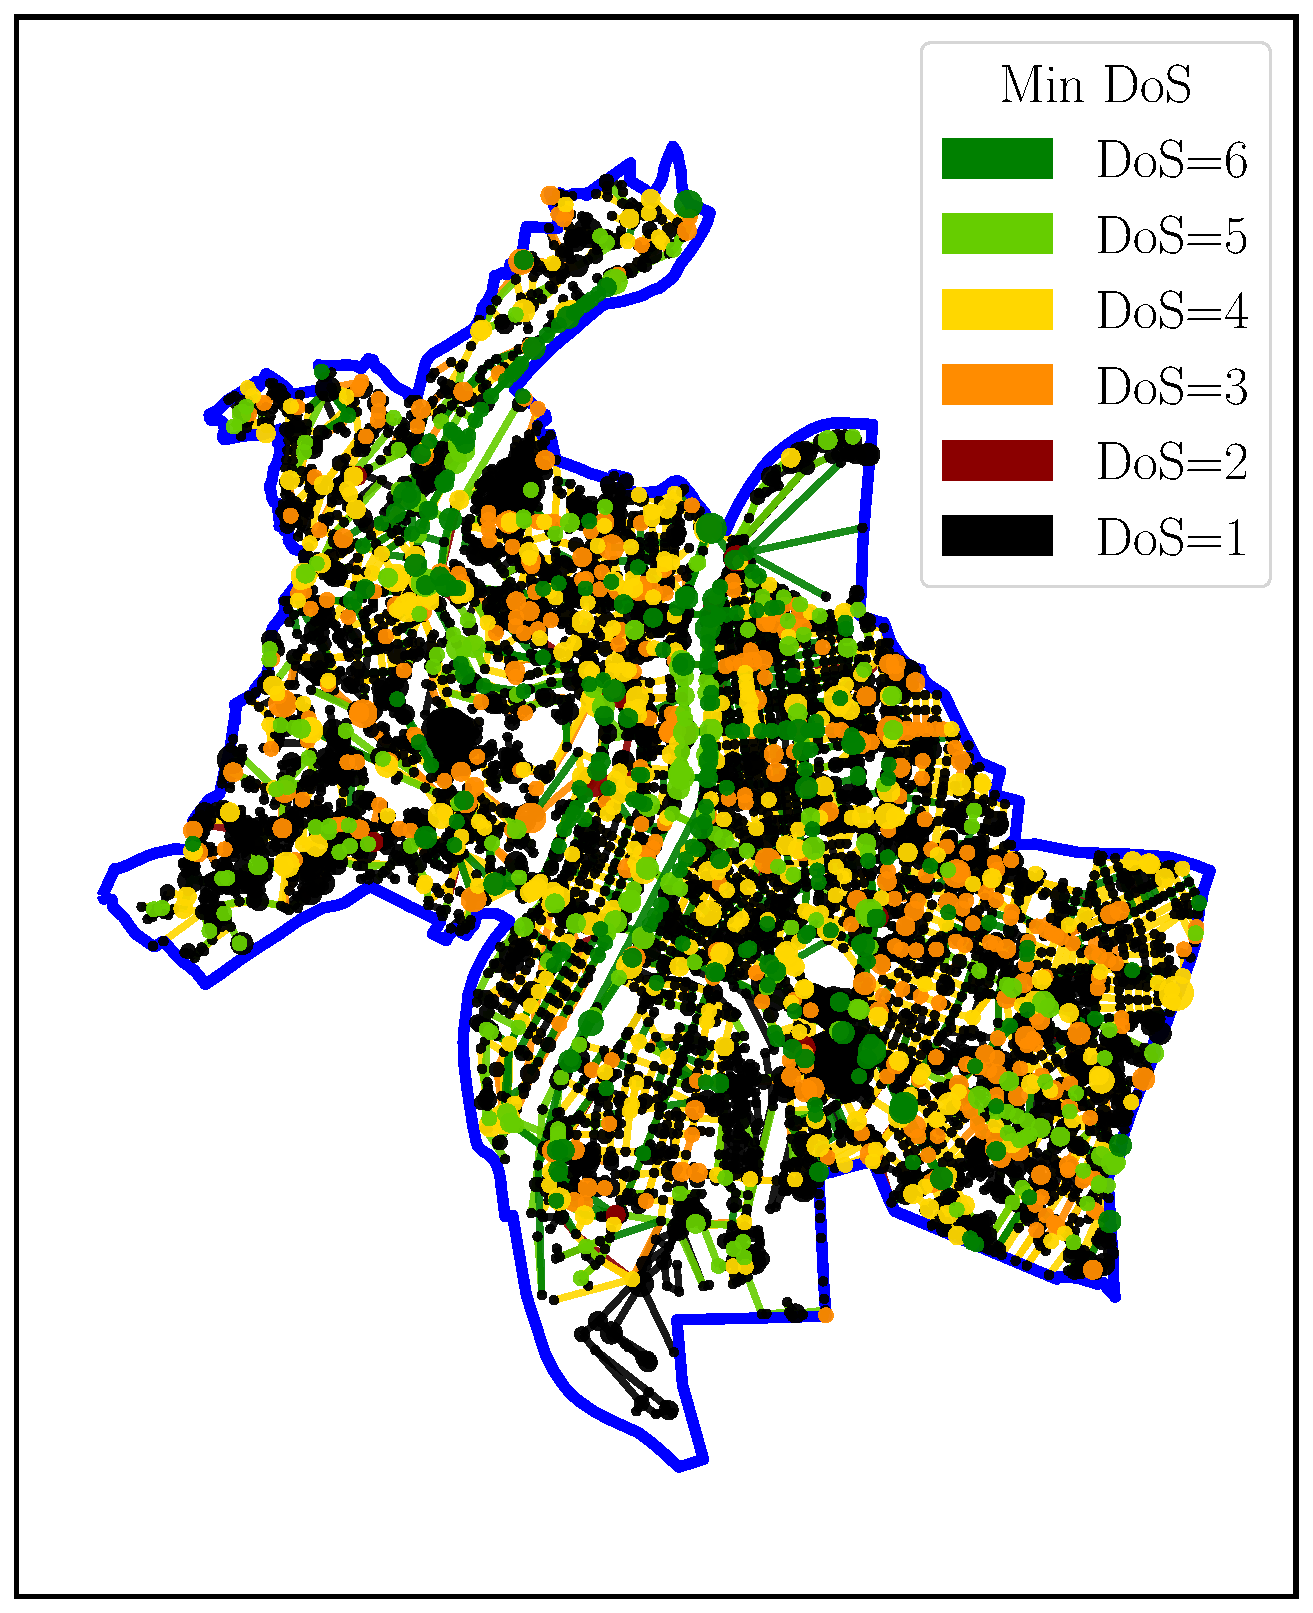
\includegraphics[width=0.48\columnwidth]{Images/H_clust_by_key_Lyon.pdf}}\\
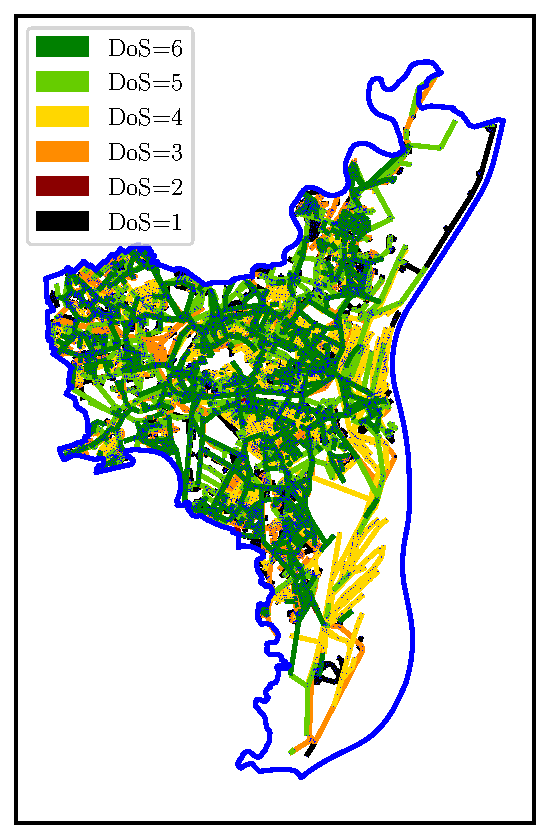
\includegraphics[width=0.480\columnwidth]{Images/Strasbourg_DoS_1.pdf}
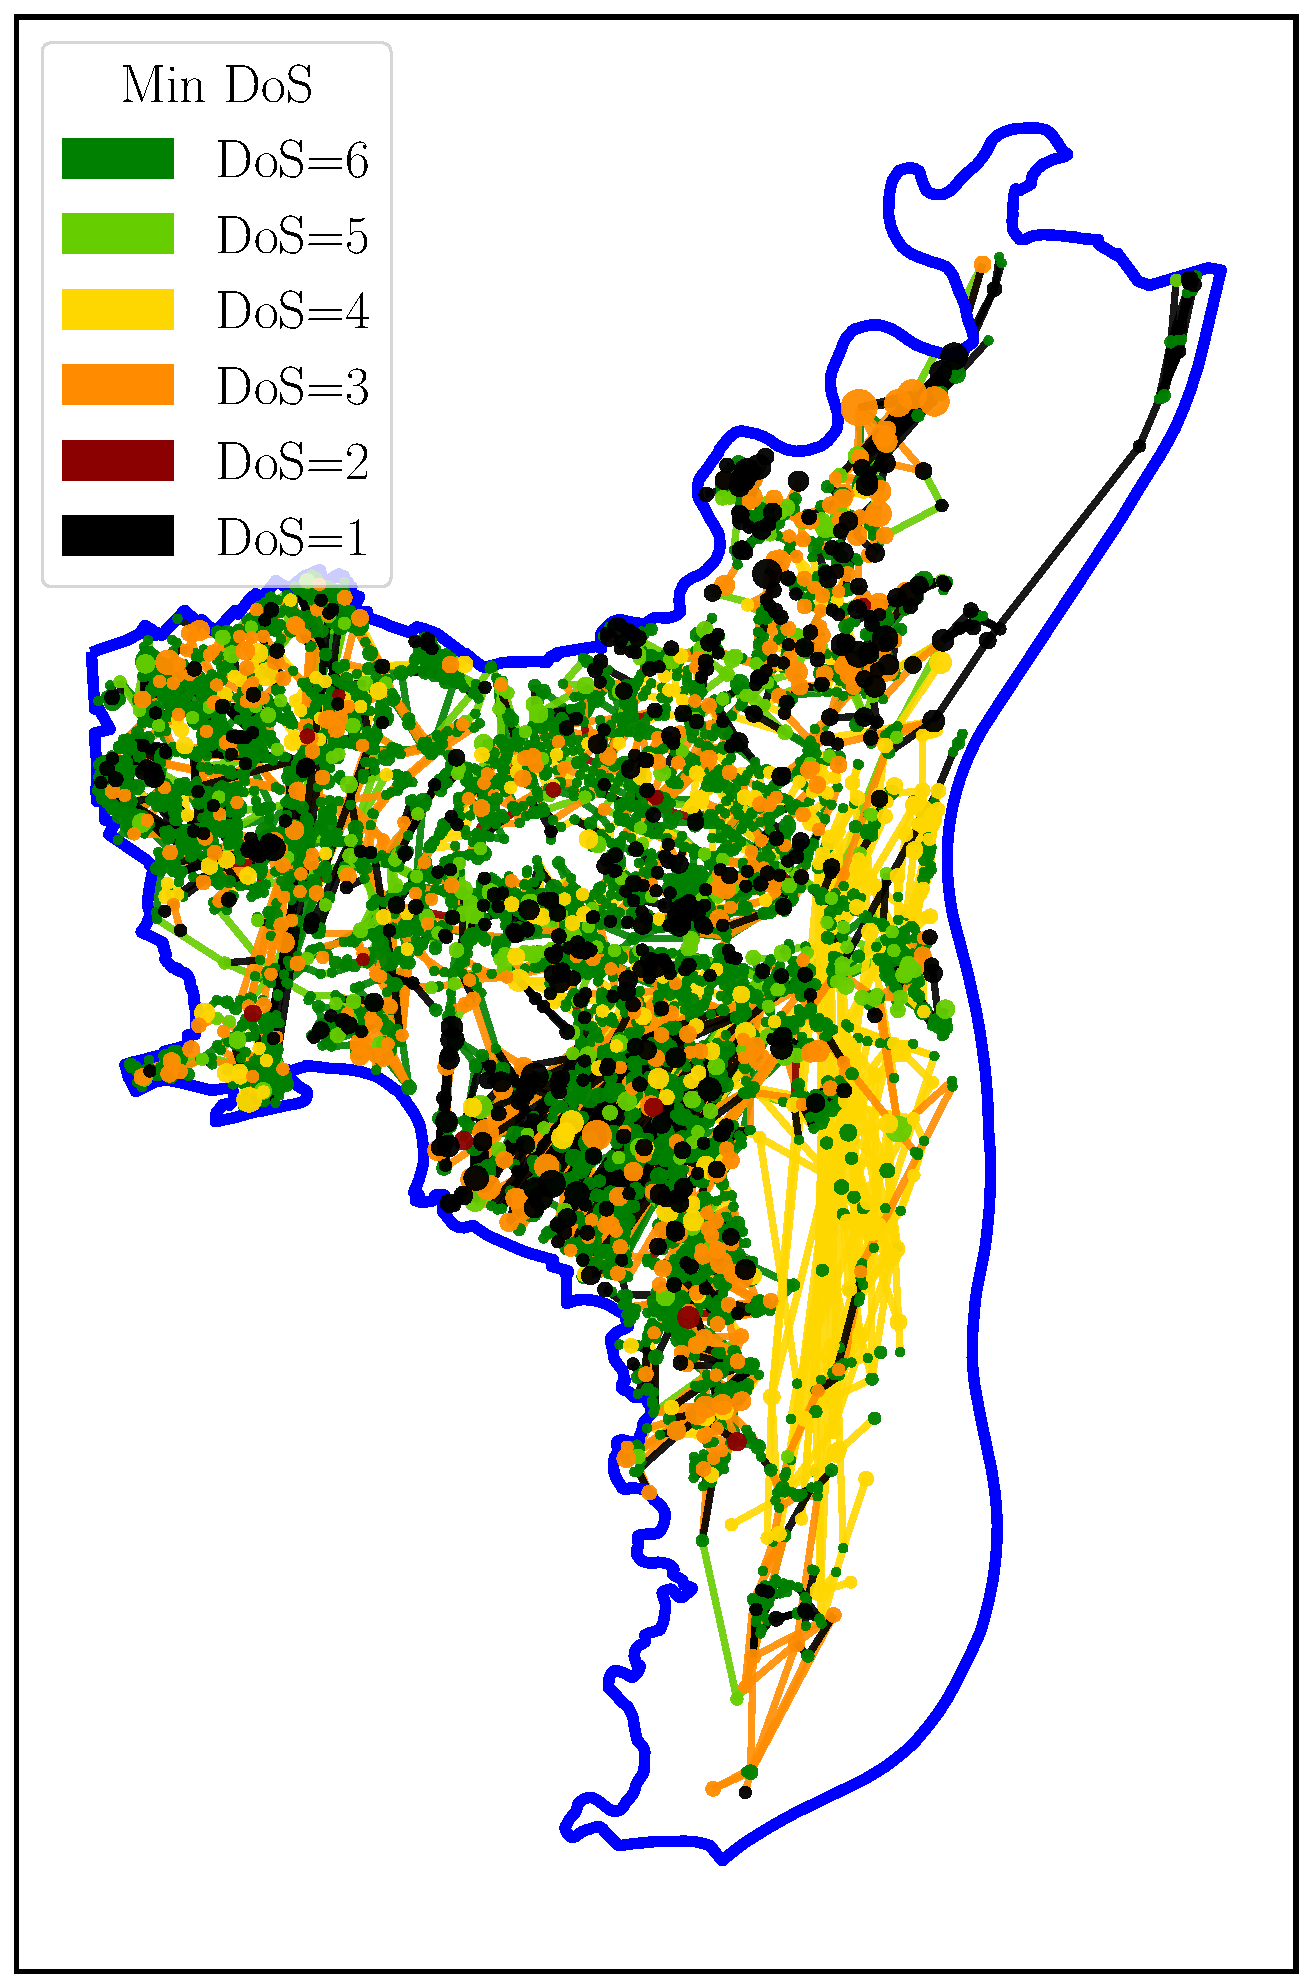
\includegraphics[width=0.48\columnwidth]{Images/H_clust_by_key_strasbourg_algorithm.pdf}
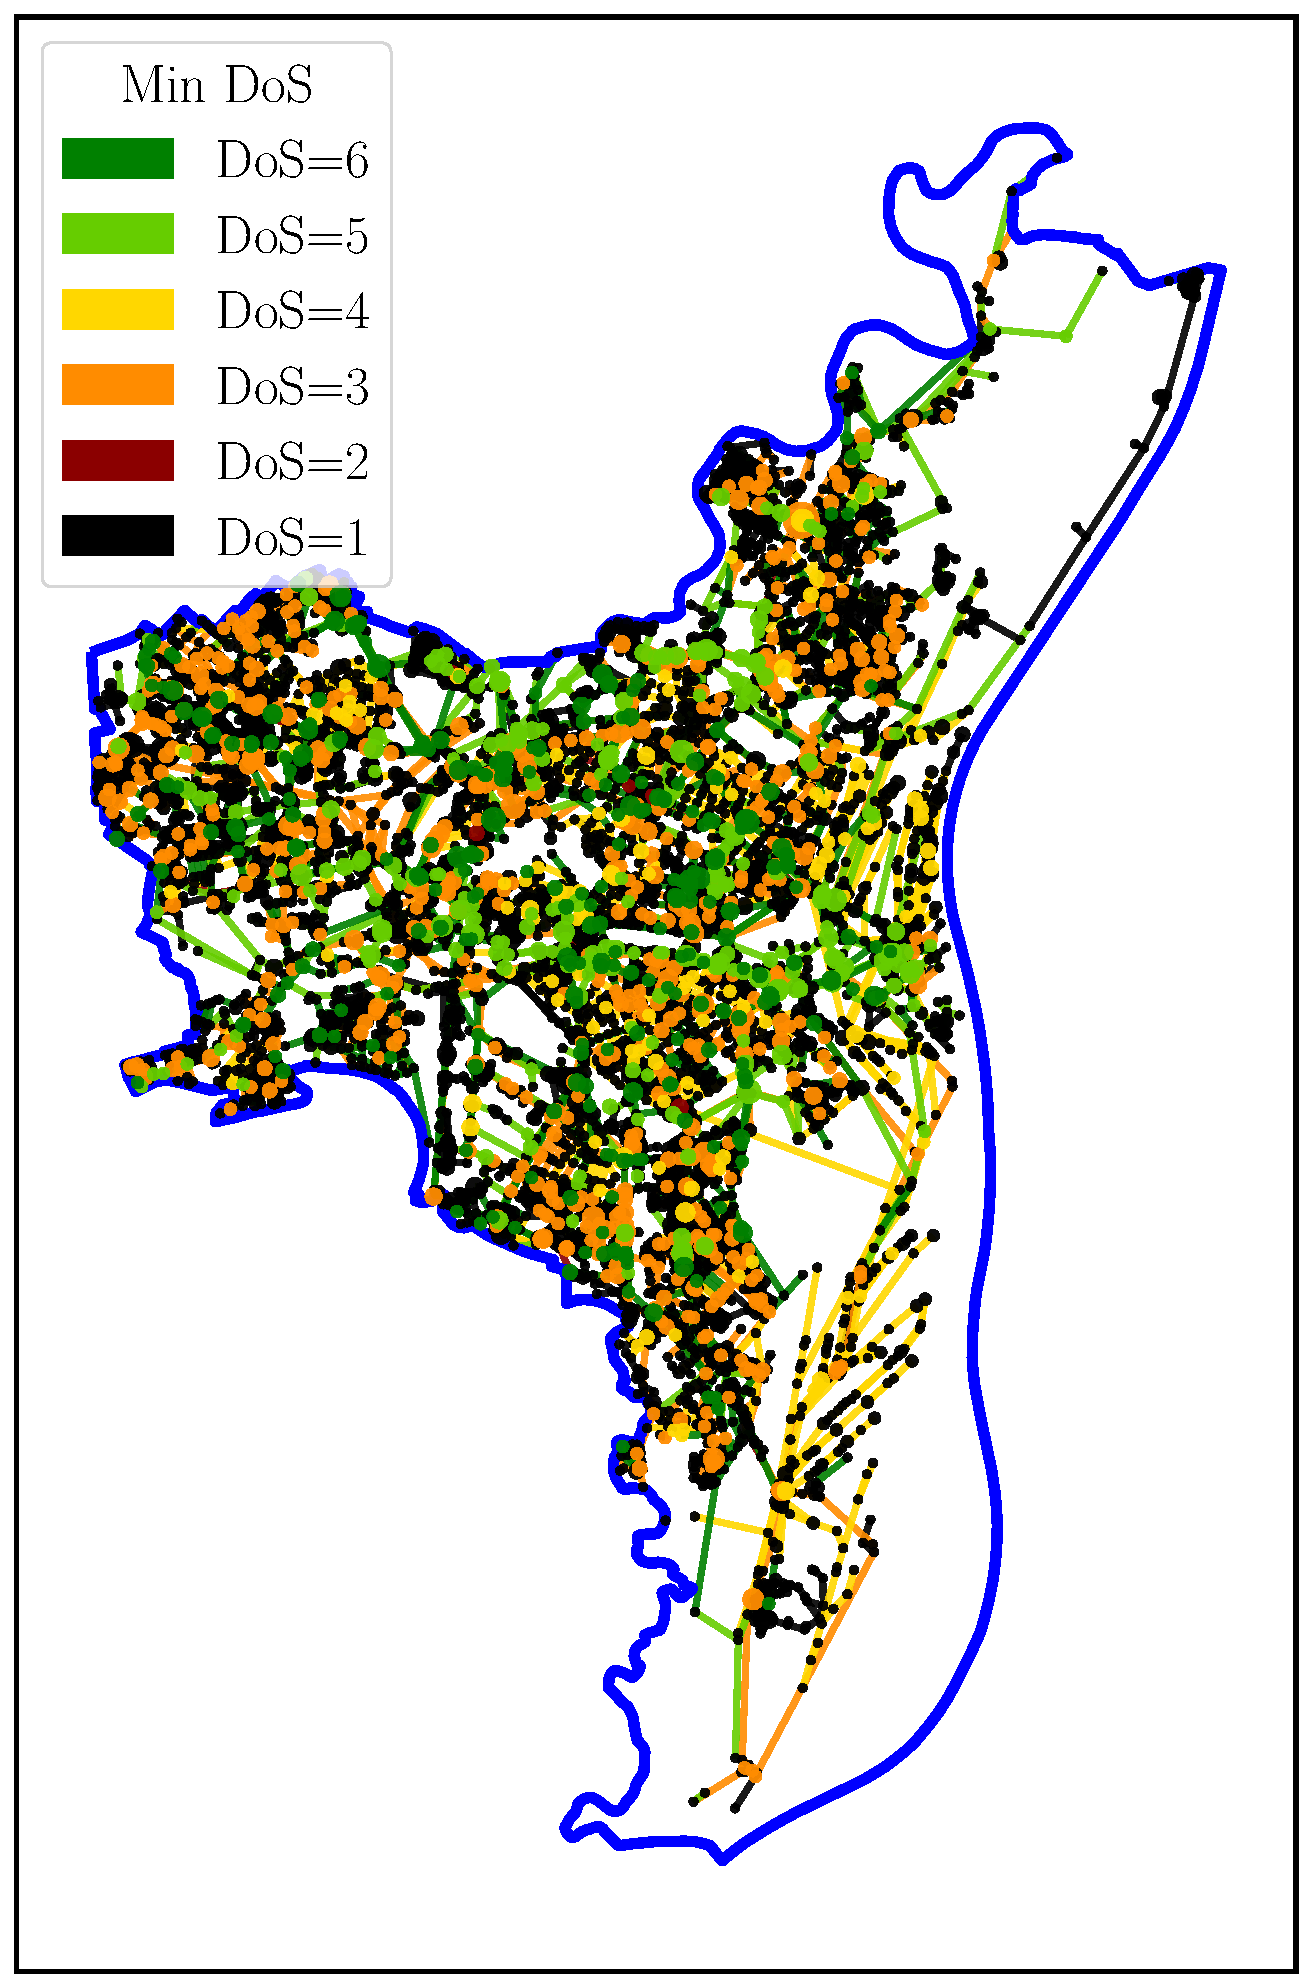
\includegraphics[width=0.48\columnwidth]{Images/H_clust_by_key_strasbourg.pdf}
\caption{\footnotesize Clustering process with Algorithm 1, on the first column we have the original networks, then the cluster one with $K$-mean and finally with Algorithm 1.}
\label{fig:cluster_comparison_topology}
\end{figure*}

\begin{figure}
    \centering
    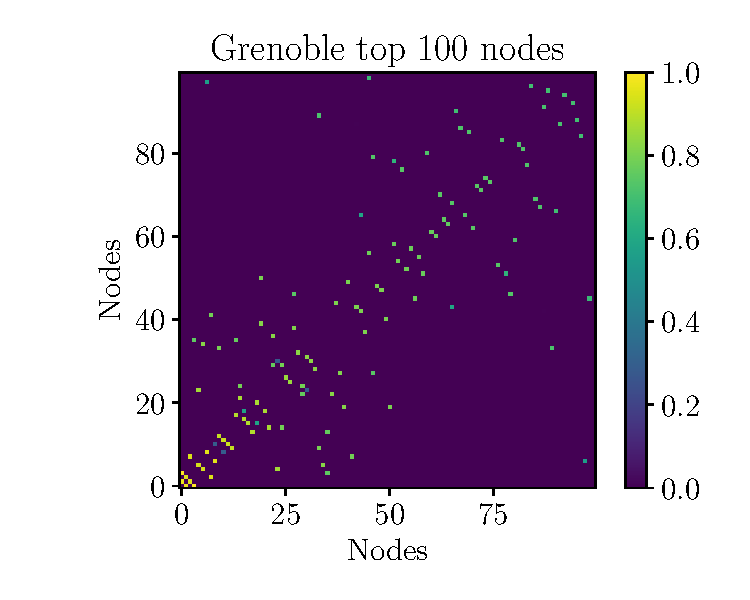
\includegraphics[width=1\columnwidth]{Images/top_100_kernel_log_Grenoble.pdf}
    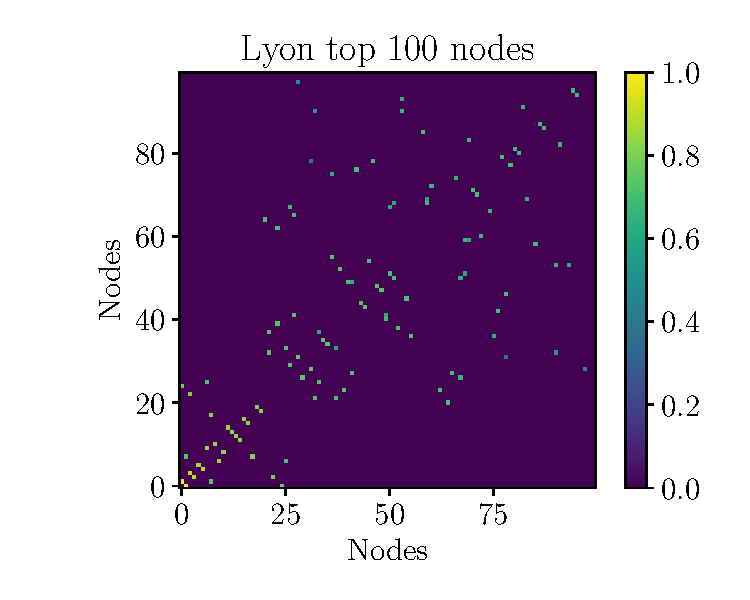
\includegraphics[width=1\columnwidth]{Images/top_100_kernel_log_Lyon.pdf}
    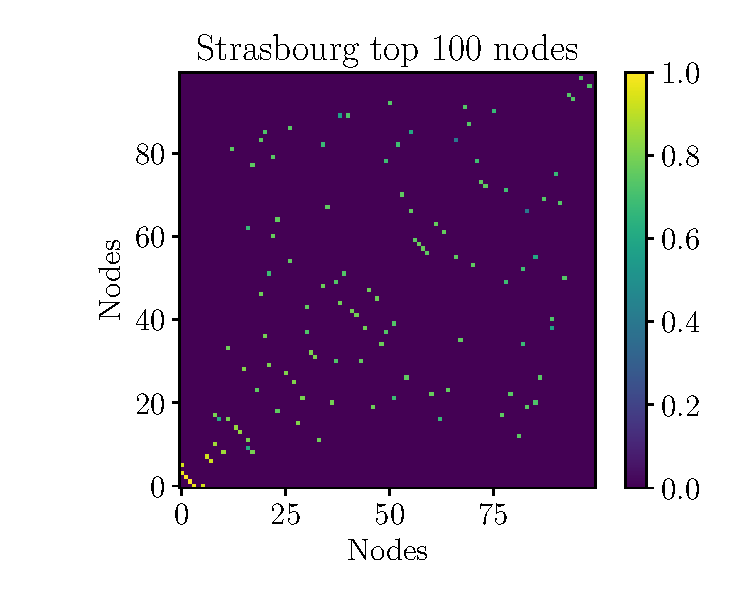
\includegraphics[width=1\columnwidth]{Images/top_100_kernel_log_Strasbourg.pdf}
    \caption{Heatmaps of top 100 nodes kernels comparison between Grenoble, Lyon and Strasbourg.}
    \label{fig:exposure_evolution_heat_map}
\end{figure}


\begin{figure*}
    \centering
    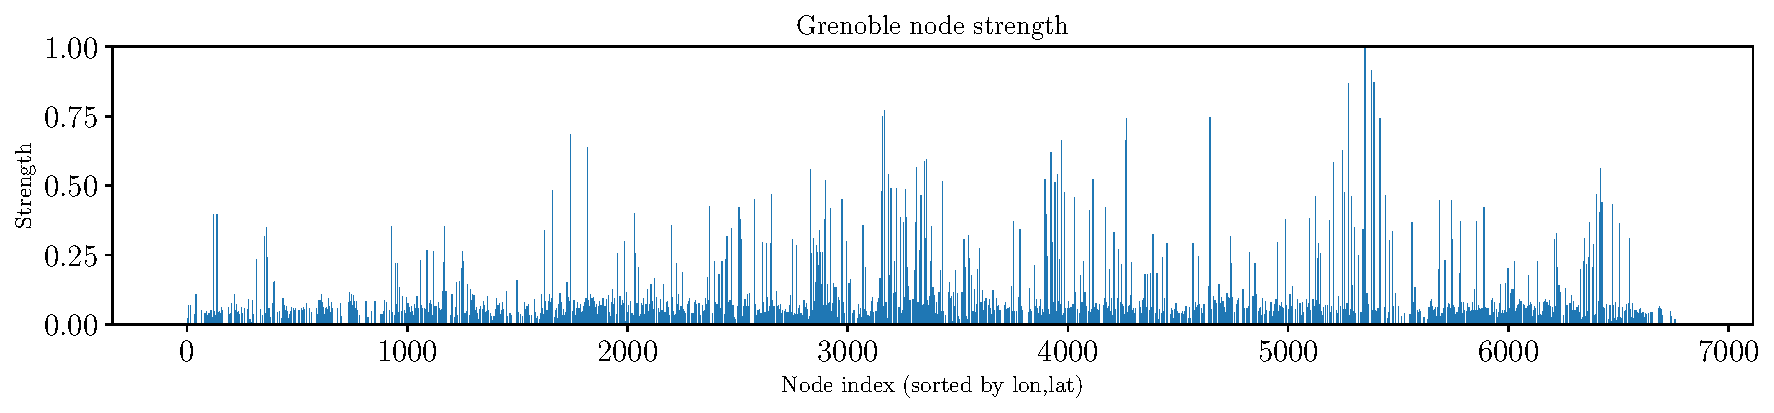
\includegraphics[width=2\columnwidth]{Images/strength_bars_Grenoble.pdf}\\
    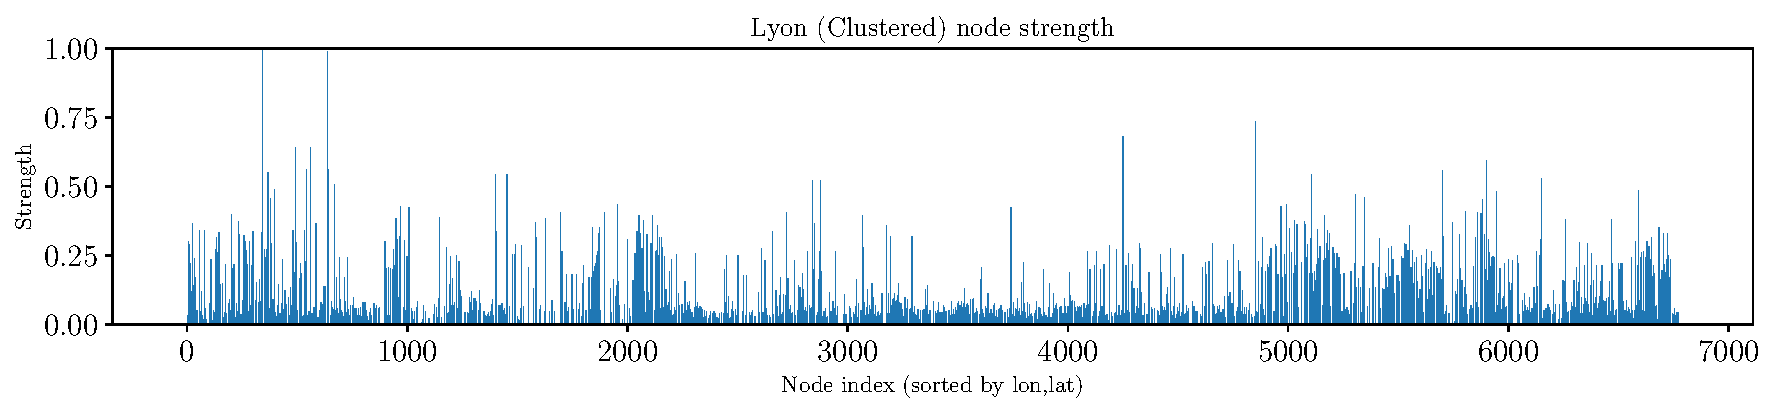
\includegraphics[width=2\columnwidth]{Images/strength_bars_Lyon.pdf}\\
    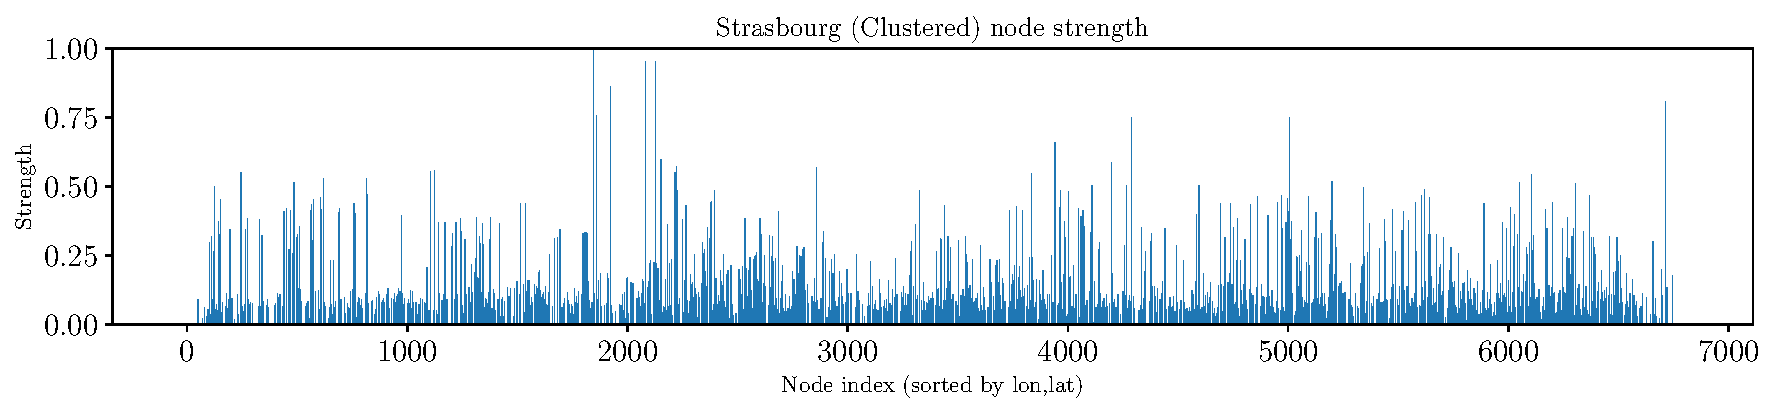
\includegraphics[width=2\columnwidth]{Images/strength_bars_Strasbourg.pdf}
    \caption{Node strength of Grenoble and clustered Lyon and Strasbourg cycling networks.}
    \label{fig:node_strength_distribution}
\end{figure*}

We illustrate the proposed framework on three French cities with well-developed cycling networks:
Lyon ($11\,857$ nodes), Strasbourg ($11\,417$ nodes), and Grenoble ($6\,773$ nodes).  
Grenoble is the smallest network and is taken as the reference.  
For each of the larger cities, we apply Algorithm~1 to cluster their network down to $|\mathcal{C}| = 6\,773$ supernodes, yielding clustered networks $\tilde{\mathcal{G}}^{\mathrm{Lyon}}$ and $\tilde{\mathcal{G}}^{\mathrm{Strasbourg}}$ that are comparable in size to $\mathcal{H}^{\mathrm{Grenoble}}$.
We then compare each clustered network to Grenoble using the Wasserstein and kernel–graphon metrics introduced in Section~\ref{sec:gw_comparison}.


Figure~\ref{fig:exposure_comparison} shows how the total clustered exposure $\mathcal{E}^{\mathrm{clust}}$ (bars, left axis) and total clustered flow $\Phi^{\mathrm{clust}}$ (red dashed line, right axis) evolve as the number of clusters decreases, for Lyon (top) and Strasbourg (bottom).  
The blue vertical line marks the point where the number of clusters equals the number of Grenoble nodes ($6\,773$), while the red vertical line indicates the onset of noticeable divergence between the original and clustered exposure. Two clustering strategies are compared: unconstrained $k$-means and Algorithm~1.  
Across both cities, Algorithm~1 consistently produces clustered networks whose total exposure remains much closer to the original value, particularly in the high-compression regime (towards the right of the plots).  
Lyon reaches the divergence threshold earlier: once the number of clusters falls below about $6\,200$, the exposure under $k$-means and (to a lesser extent) Algorithm~1 deviates more strongly from the original network.  
In contrast, Strasbourg maintains a near-constant exposure over a wider range of cluster counts, suggesting that its DoS structure can be compressed more aggressively without losing safety-relevant information.  
The clustered flow remains remarkably stable under Algorithm~1, confirming that the total cyclist demand is well preserved during clustering.

Figure~\ref{fig:cluster_comparison_topology} compares the spatial distribution of the degree of separation before and after clustering, for Lyon (top row) and Strasbourg (bottom row).  
The first column shows the original networks coloured by DoS, the second the result of unconstrained $k$-means, and the third the result of Algorithm~1. While both methods reduce the number of nodes to match Grenoble, the unconstrained $k$-means clustering tends to mix arcs of very different DoS within the same cluster, leading to patches where risky and safe segments are aggregated and the minimum DoS is not systematically preserved. Algorithm~1, by construction, assigns to each cluster the worst (minimum) DoS of its constituent arcs and enforces bounds on intra-cluster DoS and spatial diameter. Visually, this yields clustered networks whose high-risk corridors and low-risk greenways remain clearly aligned with those of the original networks, even under substantial node reduction. This qualitative behaviour is consistent with the exposure and flow curves in Figure~\ref{fig:exposure_comparison}.

To inspect the exposure structure more locally, Figure~\ref{fig:exposure_evolution_heat_map} shows heatmaps of the exposure kernels restricted to the $100$ most exposed nodes in each network (after log-rescaling for visibility). The top row compares Grenoble to clustered Lyon, and the bottom row Grenoble to clustered Strasbourg. In each panel, bright pixels off the diagonal correspond to pairs of high-exposure nodes that are strongly connected by risky corridors.  
Both comparisons exhibit a few dense blocks along and near the diagonal, reflecting clusters of nearby high-exposure nodes.  
However, the pattern for Grenoble–Strasbourg is visually more similar: the main blocks and their relative positions in the matrix align more closely than in the Grenoble–Lyon case, where the high-exposure structure appears more dispersed.  
This visual impression is reflected in the kernel–graphon distance:
\begin{align*}
    D_{\mathrm{ker}}(\mathcal{H}^{\mathrm{Grenoble}},\tilde{\mathcal{G}}^{\mathrm{Strasbourg}})
& = 4.36\times 10^{-8},\\
D_{\mathrm{ker}}(\mathcal{H}^{\mathrm{Grenoble}},\tilde{\mathcal{G}}^{\mathrm{Lyon}})
&= 4.365\times 10^{-8},
\end{align*}
with Strasbourg achieving a slightly smaller discrepancy at numerical precision. Figure~\ref{fig:node_strength_distribution} displays the exposure‐based node strength for Grenoble, clustered Lyon, and clustered Strasbourg, where each node is ordered by geographic position (longitude–latitude) and the strength is normalized to $[0,1]$ using a common nonlinear rescaling.  
All three networks show a characteristic pattern of many low-exposure nodes punctuated by sharp peaks corresponding to major high-exposure junctions or corridors. The overall silhouettes of Grenoble and clustered Strasbourg are more alike: high peaks tend to appear in similar longitudinal bands, indicating that heavy-exposure zones occupy comparable parts of the urban fabric.  
Clustered Lyon, while still showing similar qualitative behaviour, exhibits peaks that are more concentrated in a few broader regions, suggesting a different spatial organisation of its main high-exposure corridors.  
These differences in node-strength patterns are compatible with both the kernel heatmaps and the Wasserstein distances.

Quantitatively, the Wasserstein distances between node-exposure distributions are
\begin{align*}
GW(\mathcal{H}^{\mathrm{Grenoble}},\tilde{\mathcal{G}}^{\mathrm{Strasbourg}})
& = 0.0085, \\
GW(\mathcal{H}^{\mathrm{Grenoble}},\tilde{\mathcal{G}}^{\mathrm{Lyon}})
& = 0.0243.
\end{align*}
The smaller value for Strasbourg indicates that, after clustering to the same number of nodes, its spatial distribution of cyclist exposure is closer to Grenoble’s than Lyon’s is.  
Combined with the very small kernel–graphon distances, this suggests that Strasbourg and Grenoble share not only similar global exposure distributions but also similarly structured exposure-weighted connectivity patterns, whereas Lyon deviates more in both respects.

Interestingly, this network-based similarity is coherent with independent survey data from the Baromètre Vélo project~\cite{parlonsvelo}, where Grenoble and Strasbourg systematically rank among the most bicycle-friendly French cities in terms of perceived safety and comfort, while Lyon, although performing well, tends to score slightly lower.  
Our framework recovers this qualitative ordering using only infrastructure, flow, and exposure information, showing that clustering‐based compression combined with safety-aware metrics can provide a fair and interpretable basis for cross-city comparisons of cycling safety.

\section{Conclusion and Future Work}

This paper introduced a safety-aware framework for comparing cycling networks of different sizes by clustering the larger network so that the number of (super)nodes matches that of the smaller one. The clustering algorithm is explicitly designed to preserve key safety attributes---degree of separation, cyclist flow, distance, slope, and angular change---while keeping total exposure and total flow close to their original values. On top of this clustered representation, we proposed several complementary comparison metrics, including a Wasserstein distance between node-exposure distributions and an exposure-weighted kernel (graphon-like) distance between adjacency structures. Through a case study on three French cities (Grenoble, Lyon, and Strasbourg), we showed that the proposed clustering method preserves cyclist exposure much better than unconstrained $k$-means and yields clustered networks that remain topologically close to the originals. The Wasserstein and kernel distances reveal that, once networks are brought to the same size, Strasbourg is structurally more similar to Grenoble than Lyon is, both in terms of the spatial distribution of exposure and in terms of exposure-weighted connectivity. These findings are consistent with independent perception-based indicators (Baromètre Vélo), suggesting that our purely infrastructure- and flow-based metrics capture meaningful aspects of cycling safety and comfort.

The present study focuses on benchmarking and comparison of existing networks. An important next step is to exploit the clustered representation for optimization. In earlier work \cite{jurado2025graph} we proved that the underlying network design problem is NP-hard and currently rely on a genetic algorithm operating directly on the original graph to approach the global optimum. This quickly becomes computationally demanding on large networks.

A natural direction is therefore to formulate the same safety-oriented network design problem on the clustered network $\tilde{\mathcal{G}}$ (e.g., selecting cluster-level upgrades, reclassifications, or new protected links under budget and equity constraints), then, map optimized cluster-level decisions back to the original network, and empirically quantify how close the resulting objective values (exposure, flow, fairness) are to those obtained by optimizing directly on the full graph and use this analysis to design strategies where optimization alternates between coarse (cluster-level) and fine (original-level) representations, in order to better approximate the global optimum at a fraction of the computational cost.

Beyond this, our framework opens several additional research avenues: integrating time-dependent flows and crash data to study temporal robustness; extending the methodology to multi-modal networks (cycling--public transport) and equity-aware objectives; and exploring alternative clustering schemes or OT-based distances tailored to policy questions such as corridor prioritization or phased investment planning. Ultimately, we aim to turn the proposed clustering and comparison tools into a decision-support pipeline that allows cities to both benchmark their cycling networks and explore cost-effective, safety-improving interventions at scale.


% Now for the case study we want to compare Lyon (11857 nodes) and Strasbourg (11417 nodes) cycling cities with Grenoble (6773 nodes) cycling city, where Grenoble is the smallest of the three. So according to our framework we cluster Lyon to the same nodes of Grenoble with Algorithm 1 and compare it with Grenoble using GW and kernel metric, similarly for Strasbourg, we got (GW distance: 0.008510931741607447 (Grenoble-Strasbourg)
% kernel diff (mean $|\Delta|$ over all entries): 4.359721896949817e-08

% GW distance: 0.024304398887188897 (Grenoble-Lyon)
% Kernel graphon distance (mean $|\Delta|$): 4.359793232582045e-08) that tell us that somehow Strasbourg is more similar to Grenoble than Grenoble to Lyon, but not only in terms of cycling exposure but also in terms of structure and safety facilities for cyclist, and that seems cohorent according to perceived safety and comfort data from the ``Baromètre Vélo'' (Bicycle Barometer) project \cite{parlonsvelo}, a satisfaction survey designed to assess and promote bicycle use in various cities and regions of France. This questionnaire, conducted every two years, collects cyclist perceptions of their cycling environment. That indicates that in terms of safety, confort and general feeling of the population Grenoble and Strasbour are the top cities for cycling in France, while Lyon is also a good citie, but still below the other two. In Fig. \ref{fig:exposure_comparison} we use Algorithm 1 to Strasbourg and Lyon network, and for sanity check with compare it with normal $K$-mean algorithm for clustering, we observe that Algortihm 1 always have the closest cycling exposure of the original number of nodes, and we observe that Lyon is faster to start to be not that similar to the cycling exposure, that may be because Strasbour has more arcs with similar DoS interconnected between them, that allow that Algorithm 1 works properly for longer before it stars to have values not that similar to original cyclist exposure. On Fig~.\ref{fig:cluster_comparison_topology} we present how the original Strasbourg and Lyon network looks like and after the two clustering algorithms have modify them. You can see that Algorithm 1 presever a biggest topological similarties with the original one while always assuming the highest risk DoS arc and nodes. On Fig.~\ref{fig:exposure_evolution_heat_map} we have the heatmaps of top 100 nodes kernels comparison between Grenoble and Lyon at the top and Grenoble and Strasbourg at the bottom. And on Fig.~\ref{fig:node_strength_distribution} Node strength of Grenoble and clustered Lyon and Strasbourg cycling networks.
    
    

% GW distance: 0.008510931741607447 (Grenoble-Strasbourg)
% SSIM (node-based exposure maps): 0.8370799186434817
% kernel diff (mean $|\Delta|$ over all entries): 4.359721896949817e-08

% GW distance: 0.024304398887188897 (Grenoble-Lyon)
% SSIM (node-based exposure maps): 0.8667411164052693
% Kernel graphon distance (mean $|\Delta|$): 4.359793232582045e-08

% Academic example
% GW = 0.25
% SSIM = 0.464
% Kernels = 7.0667e-02

% \noindent\textbf{Explanation:}  
% The assignment step minimizes the squared Euclidean distance in the spectral embedding space while adding penalty terms $\lambda_1$ and $\lambda_2$ for violations of the DoS or spatial distance constraints. The indicator functions $\mathbb{I}_{\text{DoSViol}}$ and $\mathbb{I}_{\text{DistViol}}$ equal $1$ if the respective constraint is violated and $0$ otherwise.  
% $\mathcal{E}_{\text{orig}}$ and $\Phi_{\text{orig}}$ are computed from \eqref{eq_flows} and \eqref{exposure_def}; $\mathcal{E}_{\text{clust}}$ and $\Phi_{\text{clust}}$ follow the clustered definitions in Section~\ref{section_flows}. The tolerances $\tau_{\mathcal{E}}$ and $\tau_{\Phi}$ are relaxed by a multiplicative factor $\alpha_{\text{relax}}$ until the clustering meets both constraints or the maximum number of attempts $T_{\max}$ is reached.
\section*{APPENDIX A}
\subsection{Algorithm 1 Pseudo-code}
\begin{algorithm}[H]
\caption{Constrained Spectral Clustering for Bike Networks}
\label{alg:constrained-clustering-math}
\begin{algorithmic}[1]
\Require$\mathcal{G} = (\mathcal{V}, \mathcal{A}, \mathcal{W})$, 
  $k$,
  $\epsilon_{\max}$, 
  $\delta_{\max}$, 
  $\tau_{\mathcal{E}}^{(0)}$, $\tau_{\Phi}^{(0)}$, 
  $\alpha_{\text{relax}}$, 
  $\lambda_1,\lambda_2$, 
  $T_{\max}$.
\Ensure $\tilde{\mathcal{G}} = (\tilde{\mathcal{V}}, \tilde{\mathcal{A}}, \tilde{\mathcal{W}})$

\State \textbf{Spectral Embedding:}
\[
A_{ij} =
\begin{cases}
w_{ij} \cdot e^{-d_{ij}/\gamma} \cdot \left(\frac{\phi_{ij}}{\max \phi}\right)^\alpha, & (i,j) \in \mathcal{A} \\
0, & \text{otherwise}
\end{cases}
\]
\[
\mathcal{L} = I - D^{-1/2} A D^{-1/2}, \quad D_{ii} = \sum_j A_{ij}
\]
Compute first $m$ eigenvectors of $\mathcal{L}$ to obtain $\mathbf{X} \in \mathbb{R}^{|\mathcal{V}| \times m}$.

\State \textbf{Initialize:} $\tau_{\mathcal{E}} \gets \tau_{\mathcal{E}}^{(0)}$, \quad $\tau_{\Phi} \gets \tau_{\Phi}^{(0)}$

\For{$t = 1, \dots, T_{\max}$}
    \State For each $v_i \in \mathcal{V}$:
    \[
    r^* = \arg\min_{r \in \{1, \dots, k\}} \left\{ \|\mathbf{x}_i - \mu_r\|^2 + \lambda_1 \cdot \mathbb{I}_{\text{DoSViol}} + \lambda_2 \cdot \mathbb{I}_{\text{DistViol}} \right\}
    \]
    subject to:
    \[
    \max_{v_j \in C_r} \left| w_{ij} - \min_{v_\ell \in C_r} w_{i\ell} \right| \leq \epsilon_{\max}, \quad
    \max_{v_j \in C_r} d_{ij} \leq \delta_{\max}
    \]
    Assign $v_i \to C_{r^*}$ and update $\mu_r \gets \frac{1}{|C_r|} \sum_{v_j \in C_r} \mathbf{x}_j$

    \State Build $\tilde{\mathcal{G}}$ using definitions in Section~\ref{section_flows}.

    \State Compute:
    \[
    \Delta\mathcal{E} = \left| \mathcal{E}^{\text{orig}} - \mathcal{E}^{\text{clust}} \right|, \quad
    \Delta\Phi = \left| \Phi^{\text{orig}} - \Phi^{\text{clust}} \right|
    \]
    \If{$\Delta\mathcal{E} \leq \tau_{\mathcal{E}} \ \textbf{ and } \ \Delta\Phi \leq \tau_{\Phi}$}
        \State \Return $\tilde{\mathcal{G}}$
    \Else
        \State $\tau_{\mathcal{E}} \gets \alpha_{\text{relax}} \cdot \tau_{\mathcal{E}}$, \quad
              $\tau_{\Phi} \gets \alpha_{\text{relax}} \cdot \tau_{\Phi}$
    \EndIf
\EndFor

\State \textbf{Fallback:} run unconstrained $k$-means on $\mathbf{X}$, build $\tilde{\mathcal{G}}$ from the resulting clusters, and \Return $\tilde{\mathcal{G}}$.
\end{algorithmic}
\end{algorithm}



\section*{APPENDIX B}
\subsection*{Complementary Proofs}
\textbf{Theorem} 1 affirms that matrix $\mathcal{L} = I - D^{-1/2}AD^{-1/2}$ is a valid symmetric normalized graph Laplacian.

\begin{proof}
The proof follows from the symmetry and non-negativity of the adjacency matrix $A$ and the subsequent definition of $\mathcal{L}$.


    \textit{$i)$ Symmetry of $A$:} Although $\mathcal{G}$ is directed, the arc attributes are symmetric:
\[
w_{(u,v)} = w_{(v,u)},\quad
d_{(u,v)} = d_{(v,u)},\quad
\phi_{(u,v)} = \phi_{(v,u)}.
\]
Since $A_{ij}$ is defined as a nonnegative function of $(w_{ij}, d_{ij}, \phi_{ij})$
with no directional bias, it follows that $A_{ij}~=~A_{ji}$ and hence $A = A^\top$.

    \textit{$ii)$ Non-negativity of $A$:} By definition, $w_{ij} \geq 0$, $d_{ij} \geq 0$, $\phi_{ij} \geq 0$, $\max(\boldsymbol{\phi}) > 0$, and the exponential function is always positive. Therefore, for all $(i,j) \in \mathcal{A}$, $A_{ij} \geq 0$. For non-adjacent nodes, $A_{ij} = 0$ by definition.

    % \item \textit{Properties of $\mathcal{L}$:} Given that $A$ is symmetric and non-negative, the degree matrix $D$ is a diagonal matrix with positive entries $D_{ii} = \sum_j A_{ij} > 0$ (assuming no isolated nodes, which is true for a connected road network). The matrix $D^{-1/2}$ is therefore well-defined and also diagonal. The product $D^{-1/2}AD^{-1/2}$ is symmetric because:
    % \begin{equation*}
    %     (D^{-1/2}AD^{-1/2})^\top = (D^{-1/2})^\top A^\top (D^{-1/2})^\top = D^{-1/2} A D^{-1/2},
    % \end{equation*}
    % since $D$ and $A$ are symmetric. Consequently, the Laplacian $\mathcal{L} = I - D^{-1/2}AD^{-1/2}$ is also symmetric.

    % Furthermore, $\mathcal{L}$ is positive semi-definite. Its eigenvalues are real and non-negative, bounded between $0$ and $2$. The number of connected components in the graph is given by the multiplicity of the eigenvalue $0$.
    % \item \textit{Properties of $\mathcal{L}$:} Given that $A$ is symmetric and non-negative, the degree matrix $D$ is a diagonal matrix with positive entries $D_{ii} = \sum_j A_{ij} > 0$ (assuming no isolated nodes, which is true for a connected cycling network as in our case). The matrix $D^{-1/2}$ is therefore well-defined and also diagonal. The product $D^{-1/2}AD^{-1/2}$ is symmetric because:
    % \begin{equation*}
    %     (D^{-1/2}AD^{-1/2})^\top = (D^{-1/2})^\top A^\top (D^{-1/2})^\top = D^{-1/2} A D^{-1/2},
    % \end{equation*}
    % since $D$ and $A$ are symmetric. Consequently, the Laplacian $\mathcal{L} = I - D^{-1/2}AD^{-1/2}$ is also symmetric.

    % To prove that $\mathcal{L}$ is positive semi-definite, consider any real vector $\mathbf{x} \in \mathbb{R}^{|\mathcal{V}|}$. We analyze the quadratic form associated with $\mathcal{L}$:
    % \[
    % \mathbf{x}^\top \mathcal{L} \mathbf{x} = \mathbf{x}^\top (I - D^{-1/2}AD^{-1/2}) \mathbf{x}.
    % \]
    % Let $\mathbf{y} = D^{1/2} \mathbf{x}$. Substituting this yields:
    % \begin{align}
    %         \mathbf{x}^\top \mathcal{L} \mathbf{x} & = \mathbf{x}^\top \mathbf{x} - \mathbf{x}^\top D^{-1/2}AD^{-1/2} \mathbf{x} \\
    %         & = \mathbf{x}^\top \mathbf{x} - \mathbf{y}^\top D^{-1/2} A D^{-1/2} (D^{1/2} \mathbf{x}).
    % \end{align}

    % Simplifying, we find:
    % \[
    % \mathbf{x}^\top \mathcal{L} \mathbf{x} = \mathbf{x}^\top \mathbf{x} - \mathbf{y}^\top D^{-1/2} A \mathbf{x}.
    % \]
    % A more standard and insightful approach is to directly use the substitution $\mathbf{z} = D^{-1/2} \mathbf{x}$. The quadratic form then becomes:
    % \begin{align*}
    % \mathbf{x}^\top \mathcal{L} \mathbf{x} &= \mathbf{x}^\top (I - D^{-1/2}AD^{-1/2}) \mathbf{x} \\
    % &= \mathbf{x}^\top \mathbf{x} - (D^{-1/2}\mathbf{x})^\top A (D^{-1/2}\mathbf{x}) \\
    % &= \mathbf{x}^\top \mathbf{x} - \mathbf{z}^\top A \mathbf{z}.
    % \end{align*}
    % However, the most canonical proof considers the quadratic form of the unnormalized Laplacian $L = D - A$. It is known that for any vector $\mathbf{x}$:
    % \[
    % \mathbf{x}^\top L \mathbf{x} = \frac{1}{2} \sum_{i,j} A_{ij} (x_i - x_j)^2 \geq 0,
    % \]
    % proving $L$ is positive semi-definite. The normalized Laplacian $\mathcal{L}$ is related to $L$ by a similarity transformation: $\mathcal{L} = D^{-1/2} L D^{-1/2}$. Since $L$ is positive semi-definite and this transformation preserves the sign of eigenvalues, $\mathcal{L}$ is also positive semi-definite. Its eigenvalues $\lambda_i$ are real and satisfy $0 \leq \lambda_i \leq 2$. The number of connected components in the graph is given by the multiplicity of the eigenvalue $0$.
     \textit{$iii)$ Properties of $\mathcal{L}$:}
     Consider the (unnormalized) Laplacian $L = D - A$. For any
$\mathbf{y} \in \mathbb{R}^{|\mathcal{V}|}$,
\[
\mathbf{y}^\top L \mathbf{y}
= \frac{1}{2} \sum_{i,j} A_{ij} (y_i - y_j)^2 \;\geq\; 0,
\]
so $L$ is positive semidefinite. The normalized Laplacian can be written as
\[
\mathcal{L} \;=\; D^{-1/2} L D^{-1/2}.
\]
For any $\mathbf{x}$, let $\mathbf{y} = D^{-1/2} \mathbf{x}$. Then
\[
\mathbf{x}^\top \mathcal{L} \mathbf{x}
= (D^{-1/2}\mathbf{x})^\top L (D^{-1/2}\mathbf{x})
= \mathbf{y}^\top L \mathbf{y} \;\geq\; 0,
\]
which shows that $\mathcal{L}$ is positive semidefinite. Since
$\mathcal{L}$ is also symmetric, all its eigenvalues are real and
nonnegative (and, by standard results, lie in $[0,2]$). This completes the proof.

% \medskip
% \textit{(iii) Laplacian properties.}
% $A$ has nonnegative entries, so $D^{-1/2} A D^{-1/2}$ is symmetric with spectrum in $[0,1]$, and thus $\mathcal{L}$ is symmetric positive semidefinite with eigenvalues in $[0,2]$, as for any normalized graph Laplacian. This completes the proof.
    %  Given that $A$ is symmetric and non-negative, the degree matrix $D$ is a diagonal matrix with positive entries $D_{ii} = \sum_j A_{ij} > 0$ (assuming no isolated nodes, which is true for a connected road network). The matrix $D^{-1/2}$ is therefore well-defined and also diagonal. The product $D^{-1/2}AD^{-1/2}$ is symmetric because:
    % \begin{align}
    %     (D^{-1/2}AD^{-1/2})^\top &= (D^{-1/2})^\top A^\top (D^{-1/2})^\top \\
    %     & = D^{-1/2} A D^{-1/2},
    % \end{align}
    % since $D$ and $A$ are symmetric. Consequently, the Laplacian $\mathcal{L} = I - D^{-1/2}AD^{-1/2}$ is also symmetric.

    % To prove that $\mathcal{L}$ is positive semi-definite, we first recognize it can be rewritten in terms of the unnormalized Laplacian $L = D - A$:
    % \begin{align*}
    % \mathcal{L} &= I - D^{-1/2}AD^{-1/2} \\
    %              &= D^{-1/2}D^{1/2}D^{1/2}D^{-1/2} - D^{-1/2}AD^{-1/2} \\
    %              &= D^{-1/2}(D - A)D^{-1/2} \\
    %              &= D^{-1/2} L D^{-1/2}.
    % \end{align*}
    % It is a fundamental result in spectral graph theory that for any real vector $\mathbf{z}$, the quadratic form of $L$ is non-negative:
    % \[
    % \mathbf{z}^\top L \mathbf{z} = \frac{1}{2} \sum_{i,j} A_{ij} (z_i - z_j)^2 \geq 0,
    % \]
    % which proves $L$ is positive semi-definite. Now, consider the quadratic form of $\mathcal{L}$ for any real vector $\mathbf{x} \in \mathbb{R}^{|\mathcal{V}|}$:
    % \begin{align*}
    % \mathbf{x}^\top \mathcal{L} \mathbf{x} &= \mathbf{x}^\top (D^{-1/2} L D^{-1/2}) \mathbf{x}.
    % \end{align*}
    % Let us define a new vector $\mathbf{y} = D^{-1/2} \mathbf{x}$. Substituting yields:
    % \begin{align*}
    % \mathbf{x}^\top (D^{-1/2} L D^{-1/2}) \mathbf{x} &= (D^{-1/2}\mathbf{x})^\top L (D^{-1/2}\mathbf{x}) \\
    % &= \mathbf{y}^\top L \mathbf{y}.
    % \end{align*}
    % Since $L$ is positive semi-definite, $\mathbf{y}^\top L \mathbf{y} \geq 0$ for any $\mathbf{y}$, and therefore:
    % \[
    % \mathbf{x}^\top \mathcal{L} \mathbf{x} \geq 0 \quad \text{for all } \mathbf{x}.
    % \]
    % This satisfies the definition of a positive semi-definite matrix. Furthermore, as a symmetric positive semi-definite matrix, its eigenvalues are real and non-negative. For the normalized Laplacian, these eigenvalues are bounded between $0$ and $2$. The number of connected components in the graph is given by the multiplicity of the eigenvalue $0$.

\end{proof}

\textbf{Theorem} 2 guarantees  that given a di-graph $\mathcal{G} = (\mathcal{V}, \mathcal{A}, \mathcal{W})$ with demand matrix $q_{(u,v)}$ and its clustered representation $\tilde{\mathcal{G}} = (\tilde{\mathcal{V}}, \tilde{\mathcal{A}}, \tilde{\mathcal{W}})$ constructed via Algorithm~\ref{alg:constrained-clustering-math}, the total network flow is preserved:
\[
\Phi^{\text{orig}} \triangleq \sum_{a \in \mathcal{A}} \phi_a
= \sum_{\tilde{a} \in \tilde{\mathcal{A}}} \tilde{\phi}_{\tilde{a}}
= \Phi^{\text{clust}}.
\]

\begin{proof}
Observe that the clustered demand $\tilde{q}_{(C_{r},C_{r'})}$ in \eqref{cluster_demand} aggregates all original demands between nodes in clusters $C_{r}$ and $C_{r'}$ as
\[
\tilde{q}_{(C_{r},C_{r'})}
=
\sum_{\substack{u \in C_{r} \\ v \in C_{r'}}} q_{(u,v)},
\]
ensuring total demand preservation
\[
\sum_{u,v \in \mathcal{V}} q_{(u,v)}
=
\sum_{C_{r},C_{r'} \in \tilde{\mathcal{V}}} \tilde{q}_{(C_{r},C_{r'})}.
\]
In the original graph $\mathcal{G}$, the all-or-nothing assignment \eqref{eq_flows} yields arc flows
\[
\phi_a = \sum_{u,v} q_{(u,v)} \cdot \mathbb{I}_{a \in p_{(u,v)}},
\]
while in the clustered graph $\tilde{\mathcal{G}}$, \eqref{eq_cluster_flow_inter} gives superarc flows
\[
\tilde{\phi}_{\tilde{a}}
=
\sum_{C_{r},C_{r'}} \tilde{q}_{(C_{r},C_{r'})} \cdot
\mathbb{I}_{\tilde{a} \in \tilde{p}_{(C_{r},C_{r'})}}.
\]
The total flow in $\mathcal{G}$ decomposes as:
\begin{align}
\Phi^{\text{orig}}
&= \sum_{a \in \mathcal{A}} \phi_a
= \sum_{u,v} q_{(u,v)} \underbrace{\sum_{a \in \mathcal{A}} \mathbb{I}_{a \in p_{(u,v)}}}_{=1} \\
&= \sum_{u,v} q_{(u,v)},
\end{align}
since each path $p_{(u,v)}$ covers exactly one set of arcs. Similarly, for $\tilde{\mathcal{G}}$:
\begin{align}
\Phi^{\text{clust}}
&= \sum_{\tilde{a} \in \tilde{\mathcal{A}}} \tilde{\phi}_{\tilde{a}}
= \sum_{C_{r},C_{r'}} \tilde{q}_{(C_{r},C_{r'})}
   \underbrace{\sum_{\tilde{a} \in \tilde{\mathcal{A}}}
               \mathbb{I}_{\tilde{a} \in \tilde{p}_{(C_{r},C_{r'})}}}_{=1} \\
&= \sum_{C_{r},C_{r'}} \tilde{q}_{(C_{r},C_{r'})},
\end{align}
where the indicator sums equal 1 because each clustered path
$\tilde{p}_{(C_{r},C_{r'})}$ traverses exactly one sequence of superarcs.
By demand conservation, we conclude
$\Phi^{\text{orig}} \equiv \Phi^{\text{clust}}$.
\end{proof}



\bibliographystyle{unsrt}
\bibliography{mybibfile}


\end{document}


